\section{Standard algorithm}
jfr. med deGivry, plocka lite kondenserad data från excel-bladet som visar vilka problem algoritmen är bra på


%\begin{figure}
%	\centering
%	% Created by tikzDevice version 0.7.0 on 2014-04-14 22:45:54
% !TEX encoding = UTF-8 Unicode
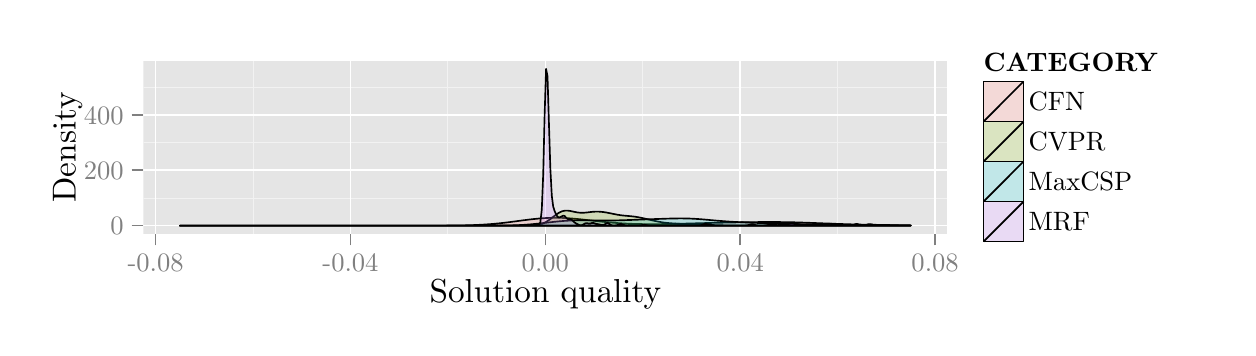
\begin{tikzpicture}[x=1pt,y=1pt]
\definecolor[named]{fillColor}{rgb}{1.00,1.00,1.00}
\path[use as bounding box,fill=fillColor,fill opacity=0.00] (0,0) rectangle (433.62,108.41);
\begin{scope}
\path[clip] (  0.00,  0.00) rectangle (433.62,108.40);
\definecolor[named]{drawColor}{rgb}{1.00,1.00,1.00}
\definecolor[named]{fillColor}{rgb}{1.00,1.00,1.00}

\path[draw=drawColor,line width= 0.6pt,line join=round,line cap=round,fill=fillColor] ( -0.00,  0.00) rectangle (433.62,108.40);
\end{scope}
\begin{scope}
\path[clip] ( 41.82, 34.03) rectangle (332.31, 96.36);
\definecolor[named]{fillColor}{rgb}{0.90,0.90,0.90}

\path[fill=fillColor] ( 41.82, 34.03) rectangle (332.31, 96.36);
\definecolor[named]{drawColor}{rgb}{0.95,0.95,0.95}

\path[draw=drawColor,line width= 0.3pt,line join=round] ( 41.82, 46.87) --
	(332.31, 46.87);

\path[draw=drawColor,line width= 0.3pt,line join=round] ( 41.82, 66.86) --
	(332.31, 66.86);

\path[draw=drawColor,line width= 0.3pt,line join=round] ( 41.82, 86.86) --
	(332.31, 86.86);

\path[draw=drawColor,line width= 0.3pt,line join=round] ( 81.43, 34.03) --
	( 81.43, 96.36);

\path[draw=drawColor,line width= 0.3pt,line join=round] (151.85, 34.03) --
	(151.85, 96.36);

\path[draw=drawColor,line width= 0.3pt,line join=round] (222.27, 34.03) --
	(222.27, 96.36);

\path[draw=drawColor,line width= 0.3pt,line join=round] (292.69, 34.03) --
	(292.69, 96.36);
\definecolor[named]{drawColor}{rgb}{1.00,1.00,1.00}

\path[draw=drawColor,line width= 0.6pt,line join=round] ( 41.82, 36.87) --
	(332.31, 36.87);

\path[draw=drawColor,line width= 0.6pt,line join=round] ( 41.82, 56.86) --
	(332.31, 56.86);

\path[draw=drawColor,line width= 0.6pt,line join=round] ( 41.82, 76.86) --
	(332.31, 76.86);

\path[draw=drawColor,line width= 0.6pt,line join=round] ( 46.22, 34.03) --
	( 46.22, 96.36);

\path[draw=drawColor,line width= 0.6pt,line join=round] (116.64, 34.03) --
	(116.64, 96.36);

\path[draw=drawColor,line width= 0.6pt,line join=round] (187.06, 34.03) --
	(187.06, 96.36);

\path[draw=drawColor,line width= 0.6pt,line join=round] (257.48, 34.03) --
	(257.48, 96.36);

\path[draw=drawColor,line width= 0.6pt,line join=round] (327.90, 34.03) --
	(327.90, 96.36);
\definecolor[named]{drawColor}{rgb}{0.00,0.00,0.00}
\definecolor[named]{fillColor}{rgb}{0.97,0.46,0.43}

\path[draw=drawColor,line width= 0.6pt,line join=round,line cap=round,fill=fillColor,fill opacity=0.20] ( 55.02, 36.87) --
	( 55.54, 36.87) --
	( 56.06, 36.87) --
	( 56.57, 36.87) --
	( 57.09, 36.87) --
	( 57.61, 36.87) --
	( 58.12, 36.87) --
	( 58.64, 36.87) --
	( 59.16, 36.87) --
	( 59.67, 36.87) --
	( 60.19, 36.87) --
	( 60.71, 36.87) --
	( 61.22, 36.87) --
	( 61.74, 36.87) --
	( 62.26, 36.87) --
	( 62.78, 36.87) --
	( 63.29, 36.87) --
	( 63.81, 36.87) --
	( 64.33, 36.87) --
	( 64.84, 36.87) --
	( 65.36, 36.87) --
	( 65.88, 36.87) --
	( 66.39, 36.87) --
	( 66.91, 36.87) --
	( 67.43, 36.87) --
	( 67.94, 36.87) --
	( 68.46, 36.87) --
	( 68.98, 36.87) --
	( 69.49, 36.87) --
	( 70.01, 36.87) --
	( 70.53, 36.87) --
	( 71.04, 36.87) --
	( 71.56, 36.87) --
	( 72.08, 36.87) --
	( 72.59, 36.87) --
	( 73.11, 36.87) --
	( 73.63, 36.87) --
	( 74.14, 36.87) --
	( 74.66, 36.87) --
	( 75.18, 36.87) --
	( 75.69, 36.87) --
	( 76.21, 36.87) --
	( 76.73, 36.87) --
	( 77.25, 36.87) --
	( 77.76, 36.87) --
	( 78.28, 36.87) --
	( 78.80, 36.87) --
	( 79.31, 36.87) --
	( 79.83, 36.87) --
	( 80.35, 36.87) --
	( 80.86, 36.87) --
	( 81.38, 36.87) --
	( 81.90, 36.87) --
	( 82.41, 36.87) --
	( 82.93, 36.87) --
	( 83.45, 36.87) --
	( 83.96, 36.87) --
	( 84.48, 36.87) --
	( 85.00, 36.87) --
	( 85.51, 36.87) --
	( 86.03, 36.87) --
	( 86.55, 36.87) --
	( 87.06, 36.87) --
	( 87.58, 36.87) --
	( 88.10, 36.87) --
	( 88.61, 36.87) --
	( 89.13, 36.87) --
	( 89.65, 36.87) --
	( 90.16, 36.87) --
	( 90.68, 36.87) --
	( 91.20, 36.87) --
	( 91.72, 36.87) --
	( 92.23, 36.87) --
	( 92.75, 36.87) --
	( 93.27, 36.87) --
	( 93.78, 36.87) --
	( 94.30, 36.87) --
	( 94.82, 36.87) --
	( 95.33, 36.87) --
	( 95.85, 36.87) --
	( 96.37, 36.87) --
	( 96.88, 36.87) --
	( 97.40, 36.87) --
	( 97.92, 36.87) --
	( 98.43, 36.87) --
	( 98.95, 36.87) --
	( 99.47, 36.87) --
	( 99.98, 36.87) --
	(100.50, 36.87) --
	(101.02, 36.87) --
	(101.53, 36.87) --
	(102.05, 36.87) --
	(102.57, 36.87) --
	(103.08, 36.87) --
	(103.60, 36.87) --
	(104.12, 36.87) --
	(104.63, 36.87) --
	(105.15, 36.87) --
	(105.67, 36.87) --
	(106.19, 36.87) --
	(106.70, 36.87) --
	(107.22, 36.87) --
	(107.74, 36.87) --
	(108.25, 36.87) --
	(108.77, 36.87) --
	(109.29, 36.87) --
	(109.80, 36.87) --
	(110.32, 36.87) --
	(110.84, 36.87) --
	(111.35, 36.87) --
	(111.87, 36.87) --
	(112.39, 36.87) --
	(112.90, 36.87) --
	(113.42, 36.87) --
	(113.94, 36.87) --
	(114.45, 36.87) --
	(114.97, 36.87) --
	(115.49, 36.87) --
	(116.00, 36.87) --
	(116.52, 36.87) --
	(117.04, 36.87) --
	(117.55, 36.87) --
	(118.07, 36.87) --
	(118.59, 36.87) --
	(119.10, 36.87) --
	(119.62, 36.87) --
	(120.14, 36.87) --
	(120.66, 36.87) --
	(121.17, 36.87) --
	(121.69, 36.87) --
	(122.21, 36.87) --
	(122.72, 36.87) --
	(123.24, 36.87) --
	(123.76, 36.87) --
	(124.27, 36.87) --
	(124.79, 36.87) --
	(125.31, 36.87) --
	(125.82, 36.87) --
	(126.34, 36.87) --
	(126.86, 36.87) --
	(127.37, 36.87) --
	(127.89, 36.87) --
	(128.41, 36.87) --
	(128.92, 36.87) --
	(129.44, 36.87) --
	(129.96, 36.87) --
	(130.47, 36.87) --
	(130.99, 36.87) --
	(131.51, 36.87) --
	(132.02, 36.87) --
	(132.54, 36.87) --
	(133.06, 36.87) --
	(133.57, 36.87) --
	(134.09, 36.87) --
	(134.61, 36.87) --
	(135.13, 36.87) --
	(135.64, 36.87) --
	(136.16, 36.87) --
	(136.68, 36.87) --
	(137.19, 36.87) --
	(137.71, 36.87) --
	(138.23, 36.87) --
	(138.74, 36.87) --
	(139.26, 36.87) --
	(139.78, 36.87) --
	(140.29, 36.87) --
	(140.81, 36.87) --
	(141.33, 36.87) --
	(141.84, 36.87) --
	(142.36, 36.87) --
	(142.88, 36.87) --
	(143.39, 36.87) --
	(143.91, 36.87) --
	(144.43, 36.87) --
	(144.94, 36.87) --
	(145.46, 36.87) --
	(145.98, 36.87) --
	(146.49, 36.88) --
	(147.01, 36.88) --
	(147.53, 36.88) --
	(148.04, 36.88) --
	(148.56, 36.88) --
	(149.08, 36.88) --
	(149.60, 36.88) --
	(150.11, 36.89) --
	(150.63, 36.89) --
	(151.15, 36.89) --
	(151.66, 36.90) --
	(152.18, 36.90) --
	(152.70, 36.90) --
	(153.21, 36.91) --
	(153.73, 36.91) --
	(154.25, 36.92) --
	(154.76, 36.93) --
	(155.28, 36.93) --
	(155.80, 36.94) --
	(156.31, 36.95) --
	(156.83, 36.96) --
	(157.35, 36.97) --
	(157.86, 36.98) --
	(158.38, 36.99) --
	(158.90, 37.01) --
	(159.41, 37.02) --
	(159.93, 37.04) --
	(160.45, 37.05) --
	(160.96, 37.07) --
	(161.48, 37.09) --
	(162.00, 37.11) --
	(162.51, 37.14) --
	(163.03, 37.16) --
	(163.55, 37.19) --
	(164.07, 37.21) --
	(164.58, 37.24) --
	(165.10, 37.28) --
	(165.62, 37.31) --
	(166.13, 37.35) --
	(166.65, 37.38) --
	(167.17, 37.42) --
	(167.68, 37.46) --
	(168.20, 37.51) --
	(168.72, 37.55) --
	(169.23, 37.60) --
	(169.75, 37.65) --
	(170.27, 37.70) --
	(170.78, 37.76) --
	(171.30, 37.81) --
	(171.82, 37.87) --
	(172.33, 37.93) --
	(172.85, 37.99) --
	(173.37, 38.05) --
	(173.88, 38.12) --
	(174.40, 38.18) --
	(174.92, 38.25) --
	(175.43, 38.32) --
	(175.95, 38.38) --
	(176.47, 38.45) --
	(176.98, 38.52) --
	(177.50, 38.59) --
	(178.02, 38.66) --
	(178.54, 38.73) --
	(179.05, 38.80) --
	(179.57, 38.86) --
	(180.09, 38.93) --
	(180.60, 38.99) --
	(181.12, 39.06) --
	(181.64, 39.12) --
	(182.15, 39.18) --
	(182.67, 39.24) --
	(183.19, 39.29) --
	(183.70, 39.34) --
	(184.22, 39.39) --
	(184.74, 39.44) --
	(185.25, 39.48) --
	(185.77, 39.52) --
	(186.29, 39.56) --
	(186.80, 39.59) --
	(187.32, 39.62) --
	(187.84, 39.65) --
	(188.35, 39.67) --
	(188.87, 39.69) --
	(189.39, 39.70) --
	(189.90, 39.71) --
	(190.42, 39.71) --
	(190.94, 39.71) --
	(191.46, 39.71) --
	(191.97, 39.70) --
	(192.49, 39.69) --
	(193.01, 39.67) --
	(193.52, 39.65) --
	(194.04, 39.63) --
	(194.56, 39.60) --
	(195.07, 39.57) --
	(195.59, 39.53) --
	(196.11, 39.50) --
	(196.62, 39.46) --
	(197.14, 39.41) --
	(197.66, 39.37) --
	(198.17, 39.32) --
	(198.69, 39.27) --
	(199.21, 39.22) --
	(199.72, 39.17) --
	(200.24, 39.11) --
	(200.76, 39.06) --
	(201.27, 39.00) --
	(201.79, 38.94) --
	(202.31, 38.88) --
	(202.82, 38.83) --
	(203.34, 38.77) --
	(203.86, 38.71) --
	(204.37, 38.65) --
	(204.89, 38.59) --
	(205.41, 38.53) --
	(205.93, 38.48) --
	(206.44, 38.42) --
	(206.96, 38.36) --
	(207.48, 38.31) --
	(207.99, 38.26) --
	(208.51, 38.20) --
	(209.03, 38.15) --
	(209.54, 38.10) --
	(210.06, 38.06) --
	(210.58, 38.01) --
	(211.09, 37.97) --
	(211.61, 37.92) --
	(212.13, 37.88) --
	(212.64, 37.84) --
	(213.16, 37.81) --
	(213.68, 37.77) --
	(214.19, 37.74) --
	(214.71, 37.71) --
	(215.23, 37.68) --
	(215.74, 37.65) --
	(216.26, 37.62) --
	(216.78, 37.60) --
	(217.29, 37.57) --
	(217.81, 37.55) --
	(218.33, 37.53) --
	(218.84, 37.52) --
	(219.36, 37.50) --
	(219.88, 37.48) --
	(220.40, 37.47) --
	(220.91, 37.46) --
	(221.43, 37.45) --
	(221.95, 37.44) --
	(222.46, 37.43) --
	(222.98, 37.43) --
	(223.50, 37.42) --
	(224.01, 37.42) --
	(224.53, 37.42) --
	(225.05, 37.42) --
	(225.56, 37.42) --
	(226.08, 37.42) --
	(226.60, 37.42) --
	(227.11, 37.42) --
	(227.63, 37.42) --
	(228.15, 37.43) --
	(228.66, 37.43) --
	(229.18, 37.44) --
	(229.70, 37.45) --
	(230.21, 37.46) --
	(230.73, 37.46) --
	(231.25, 37.47) --
	(231.76, 37.48) --
	(232.28, 37.49) --
	(232.80, 37.50) --
	(233.31, 37.51) --
	(233.83, 37.52) --
	(234.35, 37.54) --
	(234.87, 37.55) --
	(235.38, 37.56) --
	(235.90, 37.57) --
	(236.42, 37.59) --
	(236.93, 37.60) --
	(237.45, 37.61) --
	(237.97, 37.62) --
	(238.48, 37.64) --
	(239.00, 37.65) --
	(239.52, 37.66) --
	(240.03, 37.68) --
	(240.55, 37.69) --
	(241.07, 37.70) --
	(241.58, 37.72) --
	(242.10, 37.73) --
	(242.62, 37.74) --
	(243.13, 37.76) --
	(243.65, 37.77) --
	(244.17, 37.78) --
	(244.68, 37.80) --
	(245.20, 37.81) --
	(245.72, 37.82) --
	(246.23, 37.83) --
	(246.75, 37.85) --
	(247.27, 37.86) --
	(247.78, 37.87) --
	(248.30, 37.88) --
	(248.82, 37.89) --
	(249.34, 37.91) --
	(249.85, 37.92) --
	(250.37, 37.93) --
	(250.89, 37.94) --
	(251.40, 37.95) --
	(251.92, 37.96) --
	(252.44, 37.97) --
	(252.95, 37.98) --
	(253.47, 37.99) --
	(253.99, 38.00) --
	(254.50, 38.01) --
	(255.02, 38.02) --
	(255.54, 38.03) --
	(256.05, 38.04) --
	(256.57, 38.05) --
	(257.09, 38.06) --
	(257.60, 38.07) --
	(258.12, 38.08) --
	(258.64, 38.09) --
	(259.15, 38.10) --
	(259.67, 38.11) --
	(260.19, 38.12) --
	(260.70, 38.12) --
	(261.22, 38.13) --
	(261.74, 38.14) --
	(262.25, 38.15) --
	(262.77, 38.15) --
	(263.29, 38.16) --
	(263.81, 38.16) --
	(264.32, 38.17) --
	(264.84, 38.17) --
	(265.36, 38.18) --
	(265.87, 38.18) --
	(266.39, 38.18) --
	(266.91, 38.18) --
	(267.42, 38.18) --
	(267.94, 38.19) --
	(268.46, 38.19) --
	(268.97, 38.18) --
	(269.49, 38.18) --
	(270.01, 38.18) --
	(270.52, 38.18) --
	(271.04, 38.17) --
	(271.56, 38.17) --
	(272.07, 38.16) --
	(272.59, 38.16) --
	(273.11, 38.15) --
	(273.62, 38.14) --
	(274.14, 38.13) --
	(274.66, 38.12) --
	(275.17, 38.11) --
	(275.69, 38.10) --
	(276.21, 38.09) --
	(276.72, 38.08) --
	(277.24, 38.07) --
	(277.76, 38.05) --
	(278.28, 38.04) --
	(278.79, 38.02) --
	(279.31, 38.01) --
	(279.83, 37.99) --
	(280.34, 37.97) --
	(280.86, 37.96) --
	(281.38, 37.94) --
	(281.89, 37.92) --
	(282.41, 37.90) --
	(282.93, 37.88) --
	(283.44, 37.86) --
	(283.96, 37.84) --
	(284.48, 37.82) --
	(284.99, 37.80) --
	(285.51, 37.78) --
	(286.03, 37.76) --
	(286.54, 37.74) --
	(287.06, 37.72) --
	(287.58, 37.70) --
	(288.09, 37.68) --
	(288.61, 37.66) --
	(289.13, 37.64) --
	(289.64, 37.62) --
	(290.16, 37.60) --
	(290.68, 37.58) --
	(291.19, 37.56) --
	(291.71, 37.54) --
	(292.23, 37.52) --
	(292.75, 37.50) --
	(293.26, 37.48) --
	(293.78, 37.47) --
	(294.30, 37.45) --
	(294.81, 37.43) --
	(295.33, 37.41) --
	(295.85, 37.40) --
	(296.36, 37.38) --
	(296.88, 37.37) --
	(297.40, 37.35) --
	(297.91, 37.34) --
	(298.43, 37.32) --
	(298.95, 37.31) --
	(299.46, 37.30) --
	(299.98, 37.28) --
	(300.50, 37.27) --
	(301.01, 37.26) --
	(301.53, 37.25) --
	(302.05, 37.24) --
	(302.56, 37.22) --
	(303.08, 37.21) --
	(303.60, 37.20) --
	(304.11, 37.19) --
	(304.63, 37.18) --
	(305.15, 37.17) --
	(305.66, 37.16) --
	(306.18, 37.15) --
	(306.70, 37.15) --
	(307.22, 37.14) --
	(307.73, 37.13) --
	(308.25, 37.12) --
	(308.77, 37.11) --
	(309.28, 37.11) --
	(309.80, 37.10) --
	(310.32, 37.09) --
	(310.83, 37.08) --
	(311.35, 37.08) --
	(311.87, 37.07) --
	(312.38, 37.06) --
	(312.90, 37.06) --
	(313.42, 37.05) --
	(313.93, 37.04) --
	(314.45, 37.04) --
	(314.97, 37.03) --
	(315.48, 37.02) --
	(316.00, 37.02) --
	(316.52, 37.01) --
	(317.03, 37.01) --
	(317.55, 37.00) --
	(318.07, 36.99) --
	(318.58, 36.99) --
	(319.10, 36.98) --
	(319.10, 36.87) --
	(318.58, 36.87) --
	(318.07, 36.87) --
	(317.55, 36.87) --
	(317.03, 36.87) --
	(316.52, 36.87) --
	(316.00, 36.87) --
	(315.48, 36.87) --
	(314.97, 36.87) --
	(314.45, 36.87) --
	(313.93, 36.87) --
	(313.42, 36.87) --
	(312.90, 36.87) --
	(312.38, 36.87) --
	(311.87, 36.87) --
	(311.35, 36.87) --
	(310.83, 36.87) --
	(310.32, 36.87) --
	(309.80, 36.87) --
	(309.28, 36.87) --
	(308.77, 36.87) --
	(308.25, 36.87) --
	(307.73, 36.87) --
	(307.22, 36.87) --
	(306.70, 36.87) --
	(306.18, 36.87) --
	(305.66, 36.87) --
	(305.15, 36.87) --
	(304.63, 36.87) --
	(304.11, 36.87) --
	(303.60, 36.87) --
	(303.08, 36.87) --
	(302.56, 36.87) --
	(302.05, 36.87) --
	(301.53, 36.87) --
	(301.01, 36.87) --
	(300.50, 36.87) --
	(299.98, 36.87) --
	(299.46, 36.87) --
	(298.95, 36.87) --
	(298.43, 36.87) --
	(297.91, 36.87) --
	(297.40, 36.87) --
	(296.88, 36.87) --
	(296.36, 36.87) --
	(295.85, 36.87) --
	(295.33, 36.87) --
	(294.81, 36.87) --
	(294.30, 36.87) --
	(293.78, 36.87) --
	(293.26, 36.87) --
	(292.75, 36.87) --
	(292.23, 36.87) --
	(291.71, 36.87) --
	(291.19, 36.87) --
	(290.68, 36.87) --
	(290.16, 36.87) --
	(289.64, 36.87) --
	(289.13, 36.87) --
	(288.61, 36.87) --
	(288.09, 36.87) --
	(287.58, 36.87) --
	(287.06, 36.87) --
	(286.54, 36.87) --
	(286.03, 36.87) --
	(285.51, 36.87) --
	(284.99, 36.87) --
	(284.48, 36.87) --
	(283.96, 36.87) --
	(283.44, 36.87) --
	(282.93, 36.87) --
	(282.41, 36.87) --
	(281.89, 36.87) --
	(281.38, 36.87) --
	(280.86, 36.87) --
	(280.34, 36.87) --
	(279.83, 36.87) --
	(279.31, 36.87) --
	(278.79, 36.87) --
	(278.28, 36.87) --
	(277.76, 36.87) --
	(277.24, 36.87) --
	(276.72, 36.87) --
	(276.21, 36.87) --
	(275.69, 36.87) --
	(275.17, 36.87) --
	(274.66, 36.87) --
	(274.14, 36.87) --
	(273.62, 36.87) --
	(273.11, 36.87) --
	(272.59, 36.87) --
	(272.07, 36.87) --
	(271.56, 36.87) --
	(271.04, 36.87) --
	(270.52, 36.87) --
	(270.01, 36.87) --
	(269.49, 36.87) --
	(268.97, 36.87) --
	(268.46, 36.87) --
	(267.94, 36.87) --
	(267.42, 36.87) --
	(266.91, 36.87) --
	(266.39, 36.87) --
	(265.87, 36.87) --
	(265.36, 36.87) --
	(264.84, 36.87) --
	(264.32, 36.87) --
	(263.81, 36.87) --
	(263.29, 36.87) --
	(262.77, 36.87) --
	(262.25, 36.87) --
	(261.74, 36.87) --
	(261.22, 36.87) --
	(260.70, 36.87) --
	(260.19, 36.87) --
	(259.67, 36.87) --
	(259.15, 36.87) --
	(258.64, 36.87) --
	(258.12, 36.87) --
	(257.60, 36.87) --
	(257.09, 36.87) --
	(256.57, 36.87) --
	(256.05, 36.87) --
	(255.54, 36.87) --
	(255.02, 36.87) --
	(254.50, 36.87) --
	(253.99, 36.87) --
	(253.47, 36.87) --
	(252.95, 36.87) --
	(252.44, 36.87) --
	(251.92, 36.87) --
	(251.40, 36.87) --
	(250.89, 36.87) --
	(250.37, 36.87) --
	(249.85, 36.87) --
	(249.34, 36.87) --
	(248.82, 36.87) --
	(248.30, 36.87) --
	(247.78, 36.87) --
	(247.27, 36.87) --
	(246.75, 36.87) --
	(246.23, 36.87) --
	(245.72, 36.87) --
	(245.20, 36.87) --
	(244.68, 36.87) --
	(244.17, 36.87) --
	(243.65, 36.87) --
	(243.13, 36.87) --
	(242.62, 36.87) --
	(242.10, 36.87) --
	(241.58, 36.87) --
	(241.07, 36.87) --
	(240.55, 36.87) --
	(240.03, 36.87) --
	(239.52, 36.87) --
	(239.00, 36.87) --
	(238.48, 36.87) --
	(237.97, 36.87) --
	(237.45, 36.87) --
	(236.93, 36.87) --
	(236.42, 36.87) --
	(235.90, 36.87) --
	(235.38, 36.87) --
	(234.87, 36.87) --
	(234.35, 36.87) --
	(233.83, 36.87) --
	(233.31, 36.87) --
	(232.80, 36.87) --
	(232.28, 36.87) --
	(231.76, 36.87) --
	(231.25, 36.87) --
	(230.73, 36.87) --
	(230.21, 36.87) --
	(229.70, 36.87) --
	(229.18, 36.87) --
	(228.66, 36.87) --
	(228.15, 36.87) --
	(227.63, 36.87) --
	(227.11, 36.87) --
	(226.60, 36.87) --
	(226.08, 36.87) --
	(225.56, 36.87) --
	(225.05, 36.87) --
	(224.53, 36.87) --
	(224.01, 36.87) --
	(223.50, 36.87) --
	(222.98, 36.87) --
	(222.46, 36.87) --
	(221.95, 36.87) --
	(221.43, 36.87) --
	(220.91, 36.87) --
	(220.40, 36.87) --
	(219.88, 36.87) --
	(219.36, 36.87) --
	(218.84, 36.87) --
	(218.33, 36.87) --
	(217.81, 36.87) --
	(217.29, 36.87) --
	(216.78, 36.87) --
	(216.26, 36.87) --
	(215.74, 36.87) --
	(215.23, 36.87) --
	(214.71, 36.87) --
	(214.19, 36.87) --
	(213.68, 36.87) --
	(213.16, 36.87) --
	(212.64, 36.87) --
	(212.13, 36.87) --
	(211.61, 36.87) --
	(211.09, 36.87) --
	(210.58, 36.87) --
	(210.06, 36.87) --
	(209.54, 36.87) --
	(209.03, 36.87) --
	(208.51, 36.87) --
	(207.99, 36.87) --
	(207.48, 36.87) --
	(206.96, 36.87) --
	(206.44, 36.87) --
	(205.93, 36.87) --
	(205.41, 36.87) --
	(204.89, 36.87) --
	(204.37, 36.87) --
	(203.86, 36.87) --
	(203.34, 36.87) --
	(202.82, 36.87) --
	(202.31, 36.87) --
	(201.79, 36.87) --
	(201.27, 36.87) --
	(200.76, 36.87) --
	(200.24, 36.87) --
	(199.72, 36.87) --
	(199.21, 36.87) --
	(198.69, 36.87) --
	(198.17, 36.87) --
	(197.66, 36.87) --
	(197.14, 36.87) --
	(196.62, 36.87) --
	(196.11, 36.87) --
	(195.59, 36.87) --
	(195.07, 36.87) --
	(194.56, 36.87) --
	(194.04, 36.87) --
	(193.52, 36.87) --
	(193.01, 36.87) --
	(192.49, 36.87) --
	(191.97, 36.87) --
	(191.46, 36.87) --
	(190.94, 36.87) --
	(190.42, 36.87) --
	(189.90, 36.87) --
	(189.39, 36.87) --
	(188.87, 36.87) --
	(188.35, 36.87) --
	(187.84, 36.87) --
	(187.32, 36.87) --
	(186.80, 36.87) --
	(186.29, 36.87) --
	(185.77, 36.87) --
	(185.25, 36.87) --
	(184.74, 36.87) --
	(184.22, 36.87) --
	(183.70, 36.87) --
	(183.19, 36.87) --
	(182.67, 36.87) --
	(182.15, 36.87) --
	(181.64, 36.87) --
	(181.12, 36.87) --
	(180.60, 36.87) --
	(180.09, 36.87) --
	(179.57, 36.87) --
	(179.05, 36.87) --
	(178.54, 36.87) --
	(178.02, 36.87) --
	(177.50, 36.87) --
	(176.98, 36.87) --
	(176.47, 36.87) --
	(175.95, 36.87) --
	(175.43, 36.87) --
	(174.92, 36.87) --
	(174.40, 36.87) --
	(173.88, 36.87) --
	(173.37, 36.87) --
	(172.85, 36.87) --
	(172.33, 36.87) --
	(171.82, 36.87) --
	(171.30, 36.87) --
	(170.78, 36.87) --
	(170.27, 36.87) --
	(169.75, 36.87) --
	(169.23, 36.87) --
	(168.72, 36.87) --
	(168.20, 36.87) --
	(167.68, 36.87) --
	(167.17, 36.87) --
	(166.65, 36.87) --
	(166.13, 36.87) --
	(165.62, 36.87) --
	(165.10, 36.87) --
	(164.58, 36.87) --
	(164.07, 36.87) --
	(163.55, 36.87) --
	(163.03, 36.87) --
	(162.51, 36.87) --
	(162.00, 36.87) --
	(161.48, 36.87) --
	(160.96, 36.87) --
	(160.45, 36.87) --
	(159.93, 36.87) --
	(159.41, 36.87) --
	(158.90, 36.87) --
	(158.38, 36.87) --
	(157.86, 36.87) --
	(157.35, 36.87) --
	(156.83, 36.87) --
	(156.31, 36.87) --
	(155.80, 36.87) --
	(155.28, 36.87) --
	(154.76, 36.87) --
	(154.25, 36.87) --
	(153.73, 36.87) --
	(153.21, 36.87) --
	(152.70, 36.87) --
	(152.18, 36.87) --
	(151.66, 36.87) --
	(151.15, 36.87) --
	(150.63, 36.87) --
	(150.11, 36.87) --
	(149.60, 36.87) --
	(149.08, 36.87) --
	(148.56, 36.87) --
	(148.04, 36.87) --
	(147.53, 36.87) --
	(147.01, 36.87) --
	(146.49, 36.87) --
	(145.98, 36.87) --
	(145.46, 36.87) --
	(144.94, 36.87) --
	(144.43, 36.87) --
	(143.91, 36.87) --
	(143.39, 36.87) --
	(142.88, 36.87) --
	(142.36, 36.87) --
	(141.84, 36.87) --
	(141.33, 36.87) --
	(140.81, 36.87) --
	(140.29, 36.87) --
	(139.78, 36.87) --
	(139.26, 36.87) --
	(138.74, 36.87) --
	(138.23, 36.87) --
	(137.71, 36.87) --
	(137.19, 36.87) --
	(136.68, 36.87) --
	(136.16, 36.87) --
	(135.64, 36.87) --
	(135.13, 36.87) --
	(134.61, 36.87) --
	(134.09, 36.87) --
	(133.57, 36.87) --
	(133.06, 36.87) --
	(132.54, 36.87) --
	(132.02, 36.87) --
	(131.51, 36.87) --
	(130.99, 36.87) --
	(130.47, 36.87) --
	(129.96, 36.87) --
	(129.44, 36.87) --
	(128.92, 36.87) --
	(128.41, 36.87) --
	(127.89, 36.87) --
	(127.37, 36.87) --
	(126.86, 36.87) --
	(126.34, 36.87) --
	(125.82, 36.87) --
	(125.31, 36.87) --
	(124.79, 36.87) --
	(124.27, 36.87) --
	(123.76, 36.87) --
	(123.24, 36.87) --
	(122.72, 36.87) --
	(122.21, 36.87) --
	(121.69, 36.87) --
	(121.17, 36.87) --
	(120.66, 36.87) --
	(120.14, 36.87) --
	(119.62, 36.87) --
	(119.10, 36.87) --
	(118.59, 36.87) --
	(118.07, 36.87) --
	(117.55, 36.87) --
	(117.04, 36.87) --
	(116.52, 36.87) --
	(116.00, 36.87) --
	(115.49, 36.87) --
	(114.97, 36.87) --
	(114.45, 36.87) --
	(113.94, 36.87) --
	(113.42, 36.87) --
	(112.90, 36.87) --
	(112.39, 36.87) --
	(111.87, 36.87) --
	(111.35, 36.87) --
	(110.84, 36.87) --
	(110.32, 36.87) --
	(109.80, 36.87) --
	(109.29, 36.87) --
	(108.77, 36.87) --
	(108.25, 36.87) --
	(107.74, 36.87) --
	(107.22, 36.87) --
	(106.70, 36.87) --
	(106.19, 36.87) --
	(105.67, 36.87) --
	(105.15, 36.87) --
	(104.63, 36.87) --
	(104.12, 36.87) --
	(103.60, 36.87) --
	(103.08, 36.87) --
	(102.57, 36.87) --
	(102.05, 36.87) --
	(101.53, 36.87) --
	(101.02, 36.87) --
	(100.50, 36.87) --
	( 99.98, 36.87) --
	( 99.47, 36.87) --
	( 98.95, 36.87) --
	( 98.43, 36.87) --
	( 97.92, 36.87) --
	( 97.40, 36.87) --
	( 96.88, 36.87) --
	( 96.37, 36.87) --
	( 95.85, 36.87) --
	( 95.33, 36.87) --
	( 94.82, 36.87) --
	( 94.30, 36.87) --
	( 93.78, 36.87) --
	( 93.27, 36.87) --
	( 92.75, 36.87) --
	( 92.23, 36.87) --
	( 91.72, 36.87) --
	( 91.20, 36.87) --
	( 90.68, 36.87) --
	( 90.16, 36.87) --
	( 89.65, 36.87) --
	( 89.13, 36.87) --
	( 88.61, 36.87) --
	( 88.10, 36.87) --
	( 87.58, 36.87) --
	( 87.06, 36.87) --
	( 86.55, 36.87) --
	( 86.03, 36.87) --
	( 85.51, 36.87) --
	( 85.00, 36.87) --
	( 84.48, 36.87) --
	( 83.96, 36.87) --
	( 83.45, 36.87) --
	( 82.93, 36.87) --
	( 82.41, 36.87) --
	( 81.90, 36.87) --
	( 81.38, 36.87) --
	( 80.86, 36.87) --
	( 80.35, 36.87) --
	( 79.83, 36.87) --
	( 79.31, 36.87) --
	( 78.80, 36.87) --
	( 78.28, 36.87) --
	( 77.76, 36.87) --
	( 77.25, 36.87) --
	( 76.73, 36.87) --
	( 76.21, 36.87) --
	( 75.69, 36.87) --
	( 75.18, 36.87) --
	( 74.66, 36.87) --
	( 74.14, 36.87) --
	( 73.63, 36.87) --
	( 73.11, 36.87) --
	( 72.59, 36.87) --
	( 72.08, 36.87) --
	( 71.56, 36.87) --
	( 71.04, 36.87) --
	( 70.53, 36.87) --
	( 70.01, 36.87) --
	( 69.49, 36.87) --
	( 68.98, 36.87) --
	( 68.46, 36.87) --
	( 67.94, 36.87) --
	( 67.43, 36.87) --
	( 66.91, 36.87) --
	( 66.39, 36.87) --
	( 65.88, 36.87) --
	( 65.36, 36.87) --
	( 64.84, 36.87) --
	( 64.33, 36.87) --
	( 63.81, 36.87) --
	( 63.29, 36.87) --
	( 62.78, 36.87) --
	( 62.26, 36.87) --
	( 61.74, 36.87) --
	( 61.22, 36.87) --
	( 60.71, 36.87) --
	( 60.19, 36.87) --
	( 59.67, 36.87) --
	( 59.16, 36.87) --
	( 58.64, 36.87) --
	( 58.12, 36.87) --
	( 57.61, 36.87) --
	( 57.09, 36.87) --
	( 56.57, 36.87) --
	( 56.06, 36.87) --
	( 55.54, 36.87) --
	( 55.02, 36.87) --
	cycle;
\definecolor[named]{fillColor}{rgb}{0.49,0.68,0.00}

\path[draw=drawColor,line width= 0.6pt,line join=round,line cap=round,fill=fillColor,fill opacity=0.20] ( 55.02, 36.87) --
	( 55.54, 36.87) --
	( 56.06, 36.87) --
	( 56.57, 36.87) --
	( 57.09, 36.87) --
	( 57.61, 36.87) --
	( 58.12, 36.87) --
	( 58.64, 36.87) --
	( 59.16, 36.87) --
	( 59.67, 36.87) --
	( 60.19, 36.87) --
	( 60.71, 36.87) --
	( 61.22, 36.87) --
	( 61.74, 36.87) --
	( 62.26, 36.87) --
	( 62.78, 36.87) --
	( 63.29, 36.87) --
	( 63.81, 36.87) --
	( 64.33, 36.87) --
	( 64.84, 36.87) --
	( 65.36, 36.87) --
	( 65.88, 36.87) --
	( 66.39, 36.87) --
	( 66.91, 36.87) --
	( 67.43, 36.87) --
	( 67.94, 36.87) --
	( 68.46, 36.87) --
	( 68.98, 36.87) --
	( 69.49, 36.87) --
	( 70.01, 36.87) --
	( 70.53, 36.87) --
	( 71.04, 36.87) --
	( 71.56, 36.87) --
	( 72.08, 36.87) --
	( 72.59, 36.87) --
	( 73.11, 36.87) --
	( 73.63, 36.87) --
	( 74.14, 36.87) --
	( 74.66, 36.87) --
	( 75.18, 36.87) --
	( 75.69, 36.87) --
	( 76.21, 36.87) --
	( 76.73, 36.87) --
	( 77.25, 36.87) --
	( 77.76, 36.87) --
	( 78.28, 36.87) --
	( 78.80, 36.87) --
	( 79.31, 36.87) --
	( 79.83, 36.87) --
	( 80.35, 36.87) --
	( 80.86, 36.87) --
	( 81.38, 36.87) --
	( 81.90, 36.87) --
	( 82.41, 36.87) --
	( 82.93, 36.87) --
	( 83.45, 36.87) --
	( 83.96, 36.87) --
	( 84.48, 36.87) --
	( 85.00, 36.87) --
	( 85.51, 36.87) --
	( 86.03, 36.87) --
	( 86.55, 36.87) --
	( 87.06, 36.87) --
	( 87.58, 36.87) --
	( 88.10, 36.87) --
	( 88.61, 36.87) --
	( 89.13, 36.87) --
	( 89.65, 36.87) --
	( 90.16, 36.87) --
	( 90.68, 36.87) --
	( 91.20, 36.87) --
	( 91.72, 36.87) --
	( 92.23, 36.87) --
	( 92.75, 36.87) --
	( 93.27, 36.87) --
	( 93.78, 36.87) --
	( 94.30, 36.87) --
	( 94.82, 36.87) --
	( 95.33, 36.87) --
	( 95.85, 36.87) --
	( 96.37, 36.87) --
	( 96.88, 36.87) --
	( 97.40, 36.87) --
	( 97.92, 36.87) --
	( 98.43, 36.87) --
	( 98.95, 36.87) --
	( 99.47, 36.87) --
	( 99.98, 36.87) --
	(100.50, 36.87) --
	(101.02, 36.87) --
	(101.53, 36.87) --
	(102.05, 36.87) --
	(102.57, 36.87) --
	(103.08, 36.87) --
	(103.60, 36.87) --
	(104.12, 36.87) --
	(104.63, 36.87) --
	(105.15, 36.87) --
	(105.67, 36.87) --
	(106.19, 36.87) --
	(106.70, 36.87) --
	(107.22, 36.87) --
	(107.74, 36.87) --
	(108.25, 36.87) --
	(108.77, 36.87) --
	(109.29, 36.87) --
	(109.80, 36.87) --
	(110.32, 36.87) --
	(110.84, 36.87) --
	(111.35, 36.87) --
	(111.87, 36.87) --
	(112.39, 36.87) --
	(112.90, 36.87) --
	(113.42, 36.87) --
	(113.94, 36.87) --
	(114.45, 36.87) --
	(114.97, 36.87) --
	(115.49, 36.87) --
	(116.00, 36.87) --
	(116.52, 36.87) --
	(117.04, 36.87) --
	(117.55, 36.87) --
	(118.07, 36.87) --
	(118.59, 36.87) --
	(119.10, 36.87) --
	(119.62, 36.87) --
	(120.14, 36.87) --
	(120.66, 36.87) --
	(121.17, 36.87) --
	(121.69, 36.87) --
	(122.21, 36.87) --
	(122.72, 36.87) --
	(123.24, 36.87) --
	(123.76, 36.87) --
	(124.27, 36.87) --
	(124.79, 36.87) --
	(125.31, 36.87) --
	(125.82, 36.87) --
	(126.34, 36.87) --
	(126.86, 36.87) --
	(127.37, 36.87) --
	(127.89, 36.87) --
	(128.41, 36.87) --
	(128.92, 36.87) --
	(129.44, 36.87) --
	(129.96, 36.87) --
	(130.47, 36.87) --
	(130.99, 36.87) --
	(131.51, 36.87) --
	(132.02, 36.87) --
	(132.54, 36.87) --
	(133.06, 36.87) --
	(133.57, 36.87) --
	(134.09, 36.87) --
	(134.61, 36.87) --
	(135.13, 36.87) --
	(135.64, 36.87) --
	(136.16, 36.87) --
	(136.68, 36.87) --
	(137.19, 36.87) --
	(137.71, 36.87) --
	(138.23, 36.87) --
	(138.74, 36.87) --
	(139.26, 36.87) --
	(139.78, 36.87) --
	(140.29, 36.87) --
	(140.81, 36.87) --
	(141.33, 36.87) --
	(141.84, 36.87) --
	(142.36, 36.87) --
	(142.88, 36.87) --
	(143.39, 36.87) --
	(143.91, 36.87) --
	(144.43, 36.87) --
	(144.94, 36.87) --
	(145.46, 36.87) --
	(145.98, 36.87) --
	(146.49, 36.87) --
	(147.01, 36.87) --
	(147.53, 36.87) --
	(148.04, 36.87) --
	(148.56, 36.87) --
	(149.08, 36.87) --
	(149.60, 36.87) --
	(150.11, 36.87) --
	(150.63, 36.87) --
	(151.15, 36.87) --
	(151.66, 36.87) --
	(152.18, 36.87) --
	(152.70, 36.87) --
	(153.21, 36.87) --
	(153.73, 36.87) --
	(154.25, 36.87) --
	(154.76, 36.87) --
	(155.28, 36.87) --
	(155.80, 36.87) --
	(156.31, 36.87) --
	(156.83, 36.87) --
	(157.35, 36.87) --
	(157.86, 36.87) --
	(158.38, 36.87) --
	(158.90, 36.87) --
	(159.41, 36.87) --
	(159.93, 36.87) --
	(160.45, 36.87) --
	(160.96, 36.87) --
	(161.48, 36.87) --
	(162.00, 36.87) --
	(162.51, 36.87) --
	(163.03, 36.87) --
	(163.55, 36.87) --
	(164.07, 36.87) --
	(164.58, 36.87) --
	(165.10, 36.87) --
	(165.62, 36.87) --
	(166.13, 36.87) --
	(166.65, 36.87) --
	(167.17, 36.87) --
	(167.68, 36.87) --
	(168.20, 36.87) --
	(168.72, 36.87) --
	(169.23, 36.87) --
	(169.75, 36.87) --
	(170.27, 36.87) --
	(170.78, 36.87) --
	(171.30, 36.87) --
	(171.82, 36.87) --
	(172.33, 36.87) --
	(172.85, 36.87) --
	(173.37, 36.87) --
	(173.88, 36.87) --
	(174.40, 36.87) --
	(174.92, 36.87) --
	(175.43, 36.87) --
	(175.95, 36.87) --
	(176.47, 36.87) --
	(176.98, 36.87) --
	(177.50, 36.87) --
	(178.02, 36.87) --
	(178.54, 36.87) --
	(179.05, 36.87) --
	(179.57, 36.88) --
	(180.09, 36.88) --
	(180.60, 36.89) --
	(181.12, 36.90) --
	(181.64, 36.91) --
	(182.15, 36.94) --
	(182.67, 36.97) --
	(183.19, 37.01) --
	(183.70, 37.07) --
	(184.22, 37.15) --
	(184.74, 37.25) --
	(185.25, 37.37) --
	(185.77, 37.53) --
	(186.29, 37.72) --
	(186.80, 37.95) --
	(187.32, 38.22) --
	(187.84, 38.53) --
	(188.35, 38.87) --
	(188.87, 39.24) --
	(189.39, 39.64) --
	(189.90, 40.04) --
	(190.42, 40.44) --
	(190.94, 40.83) --
	(191.46, 41.19) --
	(191.97, 41.52) --
	(192.49, 41.80) --
	(193.01, 42.02) --
	(193.52, 42.17) --
	(194.04, 42.27) --
	(194.56, 42.31) --
	(195.07, 42.30) --
	(195.59, 42.25) --
	(196.11, 42.16) --
	(196.62, 42.06) --
	(197.14, 41.95) --
	(197.66, 41.83) --
	(198.17, 41.73) --
	(198.69, 41.64) --
	(199.21, 41.58) --
	(199.72, 41.54) --
	(200.24, 41.52) --
	(200.76, 41.53) --
	(201.27, 41.56) --
	(201.79, 41.61) --
	(202.31, 41.66) --
	(202.82, 41.72) --
	(203.34, 41.79) --
	(203.86, 41.84) --
	(204.37, 41.89) --
	(204.89, 41.92) --
	(205.41, 41.94) --
	(205.93, 41.94) --
	(206.44, 41.93) --
	(206.96, 41.89) --
	(207.48, 41.85) --
	(207.99, 41.79) --
	(208.51, 41.71) --
	(209.03, 41.63) --
	(209.54, 41.54) --
	(210.06, 41.44) --
	(210.58, 41.33) --
	(211.09, 41.22) --
	(211.61, 41.12) --
	(212.13, 41.01) --
	(212.64, 40.91) --
	(213.16, 40.82) --
	(213.68, 40.74) --
	(214.19, 40.66) --
	(214.71, 40.59) --
	(215.23, 40.53) --
	(215.74, 40.48) --
	(216.26, 40.43) --
	(216.78, 40.39) --
	(217.29, 40.34) --
	(217.81, 40.30) --
	(218.33, 40.24) --
	(218.84, 40.18) --
	(219.36, 40.12) --
	(219.88, 40.04) --
	(220.40, 39.95) --
	(220.91, 39.86) --
	(221.43, 39.76) --
	(221.95, 39.65) --
	(222.46, 39.54) --
	(222.98, 39.42) --
	(223.50, 39.30) --
	(224.01, 39.18) --
	(224.53, 39.06) --
	(225.05, 38.93) --
	(225.56, 38.81) --
	(226.08, 38.70) --
	(226.60, 38.58) --
	(227.11, 38.47) --
	(227.63, 38.37) --
	(228.15, 38.27) --
	(228.66, 38.18) --
	(229.18, 38.09) --
	(229.70, 38.02) --
	(230.21, 37.95) --
	(230.73, 37.89) --
	(231.25, 37.84) --
	(231.76, 37.79) --
	(232.28, 37.75) --
	(232.80, 37.71) --
	(233.31, 37.68) --
	(233.83, 37.64) --
	(234.35, 37.61) --
	(234.87, 37.58) --
	(235.38, 37.54) --
	(235.90, 37.51) --
	(236.42, 37.48) --
	(236.93, 37.46) --
	(237.45, 37.43) --
	(237.97, 37.41) --
	(238.48, 37.38) --
	(239.00, 37.36) --
	(239.52, 37.34) --
	(240.03, 37.33) --
	(240.55, 37.31) --
	(241.07, 37.29) --
	(241.58, 37.27) --
	(242.10, 37.25) --
	(242.62, 37.23) --
	(243.13, 37.22) --
	(243.65, 37.20) --
	(244.17, 37.18) --
	(244.68, 37.17) --
	(245.20, 37.15) --
	(245.72, 37.14) --
	(246.23, 37.12) --
	(246.75, 37.11) --
	(247.27, 37.10) --
	(247.78, 37.09) --
	(248.30, 37.07) --
	(248.82, 37.06) --
	(249.34, 37.04) --
	(249.85, 37.03) --
	(250.37, 37.01) --
	(250.89, 37.00) --
	(251.40, 36.98) --
	(251.92, 36.97) --
	(252.44, 36.96) --
	(252.95, 36.95) --
	(253.47, 36.94) --
	(253.99, 36.93) --
	(254.50, 36.93) --
	(255.02, 36.92) --
	(255.54, 36.92) --
	(256.05, 36.92) --
	(256.57, 36.92) --
	(257.09, 36.92) --
	(257.60, 36.92) --
	(258.12, 36.92) --
	(258.64, 36.92) --
	(259.15, 36.92) --
	(259.67, 36.92) --
	(260.19, 36.92) --
	(260.70, 36.93) --
	(261.22, 36.93) --
	(261.74, 36.93) --
	(262.25, 36.93) --
	(262.77, 36.93) --
	(263.29, 36.93) --
	(263.81, 36.92) --
	(264.32, 36.92) --
	(264.84, 36.92) --
	(265.36, 36.91) --
	(265.87, 36.91) --
	(266.39, 36.90) --
	(266.91, 36.90) --
	(267.42, 36.89) --
	(267.94, 36.89) --
	(268.46, 36.89) --
	(268.97, 36.88) --
	(269.49, 36.88) --
	(270.01, 36.88) --
	(270.52, 36.87) --
	(271.04, 36.87) --
	(271.56, 36.87) --
	(272.07, 36.87) --
	(272.59, 36.87) --
	(273.11, 36.87) --
	(273.62, 36.87) --
	(274.14, 36.87) --
	(274.66, 36.87) --
	(275.17, 36.87) --
	(275.69, 36.87) --
	(276.21, 36.87) --
	(276.72, 36.87) --
	(277.24, 36.87) --
	(277.76, 36.87) --
	(278.28, 36.87) --
	(278.79, 36.87) --
	(279.31, 36.87) --
	(279.83, 36.87) --
	(280.34, 36.87) --
	(280.86, 36.87) --
	(281.38, 36.87) --
	(281.89, 36.87) --
	(282.41, 36.87) --
	(282.93, 36.87) --
	(283.44, 36.87) --
	(283.96, 36.87) --
	(284.48, 36.87) --
	(284.99, 36.87) --
	(285.51, 36.87) --
	(286.03, 36.87) --
	(286.54, 36.87) --
	(287.06, 36.87) --
	(287.58, 36.87) --
	(288.09, 36.87) --
	(288.61, 36.87) --
	(289.13, 36.87) --
	(289.64, 36.87) --
	(290.16, 36.87) --
	(290.68, 36.87) --
	(291.19, 36.87) --
	(291.71, 36.87) --
	(292.23, 36.87) --
	(292.75, 36.87) --
	(293.26, 36.87) --
	(293.78, 36.87) --
	(294.30, 36.87) --
	(294.81, 36.87) --
	(295.33, 36.87) --
	(295.85, 36.87) --
	(296.36, 36.87) --
	(296.88, 36.87) --
	(297.40, 36.87) --
	(297.91, 36.87) --
	(298.43, 36.87) --
	(298.95, 36.87) --
	(299.46, 36.87) --
	(299.98, 36.87) --
	(300.50, 36.87) --
	(301.01, 36.87) --
	(301.53, 36.87) --
	(302.05, 36.87) --
	(302.56, 36.87) --
	(303.08, 36.87) --
	(303.60, 36.87) --
	(304.11, 36.87) --
	(304.63, 36.87) --
	(305.15, 36.87) --
	(305.66, 36.87) --
	(306.18, 36.87) --
	(306.70, 36.87) --
	(307.22, 36.87) --
	(307.73, 36.87) --
	(308.25, 36.87) --
	(308.77, 36.87) --
	(309.28, 36.87) --
	(309.80, 36.87) --
	(310.32, 36.87) --
	(310.83, 36.87) --
	(311.35, 36.87) --
	(311.87, 36.87) --
	(312.38, 36.87) --
	(312.90, 36.87) --
	(313.42, 36.87) --
	(313.93, 36.87) --
	(314.45, 36.87) --
	(314.97, 36.87) --
	(315.48, 36.87) --
	(316.00, 36.87) --
	(316.52, 36.87) --
	(317.03, 36.87) --
	(317.55, 36.87) --
	(318.07, 36.87) --
	(318.58, 36.87) --
	(319.10, 36.87) --
	(319.10, 36.87) --
	(318.58, 36.87) --
	(318.07, 36.87) --
	(317.55, 36.87) --
	(317.03, 36.87) --
	(316.52, 36.87) --
	(316.00, 36.87) --
	(315.48, 36.87) --
	(314.97, 36.87) --
	(314.45, 36.87) --
	(313.93, 36.87) --
	(313.42, 36.87) --
	(312.90, 36.87) --
	(312.38, 36.87) --
	(311.87, 36.87) --
	(311.35, 36.87) --
	(310.83, 36.87) --
	(310.32, 36.87) --
	(309.80, 36.87) --
	(309.28, 36.87) --
	(308.77, 36.87) --
	(308.25, 36.87) --
	(307.73, 36.87) --
	(307.22, 36.87) --
	(306.70, 36.87) --
	(306.18, 36.87) --
	(305.66, 36.87) --
	(305.15, 36.87) --
	(304.63, 36.87) --
	(304.11, 36.87) --
	(303.60, 36.87) --
	(303.08, 36.87) --
	(302.56, 36.87) --
	(302.05, 36.87) --
	(301.53, 36.87) --
	(301.01, 36.87) --
	(300.50, 36.87) --
	(299.98, 36.87) --
	(299.46, 36.87) --
	(298.95, 36.87) --
	(298.43, 36.87) --
	(297.91, 36.87) --
	(297.40, 36.87) --
	(296.88, 36.87) --
	(296.36, 36.87) --
	(295.85, 36.87) --
	(295.33, 36.87) --
	(294.81, 36.87) --
	(294.30, 36.87) --
	(293.78, 36.87) --
	(293.26, 36.87) --
	(292.75, 36.87) --
	(292.23, 36.87) --
	(291.71, 36.87) --
	(291.19, 36.87) --
	(290.68, 36.87) --
	(290.16, 36.87) --
	(289.64, 36.87) --
	(289.13, 36.87) --
	(288.61, 36.87) --
	(288.09, 36.87) --
	(287.58, 36.87) --
	(287.06, 36.87) --
	(286.54, 36.87) --
	(286.03, 36.87) --
	(285.51, 36.87) --
	(284.99, 36.87) --
	(284.48, 36.87) --
	(283.96, 36.87) --
	(283.44, 36.87) --
	(282.93, 36.87) --
	(282.41, 36.87) --
	(281.89, 36.87) --
	(281.38, 36.87) --
	(280.86, 36.87) --
	(280.34, 36.87) --
	(279.83, 36.87) --
	(279.31, 36.87) --
	(278.79, 36.87) --
	(278.28, 36.87) --
	(277.76, 36.87) --
	(277.24, 36.87) --
	(276.72, 36.87) --
	(276.21, 36.87) --
	(275.69, 36.87) --
	(275.17, 36.87) --
	(274.66, 36.87) --
	(274.14, 36.87) --
	(273.62, 36.87) --
	(273.11, 36.87) --
	(272.59, 36.87) --
	(272.07, 36.87) --
	(271.56, 36.87) --
	(271.04, 36.87) --
	(270.52, 36.87) --
	(270.01, 36.87) --
	(269.49, 36.87) --
	(268.97, 36.87) --
	(268.46, 36.87) --
	(267.94, 36.87) --
	(267.42, 36.87) --
	(266.91, 36.87) --
	(266.39, 36.87) --
	(265.87, 36.87) --
	(265.36, 36.87) --
	(264.84, 36.87) --
	(264.32, 36.87) --
	(263.81, 36.87) --
	(263.29, 36.87) --
	(262.77, 36.87) --
	(262.25, 36.87) --
	(261.74, 36.87) --
	(261.22, 36.87) --
	(260.70, 36.87) --
	(260.19, 36.87) --
	(259.67, 36.87) --
	(259.15, 36.87) --
	(258.64, 36.87) --
	(258.12, 36.87) --
	(257.60, 36.87) --
	(257.09, 36.87) --
	(256.57, 36.87) --
	(256.05, 36.87) --
	(255.54, 36.87) --
	(255.02, 36.87) --
	(254.50, 36.87) --
	(253.99, 36.87) --
	(253.47, 36.87) --
	(252.95, 36.87) --
	(252.44, 36.87) --
	(251.92, 36.87) --
	(251.40, 36.87) --
	(250.89, 36.87) --
	(250.37, 36.87) --
	(249.85, 36.87) --
	(249.34, 36.87) --
	(248.82, 36.87) --
	(248.30, 36.87) --
	(247.78, 36.87) --
	(247.27, 36.87) --
	(246.75, 36.87) --
	(246.23, 36.87) --
	(245.72, 36.87) --
	(245.20, 36.87) --
	(244.68, 36.87) --
	(244.17, 36.87) --
	(243.65, 36.87) --
	(243.13, 36.87) --
	(242.62, 36.87) --
	(242.10, 36.87) --
	(241.58, 36.87) --
	(241.07, 36.87) --
	(240.55, 36.87) --
	(240.03, 36.87) --
	(239.52, 36.87) --
	(239.00, 36.87) --
	(238.48, 36.87) --
	(237.97, 36.87) --
	(237.45, 36.87) --
	(236.93, 36.87) --
	(236.42, 36.87) --
	(235.90, 36.87) --
	(235.38, 36.87) --
	(234.87, 36.87) --
	(234.35, 36.87) --
	(233.83, 36.87) --
	(233.31, 36.87) --
	(232.80, 36.87) --
	(232.28, 36.87) --
	(231.76, 36.87) --
	(231.25, 36.87) --
	(230.73, 36.87) --
	(230.21, 36.87) --
	(229.70, 36.87) --
	(229.18, 36.87) --
	(228.66, 36.87) --
	(228.15, 36.87) --
	(227.63, 36.87) --
	(227.11, 36.87) --
	(226.60, 36.87) --
	(226.08, 36.87) --
	(225.56, 36.87) --
	(225.05, 36.87) --
	(224.53, 36.87) --
	(224.01, 36.87) --
	(223.50, 36.87) --
	(222.98, 36.87) --
	(222.46, 36.87) --
	(221.95, 36.87) --
	(221.43, 36.87) --
	(220.91, 36.87) --
	(220.40, 36.87) --
	(219.88, 36.87) --
	(219.36, 36.87) --
	(218.84, 36.87) --
	(218.33, 36.87) --
	(217.81, 36.87) --
	(217.29, 36.87) --
	(216.78, 36.87) --
	(216.26, 36.87) --
	(215.74, 36.87) --
	(215.23, 36.87) --
	(214.71, 36.87) --
	(214.19, 36.87) --
	(213.68, 36.87) --
	(213.16, 36.87) --
	(212.64, 36.87) --
	(212.13, 36.87) --
	(211.61, 36.87) --
	(211.09, 36.87) --
	(210.58, 36.87) --
	(210.06, 36.87) --
	(209.54, 36.87) --
	(209.03, 36.87) --
	(208.51, 36.87) --
	(207.99, 36.87) --
	(207.48, 36.87) --
	(206.96, 36.87) --
	(206.44, 36.87) --
	(205.93, 36.87) --
	(205.41, 36.87) --
	(204.89, 36.87) --
	(204.37, 36.87) --
	(203.86, 36.87) --
	(203.34, 36.87) --
	(202.82, 36.87) --
	(202.31, 36.87) --
	(201.79, 36.87) --
	(201.27, 36.87) --
	(200.76, 36.87) --
	(200.24, 36.87) --
	(199.72, 36.87) --
	(199.21, 36.87) --
	(198.69, 36.87) --
	(198.17, 36.87) --
	(197.66, 36.87) --
	(197.14, 36.87) --
	(196.62, 36.87) --
	(196.11, 36.87) --
	(195.59, 36.87) --
	(195.07, 36.87) --
	(194.56, 36.87) --
	(194.04, 36.87) --
	(193.52, 36.87) --
	(193.01, 36.87) --
	(192.49, 36.87) --
	(191.97, 36.87) --
	(191.46, 36.87) --
	(190.94, 36.87) --
	(190.42, 36.87) --
	(189.90, 36.87) --
	(189.39, 36.87) --
	(188.87, 36.87) --
	(188.35, 36.87) --
	(187.84, 36.87) --
	(187.32, 36.87) --
	(186.80, 36.87) --
	(186.29, 36.87) --
	(185.77, 36.87) --
	(185.25, 36.87) --
	(184.74, 36.87) --
	(184.22, 36.87) --
	(183.70, 36.87) --
	(183.19, 36.87) --
	(182.67, 36.87) --
	(182.15, 36.87) --
	(181.64, 36.87) --
	(181.12, 36.87) --
	(180.60, 36.87) --
	(180.09, 36.87) --
	(179.57, 36.87) --
	(179.05, 36.87) --
	(178.54, 36.87) --
	(178.02, 36.87) --
	(177.50, 36.87) --
	(176.98, 36.87) --
	(176.47, 36.87) --
	(175.95, 36.87) --
	(175.43, 36.87) --
	(174.92, 36.87) --
	(174.40, 36.87) --
	(173.88, 36.87) --
	(173.37, 36.87) --
	(172.85, 36.87) --
	(172.33, 36.87) --
	(171.82, 36.87) --
	(171.30, 36.87) --
	(170.78, 36.87) --
	(170.27, 36.87) --
	(169.75, 36.87) --
	(169.23, 36.87) --
	(168.72, 36.87) --
	(168.20, 36.87) --
	(167.68, 36.87) --
	(167.17, 36.87) --
	(166.65, 36.87) --
	(166.13, 36.87) --
	(165.62, 36.87) --
	(165.10, 36.87) --
	(164.58, 36.87) --
	(164.07, 36.87) --
	(163.55, 36.87) --
	(163.03, 36.87) --
	(162.51, 36.87) --
	(162.00, 36.87) --
	(161.48, 36.87) --
	(160.96, 36.87) --
	(160.45, 36.87) --
	(159.93, 36.87) --
	(159.41, 36.87) --
	(158.90, 36.87) --
	(158.38, 36.87) --
	(157.86, 36.87) --
	(157.35, 36.87) --
	(156.83, 36.87) --
	(156.31, 36.87) --
	(155.80, 36.87) --
	(155.28, 36.87) --
	(154.76, 36.87) --
	(154.25, 36.87) --
	(153.73, 36.87) --
	(153.21, 36.87) --
	(152.70, 36.87) --
	(152.18, 36.87) --
	(151.66, 36.87) --
	(151.15, 36.87) --
	(150.63, 36.87) --
	(150.11, 36.87) --
	(149.60, 36.87) --
	(149.08, 36.87) --
	(148.56, 36.87) --
	(148.04, 36.87) --
	(147.53, 36.87) --
	(147.01, 36.87) --
	(146.49, 36.87) --
	(145.98, 36.87) --
	(145.46, 36.87) --
	(144.94, 36.87) --
	(144.43, 36.87) --
	(143.91, 36.87) --
	(143.39, 36.87) --
	(142.88, 36.87) --
	(142.36, 36.87) --
	(141.84, 36.87) --
	(141.33, 36.87) --
	(140.81, 36.87) --
	(140.29, 36.87) --
	(139.78, 36.87) --
	(139.26, 36.87) --
	(138.74, 36.87) --
	(138.23, 36.87) --
	(137.71, 36.87) --
	(137.19, 36.87) --
	(136.68, 36.87) --
	(136.16, 36.87) --
	(135.64, 36.87) --
	(135.13, 36.87) --
	(134.61, 36.87) --
	(134.09, 36.87) --
	(133.57, 36.87) --
	(133.06, 36.87) --
	(132.54, 36.87) --
	(132.02, 36.87) --
	(131.51, 36.87) --
	(130.99, 36.87) --
	(130.47, 36.87) --
	(129.96, 36.87) --
	(129.44, 36.87) --
	(128.92, 36.87) --
	(128.41, 36.87) --
	(127.89, 36.87) --
	(127.37, 36.87) --
	(126.86, 36.87) --
	(126.34, 36.87) --
	(125.82, 36.87) --
	(125.31, 36.87) --
	(124.79, 36.87) --
	(124.27, 36.87) --
	(123.76, 36.87) --
	(123.24, 36.87) --
	(122.72, 36.87) --
	(122.21, 36.87) --
	(121.69, 36.87) --
	(121.17, 36.87) --
	(120.66, 36.87) --
	(120.14, 36.87) --
	(119.62, 36.87) --
	(119.10, 36.87) --
	(118.59, 36.87) --
	(118.07, 36.87) --
	(117.55, 36.87) --
	(117.04, 36.87) --
	(116.52, 36.87) --
	(116.00, 36.87) --
	(115.49, 36.87) --
	(114.97, 36.87) --
	(114.45, 36.87) --
	(113.94, 36.87) --
	(113.42, 36.87) --
	(112.90, 36.87) --
	(112.39, 36.87) --
	(111.87, 36.87) --
	(111.35, 36.87) --
	(110.84, 36.87) --
	(110.32, 36.87) --
	(109.80, 36.87) --
	(109.29, 36.87) --
	(108.77, 36.87) --
	(108.25, 36.87) --
	(107.74, 36.87) --
	(107.22, 36.87) --
	(106.70, 36.87) --
	(106.19, 36.87) --
	(105.67, 36.87) --
	(105.15, 36.87) --
	(104.63, 36.87) --
	(104.12, 36.87) --
	(103.60, 36.87) --
	(103.08, 36.87) --
	(102.57, 36.87) --
	(102.05, 36.87) --
	(101.53, 36.87) --
	(101.02, 36.87) --
	(100.50, 36.87) --
	( 99.98, 36.87) --
	( 99.47, 36.87) --
	( 98.95, 36.87) --
	( 98.43, 36.87) --
	( 97.92, 36.87) --
	( 97.40, 36.87) --
	( 96.88, 36.87) --
	( 96.37, 36.87) --
	( 95.85, 36.87) --
	( 95.33, 36.87) --
	( 94.82, 36.87) --
	( 94.30, 36.87) --
	( 93.78, 36.87) --
	( 93.27, 36.87) --
	( 92.75, 36.87) --
	( 92.23, 36.87) --
	( 91.72, 36.87) --
	( 91.20, 36.87) --
	( 90.68, 36.87) --
	( 90.16, 36.87) --
	( 89.65, 36.87) --
	( 89.13, 36.87) --
	( 88.61, 36.87) --
	( 88.10, 36.87) --
	( 87.58, 36.87) --
	( 87.06, 36.87) --
	( 86.55, 36.87) --
	( 86.03, 36.87) --
	( 85.51, 36.87) --
	( 85.00, 36.87) --
	( 84.48, 36.87) --
	( 83.96, 36.87) --
	( 83.45, 36.87) --
	( 82.93, 36.87) --
	( 82.41, 36.87) --
	( 81.90, 36.87) --
	( 81.38, 36.87) --
	( 80.86, 36.87) --
	( 80.35, 36.87) --
	( 79.83, 36.87) --
	( 79.31, 36.87) --
	( 78.80, 36.87) --
	( 78.28, 36.87) --
	( 77.76, 36.87) --
	( 77.25, 36.87) --
	( 76.73, 36.87) --
	( 76.21, 36.87) --
	( 75.69, 36.87) --
	( 75.18, 36.87) --
	( 74.66, 36.87) --
	( 74.14, 36.87) --
	( 73.63, 36.87) --
	( 73.11, 36.87) --
	( 72.59, 36.87) --
	( 72.08, 36.87) --
	( 71.56, 36.87) --
	( 71.04, 36.87) --
	( 70.53, 36.87) --
	( 70.01, 36.87) --
	( 69.49, 36.87) --
	( 68.98, 36.87) --
	( 68.46, 36.87) --
	( 67.94, 36.87) --
	( 67.43, 36.87) --
	( 66.91, 36.87) --
	( 66.39, 36.87) --
	( 65.88, 36.87) --
	( 65.36, 36.87) --
	( 64.84, 36.87) --
	( 64.33, 36.87) --
	( 63.81, 36.87) --
	( 63.29, 36.87) --
	( 62.78, 36.87) --
	( 62.26, 36.87) --
	( 61.74, 36.87) --
	( 61.22, 36.87) --
	( 60.71, 36.87) --
	( 60.19, 36.87) --
	( 59.67, 36.87) --
	( 59.16, 36.87) --
	( 58.64, 36.87) --
	( 58.12, 36.87) --
	( 57.61, 36.87) --
	( 57.09, 36.87) --
	( 56.57, 36.87) --
	( 56.06, 36.87) --
	( 55.54, 36.87) --
	( 55.02, 36.87) --
	cycle;
\definecolor[named]{fillColor}{rgb}{0.00,0.75,0.77}

\path[draw=drawColor,line width= 0.6pt,line join=round,line cap=round,fill=fillColor,fill opacity=0.20] ( 55.02, 36.87) --
	( 55.54, 36.87) --
	( 56.06, 36.87) --
	( 56.57, 36.87) --
	( 57.09, 36.87) --
	( 57.61, 36.87) --
	( 58.12, 36.87) --
	( 58.64, 36.87) --
	( 59.16, 36.87) --
	( 59.67, 36.87) --
	( 60.19, 36.87) --
	( 60.71, 36.87) --
	( 61.22, 36.87) --
	( 61.74, 36.87) --
	( 62.26, 36.87) --
	( 62.78, 36.87) --
	( 63.29, 36.87) --
	( 63.81, 36.87) --
	( 64.33, 36.87) --
	( 64.84, 36.87) --
	( 65.36, 36.87) --
	( 65.88, 36.87) --
	( 66.39, 36.87) --
	( 66.91, 36.87) --
	( 67.43, 36.87) --
	( 67.94, 36.87) --
	( 68.46, 36.87) --
	( 68.98, 36.87) --
	( 69.49, 36.87) --
	( 70.01, 36.87) --
	( 70.53, 36.87) --
	( 71.04, 36.87) --
	( 71.56, 36.87) --
	( 72.08, 36.87) --
	( 72.59, 36.87) --
	( 73.11, 36.87) --
	( 73.63, 36.87) --
	( 74.14, 36.87) --
	( 74.66, 36.87) --
	( 75.18, 36.87) --
	( 75.69, 36.87) --
	( 76.21, 36.87) --
	( 76.73, 36.87) --
	( 77.25, 36.87) --
	( 77.76, 36.87) --
	( 78.28, 36.87) --
	( 78.80, 36.87) --
	( 79.31, 36.87) --
	( 79.83, 36.87) --
	( 80.35, 36.87) --
	( 80.86, 36.87) --
	( 81.38, 36.87) --
	( 81.90, 36.87) --
	( 82.41, 36.87) --
	( 82.93, 36.87) --
	( 83.45, 36.87) --
	( 83.96, 36.87) --
	( 84.48, 36.87) --
	( 85.00, 36.87) --
	( 85.51, 36.87) --
	( 86.03, 36.87) --
	( 86.55, 36.87) --
	( 87.06, 36.87) --
	( 87.58, 36.87) --
	( 88.10, 36.87) --
	( 88.61, 36.87) --
	( 89.13, 36.87) --
	( 89.65, 36.87) --
	( 90.16, 36.87) --
	( 90.68, 36.87) --
	( 91.20, 36.87) --
	( 91.72, 36.87) --
	( 92.23, 36.87) --
	( 92.75, 36.87) --
	( 93.27, 36.87) --
	( 93.78, 36.87) --
	( 94.30, 36.87) --
	( 94.82, 36.87) --
	( 95.33, 36.87) --
	( 95.85, 36.87) --
	( 96.37, 36.87) --
	( 96.88, 36.87) --
	( 97.40, 36.87) --
	( 97.92, 36.87) --
	( 98.43, 36.87) --
	( 98.95, 36.87) --
	( 99.47, 36.87) --
	( 99.98, 36.87) --
	(100.50, 36.87) --
	(101.02, 36.87) --
	(101.53, 36.87) --
	(102.05, 36.87) --
	(102.57, 36.87) --
	(103.08, 36.87) --
	(103.60, 36.87) --
	(104.12, 36.87) --
	(104.63, 36.87) --
	(105.15, 36.87) --
	(105.67, 36.87) --
	(106.19, 36.87) --
	(106.70, 36.87) --
	(107.22, 36.87) --
	(107.74, 36.87) --
	(108.25, 36.87) --
	(108.77, 36.87) --
	(109.29, 36.87) --
	(109.80, 36.87) --
	(110.32, 36.87) --
	(110.84, 36.87) --
	(111.35, 36.87) --
	(111.87, 36.87) --
	(112.39, 36.87) --
	(112.90, 36.87) --
	(113.42, 36.87) --
	(113.94, 36.87) --
	(114.45, 36.87) --
	(114.97, 36.87) --
	(115.49, 36.87) --
	(116.00, 36.87) --
	(116.52, 36.87) --
	(117.04, 36.87) --
	(117.55, 36.87) --
	(118.07, 36.87) --
	(118.59, 36.87) --
	(119.10, 36.87) --
	(119.62, 36.87) --
	(120.14, 36.87) --
	(120.66, 36.87) --
	(121.17, 36.87) --
	(121.69, 36.87) --
	(122.21, 36.87) --
	(122.72, 36.87) --
	(123.24, 36.87) --
	(123.76, 36.87) --
	(124.27, 36.87) --
	(124.79, 36.87) --
	(125.31, 36.87) --
	(125.82, 36.87) --
	(126.34, 36.87) --
	(126.86, 36.87) --
	(127.37, 36.87) --
	(127.89, 36.87) --
	(128.41, 36.87) --
	(128.92, 36.87) --
	(129.44, 36.87) --
	(129.96, 36.87) --
	(130.47, 36.87) --
	(130.99, 36.87) --
	(131.51, 36.87) --
	(132.02, 36.87) --
	(132.54, 36.87) --
	(133.06, 36.87) --
	(133.57, 36.87) --
	(134.09, 36.87) --
	(134.61, 36.87) --
	(135.13, 36.87) --
	(135.64, 36.87) --
	(136.16, 36.87) --
	(136.68, 36.87) --
	(137.19, 36.87) --
	(137.71, 36.87) --
	(138.23, 36.87) --
	(138.74, 36.87) --
	(139.26, 36.87) --
	(139.78, 36.87) --
	(140.29, 36.87) --
	(140.81, 36.87) --
	(141.33, 36.87) --
	(141.84, 36.87) --
	(142.36, 36.87) --
	(142.88, 36.87) --
	(143.39, 36.87) --
	(143.91, 36.87) --
	(144.43, 36.87) --
	(144.94, 36.87) --
	(145.46, 36.87) --
	(145.98, 36.87) --
	(146.49, 36.87) --
	(147.01, 36.87) --
	(147.53, 36.87) --
	(148.04, 36.87) --
	(148.56, 36.87) --
	(149.08, 36.87) --
	(149.60, 36.87) --
	(150.11, 36.87) --
	(150.63, 36.87) --
	(151.15, 36.87) --
	(151.66, 36.87) --
	(152.18, 36.87) --
	(152.70, 36.87) --
	(153.21, 36.87) --
	(153.73, 36.87) --
	(154.25, 36.87) --
	(154.76, 36.87) --
	(155.28, 36.87) --
	(155.80, 36.87) --
	(156.31, 36.87) --
	(156.83, 36.87) --
	(157.35, 36.87) --
	(157.86, 36.87) --
	(158.38, 36.87) --
	(158.90, 36.87) --
	(159.41, 36.87) --
	(159.93, 36.87) --
	(160.45, 36.87) --
	(160.96, 36.87) --
	(161.48, 36.87) --
	(162.00, 36.87) --
	(162.51, 36.87) --
	(163.03, 36.87) --
	(163.55, 36.87) --
	(164.07, 36.87) --
	(164.58, 36.87) --
	(165.10, 36.87) --
	(165.62, 36.87) --
	(166.13, 36.87) --
	(166.65, 36.87) --
	(167.17, 36.88) --
	(167.68, 36.88) --
	(168.20, 36.88) --
	(168.72, 36.88) --
	(169.23, 36.89) --
	(169.75, 36.89) --
	(170.27, 36.89) --
	(170.78, 36.90) --
	(171.30, 36.90) --
	(171.82, 36.91) --
	(172.33, 36.92) --
	(172.85, 36.93) --
	(173.37, 36.94) --
	(173.88, 36.95) --
	(174.40, 36.96) --
	(174.92, 36.97) --
	(175.43, 36.99) --
	(175.95, 37.01) --
	(176.47, 37.02) --
	(176.98, 37.05) --
	(177.50, 37.07) --
	(178.02, 37.09) --
	(178.54, 37.12) --
	(179.05, 37.15) --
	(179.57, 37.18) --
	(180.09, 37.22) --
	(180.60, 37.26) --
	(181.12, 37.30) --
	(181.64, 37.34) --
	(182.15, 37.38) --
	(182.67, 37.43) --
	(183.19, 37.48) --
	(183.70, 37.53) --
	(184.22, 37.58) --
	(184.74, 37.63) --
	(185.25, 37.69) --
	(185.77, 37.75) --
	(186.29, 37.80) --
	(186.80, 37.86) --
	(187.32, 37.92) --
	(187.84, 37.98) --
	(188.35, 38.04) --
	(188.87, 38.10) --
	(189.39, 38.16) --
	(189.90, 38.21) --
	(190.42, 38.27) --
	(190.94, 38.32) --
	(191.46, 38.37) --
	(191.97, 38.42) --
	(192.49, 38.47) --
	(193.01, 38.51) --
	(193.52, 38.56) --
	(194.04, 38.59) --
	(194.56, 38.63) --
	(195.07, 38.66) --
	(195.59, 38.69) --
	(196.11, 38.71) --
	(196.62, 38.74) --
	(197.14, 38.75) --
	(197.66, 38.77) --
	(198.17, 38.78) --
	(198.69, 38.79) --
	(199.21, 38.80) --
	(199.72, 38.80) --
	(200.24, 38.80) --
	(200.76, 38.80) --
	(201.27, 38.80) --
	(201.79, 38.79) --
	(202.31, 38.79) --
	(202.82, 38.78) --
	(203.34, 38.78) --
	(203.86, 38.77) --
	(204.37, 38.76) --
	(204.89, 38.75) --
	(205.41, 38.74) --
	(205.93, 38.74) --
	(206.44, 38.73) --
	(206.96, 38.73) --
	(207.48, 38.72) --
	(207.99, 38.72) --
	(208.51, 38.72) --
	(209.03, 38.72) --
	(209.54, 38.72) --
	(210.06, 38.72) --
	(210.58, 38.73) --
	(211.09, 38.74) --
	(211.61, 38.74) --
	(212.13, 38.75) --
	(212.64, 38.76) --
	(213.16, 38.78) --
	(213.68, 38.79) --
	(214.19, 38.80) --
	(214.71, 38.82) --
	(215.23, 38.83) --
	(215.74, 38.85) --
	(216.26, 38.87) --
	(216.78, 38.89) --
	(217.29, 38.91) --
	(217.81, 38.92) --
	(218.33, 38.94) --
	(218.84, 38.96) --
	(219.36, 38.98) --
	(219.88, 39.00) --
	(220.40, 39.02) --
	(220.91, 39.04) --
	(221.43, 39.06) --
	(221.95, 39.08) --
	(222.46, 39.10) --
	(222.98, 39.12) --
	(223.50, 39.14) --
	(224.01, 39.16) --
	(224.53, 39.17) --
	(225.05, 39.19) --
	(225.56, 39.21) --
	(226.08, 39.23) --
	(226.60, 39.25) --
	(227.11, 39.27) --
	(227.63, 39.29) --
	(228.15, 39.30) --
	(228.66, 39.32) --
	(229.18, 39.34) --
	(229.70, 39.36) --
	(230.21, 39.38) --
	(230.73, 39.39) --
	(231.25, 39.41) --
	(231.76, 39.42) --
	(232.28, 39.44) --
	(232.80, 39.45) --
	(233.31, 39.46) --
	(233.83, 39.47) --
	(234.35, 39.48) --
	(234.87, 39.48) --
	(235.38, 39.49) --
	(235.90, 39.49) --
	(236.42, 39.49) --
	(236.93, 39.48) --
	(237.45, 39.48) --
	(237.97, 39.46) --
	(238.48, 39.45) --
	(239.00, 39.44) --
	(239.52, 39.42) --
	(240.03, 39.39) --
	(240.55, 39.37) --
	(241.07, 39.34) --
	(241.58, 39.31) --
	(242.10, 39.27) --
	(242.62, 39.24) --
	(243.13, 39.20) --
	(243.65, 39.16) --
	(244.17, 39.11) --
	(244.68, 39.07) --
	(245.20, 39.02) --
	(245.72, 38.98) --
	(246.23, 38.93) --
	(246.75, 38.88) --
	(247.27, 38.84) --
	(247.78, 38.79) --
	(248.30, 38.74) --
	(248.82, 38.70) --
	(249.34, 38.65) --
	(249.85, 38.61) --
	(250.37, 38.57) --
	(250.89, 38.53) --
	(251.40, 38.49) --
	(251.92, 38.45) --
	(252.44, 38.41) --
	(252.95, 38.38) --
	(253.47, 38.34) --
	(253.99, 38.31) --
	(254.50, 38.28) --
	(255.02, 38.25) --
	(255.54, 38.22) --
	(256.05, 38.19) --
	(256.57, 38.17) --
	(257.09, 38.14) --
	(257.60, 38.12) --
	(258.12, 38.09) --
	(258.64, 38.07) --
	(259.15, 38.04) --
	(259.67, 38.02) --
	(260.19, 38.00) --
	(260.70, 37.98) --
	(261.22, 37.96) --
	(261.74, 37.94) --
	(262.25, 37.91) --
	(262.77, 37.89) --
	(263.29, 37.87) --
	(263.81, 37.85) --
	(264.32, 37.83) --
	(264.84, 37.81) --
	(265.36, 37.79) --
	(265.87, 37.77) --
	(266.39, 37.75) --
	(266.91, 37.73) --
	(267.42, 37.71) --
	(267.94, 37.69) --
	(268.46, 37.67) --
	(268.97, 37.66) --
	(269.49, 37.64) --
	(270.01, 37.62) --
	(270.52, 37.60) --
	(271.04, 37.59) --
	(271.56, 37.57) --
	(272.07, 37.55) --
	(272.59, 37.54) --
	(273.11, 37.53) --
	(273.62, 37.51) --
	(274.14, 37.50) --
	(274.66, 37.49) --
	(275.17, 37.48) --
	(275.69, 37.47) --
	(276.21, 37.46) --
	(276.72, 37.45) --
	(277.24, 37.44) --
	(277.76, 37.43) --
	(278.28, 37.42) --
	(278.79, 37.41) --
	(279.31, 37.41) --
	(279.83, 37.40) --
	(280.34, 37.40) --
	(280.86, 37.39) --
	(281.38, 37.38) --
	(281.89, 37.38) --
	(282.41, 37.37) --
	(282.93, 37.37) --
	(283.44, 37.36) --
	(283.96, 37.36) --
	(284.48, 37.35) --
	(284.99, 37.35) --
	(285.51, 37.34) --
	(286.03, 37.33) --
	(286.54, 37.32) --
	(287.06, 37.32) --
	(287.58, 37.31) --
	(288.09, 37.30) --
	(288.61, 37.29) --
	(289.13, 37.28) --
	(289.64, 37.27) --
	(290.16, 37.25) --
	(290.68, 37.24) --
	(291.19, 37.23) --
	(291.71, 37.22) --
	(292.23, 37.20) --
	(292.75, 37.19) --
	(293.26, 37.18) --
	(293.78, 37.17) --
	(294.30, 37.15) --
	(294.81, 37.14) --
	(295.33, 37.13) --
	(295.85, 37.11) --
	(296.36, 37.10) --
	(296.88, 37.09) --
	(297.40, 37.08) --
	(297.91, 37.07) --
	(298.43, 37.06) --
	(298.95, 37.05) --
	(299.46, 37.04) --
	(299.98, 37.03) --
	(300.50, 37.03) --
	(301.01, 37.02) --
	(301.53, 37.02) --
	(302.05, 37.01) --
	(302.56, 37.01) --
	(303.08, 37.00) --
	(303.60, 37.00) --
	(304.11, 37.00) --
	(304.63, 36.99) --
	(305.15, 36.99) --
	(305.66, 36.99) --
	(306.18, 36.99) --
	(306.70, 36.99) --
	(307.22, 36.99) --
	(307.73, 36.99) --
	(308.25, 36.99) --
	(308.77, 36.99) --
	(309.28, 36.99) --
	(309.80, 36.99) --
	(310.32, 36.99) --
	(310.83, 36.99) --
	(311.35, 36.99) --
	(311.87, 36.99) --
	(312.38, 36.99) --
	(312.90, 36.99) --
	(313.42, 36.99) --
	(313.93, 36.99) --
	(314.45, 36.99) --
	(314.97, 36.98) --
	(315.48, 36.98) --
	(316.00, 36.98) --
	(316.52, 36.98) --
	(317.03, 36.97) --
	(317.55, 36.97) --
	(318.07, 36.97) --
	(318.58, 36.96) --
	(319.10, 36.96) --
	(319.10, 36.87) --
	(318.58, 36.87) --
	(318.07, 36.87) --
	(317.55, 36.87) --
	(317.03, 36.87) --
	(316.52, 36.87) --
	(316.00, 36.87) --
	(315.48, 36.87) --
	(314.97, 36.87) --
	(314.45, 36.87) --
	(313.93, 36.87) --
	(313.42, 36.87) --
	(312.90, 36.87) --
	(312.38, 36.87) --
	(311.87, 36.87) --
	(311.35, 36.87) --
	(310.83, 36.87) --
	(310.32, 36.87) --
	(309.80, 36.87) --
	(309.28, 36.87) --
	(308.77, 36.87) --
	(308.25, 36.87) --
	(307.73, 36.87) --
	(307.22, 36.87) --
	(306.70, 36.87) --
	(306.18, 36.87) --
	(305.66, 36.87) --
	(305.15, 36.87) --
	(304.63, 36.87) --
	(304.11, 36.87) --
	(303.60, 36.87) --
	(303.08, 36.87) --
	(302.56, 36.87) --
	(302.05, 36.87) --
	(301.53, 36.87) --
	(301.01, 36.87) --
	(300.50, 36.87) --
	(299.98, 36.87) --
	(299.46, 36.87) --
	(298.95, 36.87) --
	(298.43, 36.87) --
	(297.91, 36.87) --
	(297.40, 36.87) --
	(296.88, 36.87) --
	(296.36, 36.87) --
	(295.85, 36.87) --
	(295.33, 36.87) --
	(294.81, 36.87) --
	(294.30, 36.87) --
	(293.78, 36.87) --
	(293.26, 36.87) --
	(292.75, 36.87) --
	(292.23, 36.87) --
	(291.71, 36.87) --
	(291.19, 36.87) --
	(290.68, 36.87) --
	(290.16, 36.87) --
	(289.64, 36.87) --
	(289.13, 36.87) --
	(288.61, 36.87) --
	(288.09, 36.87) --
	(287.58, 36.87) --
	(287.06, 36.87) --
	(286.54, 36.87) --
	(286.03, 36.87) --
	(285.51, 36.87) --
	(284.99, 36.87) --
	(284.48, 36.87) --
	(283.96, 36.87) --
	(283.44, 36.87) --
	(282.93, 36.87) --
	(282.41, 36.87) --
	(281.89, 36.87) --
	(281.38, 36.87) --
	(280.86, 36.87) --
	(280.34, 36.87) --
	(279.83, 36.87) --
	(279.31, 36.87) --
	(278.79, 36.87) --
	(278.28, 36.87) --
	(277.76, 36.87) --
	(277.24, 36.87) --
	(276.72, 36.87) --
	(276.21, 36.87) --
	(275.69, 36.87) --
	(275.17, 36.87) --
	(274.66, 36.87) --
	(274.14, 36.87) --
	(273.62, 36.87) --
	(273.11, 36.87) --
	(272.59, 36.87) --
	(272.07, 36.87) --
	(271.56, 36.87) --
	(271.04, 36.87) --
	(270.52, 36.87) --
	(270.01, 36.87) --
	(269.49, 36.87) --
	(268.97, 36.87) --
	(268.46, 36.87) --
	(267.94, 36.87) --
	(267.42, 36.87) --
	(266.91, 36.87) --
	(266.39, 36.87) --
	(265.87, 36.87) --
	(265.36, 36.87) --
	(264.84, 36.87) --
	(264.32, 36.87) --
	(263.81, 36.87) --
	(263.29, 36.87) --
	(262.77, 36.87) --
	(262.25, 36.87) --
	(261.74, 36.87) --
	(261.22, 36.87) --
	(260.70, 36.87) --
	(260.19, 36.87) --
	(259.67, 36.87) --
	(259.15, 36.87) --
	(258.64, 36.87) --
	(258.12, 36.87) --
	(257.60, 36.87) --
	(257.09, 36.87) --
	(256.57, 36.87) --
	(256.05, 36.87) --
	(255.54, 36.87) --
	(255.02, 36.87) --
	(254.50, 36.87) --
	(253.99, 36.87) --
	(253.47, 36.87) --
	(252.95, 36.87) --
	(252.44, 36.87) --
	(251.92, 36.87) --
	(251.40, 36.87) --
	(250.89, 36.87) --
	(250.37, 36.87) --
	(249.85, 36.87) --
	(249.34, 36.87) --
	(248.82, 36.87) --
	(248.30, 36.87) --
	(247.78, 36.87) --
	(247.27, 36.87) --
	(246.75, 36.87) --
	(246.23, 36.87) --
	(245.72, 36.87) --
	(245.20, 36.87) --
	(244.68, 36.87) --
	(244.17, 36.87) --
	(243.65, 36.87) --
	(243.13, 36.87) --
	(242.62, 36.87) --
	(242.10, 36.87) --
	(241.58, 36.87) --
	(241.07, 36.87) --
	(240.55, 36.87) --
	(240.03, 36.87) --
	(239.52, 36.87) --
	(239.00, 36.87) --
	(238.48, 36.87) --
	(237.97, 36.87) --
	(237.45, 36.87) --
	(236.93, 36.87) --
	(236.42, 36.87) --
	(235.90, 36.87) --
	(235.38, 36.87) --
	(234.87, 36.87) --
	(234.35, 36.87) --
	(233.83, 36.87) --
	(233.31, 36.87) --
	(232.80, 36.87) --
	(232.28, 36.87) --
	(231.76, 36.87) --
	(231.25, 36.87) --
	(230.73, 36.87) --
	(230.21, 36.87) --
	(229.70, 36.87) --
	(229.18, 36.87) --
	(228.66, 36.87) --
	(228.15, 36.87) --
	(227.63, 36.87) --
	(227.11, 36.87) --
	(226.60, 36.87) --
	(226.08, 36.87) --
	(225.56, 36.87) --
	(225.05, 36.87) --
	(224.53, 36.87) --
	(224.01, 36.87) --
	(223.50, 36.87) --
	(222.98, 36.87) --
	(222.46, 36.87) --
	(221.95, 36.87) --
	(221.43, 36.87) --
	(220.91, 36.87) --
	(220.40, 36.87) --
	(219.88, 36.87) --
	(219.36, 36.87) --
	(218.84, 36.87) --
	(218.33, 36.87) --
	(217.81, 36.87) --
	(217.29, 36.87) --
	(216.78, 36.87) --
	(216.26, 36.87) --
	(215.74, 36.87) --
	(215.23, 36.87) --
	(214.71, 36.87) --
	(214.19, 36.87) --
	(213.68, 36.87) --
	(213.16, 36.87) --
	(212.64, 36.87) --
	(212.13, 36.87) --
	(211.61, 36.87) --
	(211.09, 36.87) --
	(210.58, 36.87) --
	(210.06, 36.87) --
	(209.54, 36.87) --
	(209.03, 36.87) --
	(208.51, 36.87) --
	(207.99, 36.87) --
	(207.48, 36.87) --
	(206.96, 36.87) --
	(206.44, 36.87) --
	(205.93, 36.87) --
	(205.41, 36.87) --
	(204.89, 36.87) --
	(204.37, 36.87) --
	(203.86, 36.87) --
	(203.34, 36.87) --
	(202.82, 36.87) --
	(202.31, 36.87) --
	(201.79, 36.87) --
	(201.27, 36.87) --
	(200.76, 36.87) --
	(200.24, 36.87) --
	(199.72, 36.87) --
	(199.21, 36.87) --
	(198.69, 36.87) --
	(198.17, 36.87) --
	(197.66, 36.87) --
	(197.14, 36.87) --
	(196.62, 36.87) --
	(196.11, 36.87) --
	(195.59, 36.87) --
	(195.07, 36.87) --
	(194.56, 36.87) --
	(194.04, 36.87) --
	(193.52, 36.87) --
	(193.01, 36.87) --
	(192.49, 36.87) --
	(191.97, 36.87) --
	(191.46, 36.87) --
	(190.94, 36.87) --
	(190.42, 36.87) --
	(189.90, 36.87) --
	(189.39, 36.87) --
	(188.87, 36.87) --
	(188.35, 36.87) --
	(187.84, 36.87) --
	(187.32, 36.87) --
	(186.80, 36.87) --
	(186.29, 36.87) --
	(185.77, 36.87) --
	(185.25, 36.87) --
	(184.74, 36.87) --
	(184.22, 36.87) --
	(183.70, 36.87) --
	(183.19, 36.87) --
	(182.67, 36.87) --
	(182.15, 36.87) --
	(181.64, 36.87) --
	(181.12, 36.87) --
	(180.60, 36.87) --
	(180.09, 36.87) --
	(179.57, 36.87) --
	(179.05, 36.87) --
	(178.54, 36.87) --
	(178.02, 36.87) --
	(177.50, 36.87) --
	(176.98, 36.87) --
	(176.47, 36.87) --
	(175.95, 36.87) --
	(175.43, 36.87) --
	(174.92, 36.87) --
	(174.40, 36.87) --
	(173.88, 36.87) --
	(173.37, 36.87) --
	(172.85, 36.87) --
	(172.33, 36.87) --
	(171.82, 36.87) --
	(171.30, 36.87) --
	(170.78, 36.87) --
	(170.27, 36.87) --
	(169.75, 36.87) --
	(169.23, 36.87) --
	(168.72, 36.87) --
	(168.20, 36.87) --
	(167.68, 36.87) --
	(167.17, 36.87) --
	(166.65, 36.87) --
	(166.13, 36.87) --
	(165.62, 36.87) --
	(165.10, 36.87) --
	(164.58, 36.87) --
	(164.07, 36.87) --
	(163.55, 36.87) --
	(163.03, 36.87) --
	(162.51, 36.87) --
	(162.00, 36.87) --
	(161.48, 36.87) --
	(160.96, 36.87) --
	(160.45, 36.87) --
	(159.93, 36.87) --
	(159.41, 36.87) --
	(158.90, 36.87) --
	(158.38, 36.87) --
	(157.86, 36.87) --
	(157.35, 36.87) --
	(156.83, 36.87) --
	(156.31, 36.87) --
	(155.80, 36.87) --
	(155.28, 36.87) --
	(154.76, 36.87) --
	(154.25, 36.87) --
	(153.73, 36.87) --
	(153.21, 36.87) --
	(152.70, 36.87) --
	(152.18, 36.87) --
	(151.66, 36.87) --
	(151.15, 36.87) --
	(150.63, 36.87) --
	(150.11, 36.87) --
	(149.60, 36.87) --
	(149.08, 36.87) --
	(148.56, 36.87) --
	(148.04, 36.87) --
	(147.53, 36.87) --
	(147.01, 36.87) --
	(146.49, 36.87) --
	(145.98, 36.87) --
	(145.46, 36.87) --
	(144.94, 36.87) --
	(144.43, 36.87) --
	(143.91, 36.87) --
	(143.39, 36.87) --
	(142.88, 36.87) --
	(142.36, 36.87) --
	(141.84, 36.87) --
	(141.33, 36.87) --
	(140.81, 36.87) --
	(140.29, 36.87) --
	(139.78, 36.87) --
	(139.26, 36.87) --
	(138.74, 36.87) --
	(138.23, 36.87) --
	(137.71, 36.87) --
	(137.19, 36.87) --
	(136.68, 36.87) --
	(136.16, 36.87) --
	(135.64, 36.87) --
	(135.13, 36.87) --
	(134.61, 36.87) --
	(134.09, 36.87) --
	(133.57, 36.87) --
	(133.06, 36.87) --
	(132.54, 36.87) --
	(132.02, 36.87) --
	(131.51, 36.87) --
	(130.99, 36.87) --
	(130.47, 36.87) --
	(129.96, 36.87) --
	(129.44, 36.87) --
	(128.92, 36.87) --
	(128.41, 36.87) --
	(127.89, 36.87) --
	(127.37, 36.87) --
	(126.86, 36.87) --
	(126.34, 36.87) --
	(125.82, 36.87) --
	(125.31, 36.87) --
	(124.79, 36.87) --
	(124.27, 36.87) --
	(123.76, 36.87) --
	(123.24, 36.87) --
	(122.72, 36.87) --
	(122.21, 36.87) --
	(121.69, 36.87) --
	(121.17, 36.87) --
	(120.66, 36.87) --
	(120.14, 36.87) --
	(119.62, 36.87) --
	(119.10, 36.87) --
	(118.59, 36.87) --
	(118.07, 36.87) --
	(117.55, 36.87) --
	(117.04, 36.87) --
	(116.52, 36.87) --
	(116.00, 36.87) --
	(115.49, 36.87) --
	(114.97, 36.87) --
	(114.45, 36.87) --
	(113.94, 36.87) --
	(113.42, 36.87) --
	(112.90, 36.87) --
	(112.39, 36.87) --
	(111.87, 36.87) --
	(111.35, 36.87) --
	(110.84, 36.87) --
	(110.32, 36.87) --
	(109.80, 36.87) --
	(109.29, 36.87) --
	(108.77, 36.87) --
	(108.25, 36.87) --
	(107.74, 36.87) --
	(107.22, 36.87) --
	(106.70, 36.87) --
	(106.19, 36.87) --
	(105.67, 36.87) --
	(105.15, 36.87) --
	(104.63, 36.87) --
	(104.12, 36.87) --
	(103.60, 36.87) --
	(103.08, 36.87) --
	(102.57, 36.87) --
	(102.05, 36.87) --
	(101.53, 36.87) --
	(101.02, 36.87) --
	(100.50, 36.87) --
	( 99.98, 36.87) --
	( 99.47, 36.87) --
	( 98.95, 36.87) --
	( 98.43, 36.87) --
	( 97.92, 36.87) --
	( 97.40, 36.87) --
	( 96.88, 36.87) --
	( 96.37, 36.87) --
	( 95.85, 36.87) --
	( 95.33, 36.87) --
	( 94.82, 36.87) --
	( 94.30, 36.87) --
	( 93.78, 36.87) --
	( 93.27, 36.87) --
	( 92.75, 36.87) --
	( 92.23, 36.87) --
	( 91.72, 36.87) --
	( 91.20, 36.87) --
	( 90.68, 36.87) --
	( 90.16, 36.87) --
	( 89.65, 36.87) --
	( 89.13, 36.87) --
	( 88.61, 36.87) --
	( 88.10, 36.87) --
	( 87.58, 36.87) --
	( 87.06, 36.87) --
	( 86.55, 36.87) --
	( 86.03, 36.87) --
	( 85.51, 36.87) --
	( 85.00, 36.87) --
	( 84.48, 36.87) --
	( 83.96, 36.87) --
	( 83.45, 36.87) --
	( 82.93, 36.87) --
	( 82.41, 36.87) --
	( 81.90, 36.87) --
	( 81.38, 36.87) --
	( 80.86, 36.87) --
	( 80.35, 36.87) --
	( 79.83, 36.87) --
	( 79.31, 36.87) --
	( 78.80, 36.87) --
	( 78.28, 36.87) --
	( 77.76, 36.87) --
	( 77.25, 36.87) --
	( 76.73, 36.87) --
	( 76.21, 36.87) --
	( 75.69, 36.87) --
	( 75.18, 36.87) --
	( 74.66, 36.87) --
	( 74.14, 36.87) --
	( 73.63, 36.87) --
	( 73.11, 36.87) --
	( 72.59, 36.87) --
	( 72.08, 36.87) --
	( 71.56, 36.87) --
	( 71.04, 36.87) --
	( 70.53, 36.87) --
	( 70.01, 36.87) --
	( 69.49, 36.87) --
	( 68.98, 36.87) --
	( 68.46, 36.87) --
	( 67.94, 36.87) --
	( 67.43, 36.87) --
	( 66.91, 36.87) --
	( 66.39, 36.87) --
	( 65.88, 36.87) --
	( 65.36, 36.87) --
	( 64.84, 36.87) --
	( 64.33, 36.87) --
	( 63.81, 36.87) --
	( 63.29, 36.87) --
	( 62.78, 36.87) --
	( 62.26, 36.87) --
	( 61.74, 36.87) --
	( 61.22, 36.87) --
	( 60.71, 36.87) --
	( 60.19, 36.87) --
	( 59.67, 36.87) --
	( 59.16, 36.87) --
	( 58.64, 36.87) --
	( 58.12, 36.87) --
	( 57.61, 36.87) --
	( 57.09, 36.87) --
	( 56.57, 36.87) --
	( 56.06, 36.87) --
	( 55.54, 36.87) --
	( 55.02, 36.87) --
	cycle;
\definecolor[named]{fillColor}{rgb}{0.78,0.49,1.00}

\path[draw=drawColor,line width= 0.6pt,line join=round,line cap=round,fill=fillColor,fill opacity=0.20] ( 55.02, 36.87) --
	( 55.54, 36.87) --
	( 56.06, 36.87) --
	( 56.57, 36.87) --
	( 57.09, 36.87) --
	( 57.61, 36.87) --
	( 58.12, 36.87) --
	( 58.64, 36.87) --
	( 59.16, 36.87) --
	( 59.67, 36.87) --
	( 60.19, 36.87) --
	( 60.71, 36.87) --
	( 61.22, 36.87) --
	( 61.74, 36.87) --
	( 62.26, 36.87) --
	( 62.78, 36.87) --
	( 63.29, 36.87) --
	( 63.81, 36.87) --
	( 64.33, 36.87) --
	( 64.84, 36.87) --
	( 65.36, 36.87) --
	( 65.88, 36.87) --
	( 66.39, 36.87) --
	( 66.91, 36.87) --
	( 67.43, 36.87) --
	( 67.94, 36.87) --
	( 68.46, 36.87) --
	( 68.98, 36.87) --
	( 69.49, 36.87) --
	( 70.01, 36.87) --
	( 70.53, 36.87) --
	( 71.04, 36.87) --
	( 71.56, 36.87) --
	( 72.08, 36.87) --
	( 72.59, 36.87) --
	( 73.11, 36.87) --
	( 73.63, 36.87) --
	( 74.14, 36.87) --
	( 74.66, 36.87) --
	( 75.18, 36.87) --
	( 75.69, 36.87) --
	( 76.21, 36.87) --
	( 76.73, 36.87) --
	( 77.25, 36.87) --
	( 77.76, 36.87) --
	( 78.28, 36.87) --
	( 78.80, 36.87) --
	( 79.31, 36.87) --
	( 79.83, 36.87) --
	( 80.35, 36.87) --
	( 80.86, 36.87) --
	( 81.38, 36.87) --
	( 81.90, 36.87) --
	( 82.41, 36.87) --
	( 82.93, 36.87) --
	( 83.45, 36.87) --
	( 83.96, 36.87) --
	( 84.48, 36.87) --
	( 85.00, 36.87) --
	( 85.51, 36.87) --
	( 86.03, 36.87) --
	( 86.55, 36.87) --
	( 87.06, 36.87) --
	( 87.58, 36.87) --
	( 88.10, 36.87) --
	( 88.61, 36.87) --
	( 89.13, 36.87) --
	( 89.65, 36.87) --
	( 90.16, 36.87) --
	( 90.68, 36.87) --
	( 91.20, 36.87) --
	( 91.72, 36.87) --
	( 92.23, 36.87) --
	( 92.75, 36.87) --
	( 93.27, 36.87) --
	( 93.78, 36.87) --
	( 94.30, 36.87) --
	( 94.82, 36.87) --
	( 95.33, 36.87) --
	( 95.85, 36.87) --
	( 96.37, 36.87) --
	( 96.88, 36.87) --
	( 97.40, 36.87) --
	( 97.92, 36.87) --
	( 98.43, 36.87) --
	( 98.95, 36.87) --
	( 99.47, 36.87) --
	( 99.98, 36.87) --
	(100.50, 36.87) --
	(101.02, 36.87) --
	(101.53, 36.87) --
	(102.05, 36.87) --
	(102.57, 36.87) --
	(103.08, 36.87) --
	(103.60, 36.87) --
	(104.12, 36.87) --
	(104.63, 36.87) --
	(105.15, 36.87) --
	(105.67, 36.87) --
	(106.19, 36.87) --
	(106.70, 36.87) --
	(107.22, 36.87) --
	(107.74, 36.87) --
	(108.25, 36.87) --
	(108.77, 36.87) --
	(109.29, 36.87) --
	(109.80, 36.87) --
	(110.32, 36.87) --
	(110.84, 36.87) --
	(111.35, 36.87) --
	(111.87, 36.87) --
	(112.39, 36.87) --
	(112.90, 36.87) --
	(113.42, 36.87) --
	(113.94, 36.87) --
	(114.45, 36.87) --
	(114.97, 36.87) --
	(115.49, 36.87) --
	(116.00, 36.87) --
	(116.52, 36.87) --
	(117.04, 36.87) --
	(117.55, 36.87) --
	(118.07, 36.87) --
	(118.59, 36.87) --
	(119.10, 36.87) --
	(119.62, 36.87) --
	(120.14, 36.87) --
	(120.66, 36.87) --
	(121.17, 36.87) --
	(121.69, 36.87) --
	(122.21, 36.87) --
	(122.72, 36.87) --
	(123.24, 36.87) --
	(123.76, 36.87) --
	(124.27, 36.87) --
	(124.79, 36.87) --
	(125.31, 36.87) --
	(125.82, 36.87) --
	(126.34, 36.87) --
	(126.86, 36.87) --
	(127.37, 36.87) --
	(127.89, 36.87) --
	(128.41, 36.87) --
	(128.92, 36.87) --
	(129.44, 36.87) --
	(129.96, 36.87) --
	(130.47, 36.87) --
	(130.99, 36.87) --
	(131.51, 36.87) --
	(132.02, 36.87) --
	(132.54, 36.87) --
	(133.06, 36.87) --
	(133.57, 36.87) --
	(134.09, 36.87) --
	(134.61, 36.87) --
	(135.13, 36.87) --
	(135.64, 36.87) --
	(136.16, 36.87) --
	(136.68, 36.87) --
	(137.19, 36.87) --
	(137.71, 36.87) --
	(138.23, 36.87) --
	(138.74, 36.87) --
	(139.26, 36.87) --
	(139.78, 36.87) --
	(140.29, 36.87) --
	(140.81, 36.87) --
	(141.33, 36.87) --
	(141.84, 36.87) --
	(142.36, 36.87) --
	(142.88, 36.87) --
	(143.39, 36.87) --
	(143.91, 36.87) --
	(144.43, 36.87) --
	(144.94, 36.87) --
	(145.46, 36.87) --
	(145.98, 36.87) --
	(146.49, 36.87) --
	(147.01, 36.87) --
	(147.53, 36.87) --
	(148.04, 36.87) --
	(148.56, 36.87) --
	(149.08, 36.87) --
	(149.60, 36.87) --
	(150.11, 36.87) --
	(150.63, 36.87) --
	(151.15, 36.87) --
	(151.66, 36.87) --
	(152.18, 36.87) --
	(152.70, 36.87) --
	(153.21, 36.87) --
	(153.73, 36.87) --
	(154.25, 36.87) --
	(154.76, 36.87) --
	(155.28, 36.87) --
	(155.80, 36.87) --
	(156.31, 36.87) --
	(156.83, 36.87) --
	(157.35, 36.87) --
	(157.86, 36.87) --
	(158.38, 36.87) --
	(158.90, 36.87) --
	(159.41, 36.87) --
	(159.93, 36.87) --
	(160.45, 36.87) --
	(160.96, 36.87) --
	(161.48, 36.87) --
	(162.00, 36.87) --
	(162.51, 36.87) --
	(163.03, 36.87) --
	(163.55, 36.87) --
	(164.07, 36.87) --
	(164.58, 36.87) --
	(165.10, 36.87) --
	(165.62, 36.87) --
	(166.13, 36.87) --
	(166.65, 36.87) --
	(167.17, 36.87) --
	(167.68, 36.87) --
	(168.20, 36.87) --
	(168.72, 36.87) --
	(169.23, 36.87) --
	(169.75, 36.87) --
	(170.27, 36.87) --
	(170.78, 36.87) --
	(171.30, 36.87) --
	(171.82, 36.87) --
	(172.33, 36.87) --
	(172.85, 36.87) --
	(173.37, 36.87) --
	(173.88, 36.87) --
	(174.40, 36.87) --
	(174.92, 36.87) --
	(175.43, 36.87) --
	(175.95, 36.87) --
	(176.47, 36.87) --
	(176.98, 36.87) --
	(177.50, 36.87) --
	(178.02, 36.87) --
	(178.54, 36.87) --
	(179.05, 36.87) --
	(179.57, 36.87) --
	(180.09, 36.87) --
	(180.60, 36.87) --
	(181.12, 36.87) --
	(181.64, 36.87) --
	(182.15, 36.87) --
	(182.67, 36.87) --
	(183.19, 36.87) --
	(183.70, 36.87) --
	(184.22, 36.88) --
	(184.74, 37.04) --
	(185.25, 38.08) --
	(185.77, 42.65) --
	(186.29, 55.51) --
	(186.80, 76.90) --
	(187.32, 93.53) --
	(187.84, 90.86) --
	(188.35, 74.04) --
	(188.87, 57.43) --
	(189.39, 47.71) --
	(189.90, 43.71) --
	(190.42, 42.13) --
	(190.94, 40.96) --
	(191.46, 40.07) --
	(191.97, 39.82) --
	(192.49, 39.98) --
	(193.01, 40.26) --
	(193.52, 40.49) --
	(194.04, 40.35) --
	(194.56, 39.77) --
	(195.07, 39.27) --
	(195.59, 39.22) --
	(196.11, 39.28) --
	(196.62, 39.01) --
	(197.14, 38.46) --
	(197.66, 37.99) --
	(198.17, 37.68) --
	(198.69, 37.40) --
	(199.21, 37.13) --
	(199.72, 36.99) --
	(200.24, 37.03) --
	(200.76, 37.28) --
	(201.27, 37.61) --
	(201.79, 37.79) --
	(202.31, 37.73) --
	(202.82, 37.62) --
	(203.34, 37.67) --
	(203.86, 37.83) --
	(204.37, 37.85) --
	(204.89, 37.71) --
	(205.41, 37.54) --
	(205.93, 37.43) --
	(206.44, 37.35) --
	(206.96, 37.22) --
	(207.48, 37.10) --
	(207.99, 37.09) --
	(208.51, 37.33) --
	(209.03, 37.71) --
	(209.54, 37.87) --
	(210.06, 37.61) --
	(210.58, 37.20) --
	(211.09, 36.96) --
	(211.61, 36.88) --
	(212.13, 36.88) --
	(212.64, 36.95) --
	(213.16, 37.11) --
	(213.68, 37.34) --
	(214.19, 37.49) --
	(214.71, 37.41) --
	(215.23, 37.19) --
	(215.74, 36.99) --
	(216.26, 36.90) --
	(216.78, 36.87) --
	(217.29, 36.87) --
	(217.81, 36.87) --
	(218.33, 36.87) --
	(218.84, 36.87) --
	(219.36, 36.87) --
	(219.88, 36.87) --
	(220.40, 36.87) --
	(220.91, 36.88) --
	(221.43, 36.93) --
	(221.95, 37.04) --
	(222.46, 37.16) --
	(222.98, 37.18) --
	(223.50, 37.09) --
	(224.01, 36.97) --
	(224.53, 36.90) --
	(225.05, 36.87) --
	(225.56, 36.87) --
	(226.08, 36.87) --
	(226.60, 36.87) --
	(227.11, 36.87) --
	(227.63, 36.87) --
	(228.15, 36.87) --
	(228.66, 36.87) --
	(229.18, 36.87) --
	(229.70, 36.87) --
	(230.21, 36.87) --
	(230.73, 36.87) --
	(231.25, 36.87) --
	(231.76, 36.87) --
	(232.28, 36.87) --
	(232.80, 36.87) --
	(233.31, 36.87) --
	(233.83, 36.87) --
	(234.35, 36.87) --
	(234.87, 36.87) --
	(235.38, 36.87) --
	(235.90, 36.87) --
	(236.42, 36.87) --
	(236.93, 36.87) --
	(237.45, 36.87) --
	(237.97, 36.87) --
	(238.48, 36.87) --
	(239.00, 36.87) --
	(239.52, 36.87) --
	(240.03, 36.87) --
	(240.55, 36.87) --
	(241.07, 36.87) --
	(241.58, 36.87) --
	(242.10, 36.87) --
	(242.62, 36.88) --
	(243.13, 36.95) --
	(243.65, 37.12) --
	(244.17, 37.37) --
	(244.68, 37.53) --
	(245.20, 37.50) --
	(245.72, 37.39) --
	(246.23, 37.31) --
	(246.75, 37.19) --
	(247.27, 37.04) --
	(247.78, 36.93) --
	(248.30, 36.88) --
	(248.82, 36.87) --
	(249.34, 36.87) --
	(249.85, 36.87) --
	(250.37, 36.87) --
	(250.89, 36.87) --
	(251.40, 36.87) --
	(251.92, 36.87) --
	(252.44, 36.87) --
	(252.95, 36.87) --
	(253.47, 36.87) --
	(253.99, 36.87) --
	(254.50, 36.87) --
	(255.02, 36.87) --
	(255.54, 36.87) --
	(256.05, 36.87) --
	(256.57, 36.87) --
	(257.09, 36.87) --
	(257.60, 36.87) --
	(258.12, 36.87) --
	(258.64, 36.87) --
	(259.15, 36.87) --
	(259.67, 36.91) --
	(260.19, 37.00) --
	(260.70, 37.19) --
	(261.22, 37.37) --
	(261.74, 37.42) --
	(262.25, 37.34) --
	(262.77, 37.15) --
	(263.29, 36.98) --
	(263.81, 36.90) --
	(264.32, 36.87) --
	(264.84, 36.87) --
	(265.36, 36.87) --
	(265.87, 36.87) --
	(266.39, 36.89) --
	(266.91, 36.96) --
	(267.42, 37.10) --
	(267.94, 37.22) --
	(268.46, 37.22) --
	(268.97, 37.18) --
	(269.49, 37.20) --
	(270.01, 37.20) --
	(270.52, 37.11) --
	(271.04, 36.99) --
	(271.56, 36.91) --
	(272.07, 36.88) --
	(272.59, 36.88) --
	(273.11, 36.92) --
	(273.62, 37.03) --
	(274.14, 37.21) --
	(274.66, 37.40) --
	(275.17, 37.58) --
	(275.69, 37.74) --
	(276.21, 37.80) --
	(276.72, 37.68) --
	(277.24, 37.51) --
	(277.76, 37.45) --
	(278.28, 37.46) --
	(278.79, 37.38) --
	(279.31, 37.21) --
	(279.83, 37.03) --
	(280.34, 36.92) --
	(280.86, 36.88) --
	(281.38, 36.87) --
	(281.89, 36.87) --
	(282.41, 36.87) --
	(282.93, 36.87) --
	(283.44, 36.87) --
	(283.96, 36.87) --
	(284.48, 36.87) --
	(284.99, 36.87) --
	(285.51, 36.87) --
	(286.03, 36.87) --
	(286.54, 36.87) --
	(287.06, 36.87) --
	(287.58, 36.87) --
	(288.09, 36.90) --
	(288.61, 37.02) --
	(289.13, 37.28) --
	(289.64, 37.53) --
	(290.16, 37.60) --
	(290.68, 37.51) --
	(291.19, 37.38) --
	(291.71, 37.21) --
	(292.23, 37.10) --
	(292.75, 37.14) --
	(293.26, 37.21) --
	(293.78, 37.17) --
	(294.30, 37.04) --
	(294.81, 36.93) --
	(295.33, 36.88) --
	(295.85, 36.87) --
	(296.36, 36.87) --
	(296.88, 36.87) --
	(297.40, 36.88) --
	(297.91, 36.95) --
	(298.43, 37.12) --
	(298.95, 37.36) --
	(299.46, 37.51) --
	(299.98, 37.41) --
	(300.50, 37.16) --
	(301.01, 36.97) --
	(301.53, 36.90) --
	(302.05, 36.91) --
	(302.56, 37.01) --
	(303.08, 37.17) --
	(303.60, 37.34) --
	(304.11, 37.42) --
	(304.63, 37.38) --
	(305.15, 37.28) --
	(305.66, 37.23) --
	(306.18, 37.22) --
	(306.70, 37.16) --
	(307.22, 37.03) --
	(307.73, 36.92) --
	(308.25, 36.88) --
	(308.77, 36.87) --
	(309.28, 36.87) --
	(309.80, 36.87) --
	(310.32, 36.87) --
	(310.83, 36.87) --
	(311.35, 36.87) --
	(311.87, 36.87) --
	(312.38, 36.87) --
	(312.90, 36.87) --
	(313.42, 36.87) --
	(313.93, 36.87) --
	(314.45, 36.87) --
	(314.97, 36.87) --
	(315.48, 36.87) --
	(316.00, 36.87) --
	(316.52, 36.87) --
	(317.03, 36.87) --
	(317.55, 36.87) --
	(318.07, 36.87) --
	(318.58, 36.87) --
	(319.10, 36.87) --
	(319.10, 36.87) --
	(318.58, 36.87) --
	(318.07, 36.87) --
	(317.55, 36.87) --
	(317.03, 36.87) --
	(316.52, 36.87) --
	(316.00, 36.87) --
	(315.48, 36.87) --
	(314.97, 36.87) --
	(314.45, 36.87) --
	(313.93, 36.87) --
	(313.42, 36.87) --
	(312.90, 36.87) --
	(312.38, 36.87) --
	(311.87, 36.87) --
	(311.35, 36.87) --
	(310.83, 36.87) --
	(310.32, 36.87) --
	(309.80, 36.87) --
	(309.28, 36.87) --
	(308.77, 36.87) --
	(308.25, 36.87) --
	(307.73, 36.87) --
	(307.22, 36.87) --
	(306.70, 36.87) --
	(306.18, 36.87) --
	(305.66, 36.87) --
	(305.15, 36.87) --
	(304.63, 36.87) --
	(304.11, 36.87) --
	(303.60, 36.87) --
	(303.08, 36.87) --
	(302.56, 36.87) --
	(302.05, 36.87) --
	(301.53, 36.87) --
	(301.01, 36.87) --
	(300.50, 36.87) --
	(299.98, 36.87) --
	(299.46, 36.87) --
	(298.95, 36.87) --
	(298.43, 36.87) --
	(297.91, 36.87) --
	(297.40, 36.87) --
	(296.88, 36.87) --
	(296.36, 36.87) --
	(295.85, 36.87) --
	(295.33, 36.87) --
	(294.81, 36.87) --
	(294.30, 36.87) --
	(293.78, 36.87) --
	(293.26, 36.87) --
	(292.75, 36.87) --
	(292.23, 36.87) --
	(291.71, 36.87) --
	(291.19, 36.87) --
	(290.68, 36.87) --
	(290.16, 36.87) --
	(289.64, 36.87) --
	(289.13, 36.87) --
	(288.61, 36.87) --
	(288.09, 36.87) --
	(287.58, 36.87) --
	(287.06, 36.87) --
	(286.54, 36.87) --
	(286.03, 36.87) --
	(285.51, 36.87) --
	(284.99, 36.87) --
	(284.48, 36.87) --
	(283.96, 36.87) --
	(283.44, 36.87) --
	(282.93, 36.87) --
	(282.41, 36.87) --
	(281.89, 36.87) --
	(281.38, 36.87) --
	(280.86, 36.87) --
	(280.34, 36.87) --
	(279.83, 36.87) --
	(279.31, 36.87) --
	(278.79, 36.87) --
	(278.28, 36.87) --
	(277.76, 36.87) --
	(277.24, 36.87) --
	(276.72, 36.87) --
	(276.21, 36.87) --
	(275.69, 36.87) --
	(275.17, 36.87) --
	(274.66, 36.87) --
	(274.14, 36.87) --
	(273.62, 36.87) --
	(273.11, 36.87) --
	(272.59, 36.87) --
	(272.07, 36.87) --
	(271.56, 36.87) --
	(271.04, 36.87) --
	(270.52, 36.87) --
	(270.01, 36.87) --
	(269.49, 36.87) --
	(268.97, 36.87) --
	(268.46, 36.87) --
	(267.94, 36.87) --
	(267.42, 36.87) --
	(266.91, 36.87) --
	(266.39, 36.87) --
	(265.87, 36.87) --
	(265.36, 36.87) --
	(264.84, 36.87) --
	(264.32, 36.87) --
	(263.81, 36.87) --
	(263.29, 36.87) --
	(262.77, 36.87) --
	(262.25, 36.87) --
	(261.74, 36.87) --
	(261.22, 36.87) --
	(260.70, 36.87) --
	(260.19, 36.87) --
	(259.67, 36.87) --
	(259.15, 36.87) --
	(258.64, 36.87) --
	(258.12, 36.87) --
	(257.60, 36.87) --
	(257.09, 36.87) --
	(256.57, 36.87) --
	(256.05, 36.87) --
	(255.54, 36.87) --
	(255.02, 36.87) --
	(254.50, 36.87) --
	(253.99, 36.87) --
	(253.47, 36.87) --
	(252.95, 36.87) --
	(252.44, 36.87) --
	(251.92, 36.87) --
	(251.40, 36.87) --
	(250.89, 36.87) --
	(250.37, 36.87) --
	(249.85, 36.87) --
	(249.34, 36.87) --
	(248.82, 36.87) --
	(248.30, 36.87) --
	(247.78, 36.87) --
	(247.27, 36.87) --
	(246.75, 36.87) --
	(246.23, 36.87) --
	(245.72, 36.87) --
	(245.20, 36.87) --
	(244.68, 36.87) --
	(244.17, 36.87) --
	(243.65, 36.87) --
	(243.13, 36.87) --
	(242.62, 36.87) --
	(242.10, 36.87) --
	(241.58, 36.87) --
	(241.07, 36.87) --
	(240.55, 36.87) --
	(240.03, 36.87) --
	(239.52, 36.87) --
	(239.00, 36.87) --
	(238.48, 36.87) --
	(237.97, 36.87) --
	(237.45, 36.87) --
	(236.93, 36.87) --
	(236.42, 36.87) --
	(235.90, 36.87) --
	(235.38, 36.87) --
	(234.87, 36.87) --
	(234.35, 36.87) --
	(233.83, 36.87) --
	(233.31, 36.87) --
	(232.80, 36.87) --
	(232.28, 36.87) --
	(231.76, 36.87) --
	(231.25, 36.87) --
	(230.73, 36.87) --
	(230.21, 36.87) --
	(229.70, 36.87) --
	(229.18, 36.87) --
	(228.66, 36.87) --
	(228.15, 36.87) --
	(227.63, 36.87) --
	(227.11, 36.87) --
	(226.60, 36.87) --
	(226.08, 36.87) --
	(225.56, 36.87) --
	(225.05, 36.87) --
	(224.53, 36.87) --
	(224.01, 36.87) --
	(223.50, 36.87) --
	(222.98, 36.87) --
	(222.46, 36.87) --
	(221.95, 36.87) --
	(221.43, 36.87) --
	(220.91, 36.87) --
	(220.40, 36.87) --
	(219.88, 36.87) --
	(219.36, 36.87) --
	(218.84, 36.87) --
	(218.33, 36.87) --
	(217.81, 36.87) --
	(217.29, 36.87) --
	(216.78, 36.87) --
	(216.26, 36.87) --
	(215.74, 36.87) --
	(215.23, 36.87) --
	(214.71, 36.87) --
	(214.19, 36.87) --
	(213.68, 36.87) --
	(213.16, 36.87) --
	(212.64, 36.87) --
	(212.13, 36.87) --
	(211.61, 36.87) --
	(211.09, 36.87) --
	(210.58, 36.87) --
	(210.06, 36.87) --
	(209.54, 36.87) --
	(209.03, 36.87) --
	(208.51, 36.87) --
	(207.99, 36.87) --
	(207.48, 36.87) --
	(206.96, 36.87) --
	(206.44, 36.87) --
	(205.93, 36.87) --
	(205.41, 36.87) --
	(204.89, 36.87) --
	(204.37, 36.87) --
	(203.86, 36.87) --
	(203.34, 36.87) --
	(202.82, 36.87) --
	(202.31, 36.87) --
	(201.79, 36.87) --
	(201.27, 36.87) --
	(200.76, 36.87) --
	(200.24, 36.87) --
	(199.72, 36.87) --
	(199.21, 36.87) --
	(198.69, 36.87) --
	(198.17, 36.87) --
	(197.66, 36.87) --
	(197.14, 36.87) --
	(196.62, 36.87) --
	(196.11, 36.87) --
	(195.59, 36.87) --
	(195.07, 36.87) --
	(194.56, 36.87) --
	(194.04, 36.87) --
	(193.52, 36.87) --
	(193.01, 36.87) --
	(192.49, 36.87) --
	(191.97, 36.87) --
	(191.46, 36.87) --
	(190.94, 36.87) --
	(190.42, 36.87) --
	(189.90, 36.87) --
	(189.39, 36.87) --
	(188.87, 36.87) --
	(188.35, 36.87) --
	(187.84, 36.87) --
	(187.32, 36.87) --
	(186.80, 36.87) --
	(186.29, 36.87) --
	(185.77, 36.87) --
	(185.25, 36.87) --
	(184.74, 36.87) --
	(184.22, 36.87) --
	(183.70, 36.87) --
	(183.19, 36.87) --
	(182.67, 36.87) --
	(182.15, 36.87) --
	(181.64, 36.87) --
	(181.12, 36.87) --
	(180.60, 36.87) --
	(180.09, 36.87) --
	(179.57, 36.87) --
	(179.05, 36.87) --
	(178.54, 36.87) --
	(178.02, 36.87) --
	(177.50, 36.87) --
	(176.98, 36.87) --
	(176.47, 36.87) --
	(175.95, 36.87) --
	(175.43, 36.87) --
	(174.92, 36.87) --
	(174.40, 36.87) --
	(173.88, 36.87) --
	(173.37, 36.87) --
	(172.85, 36.87) --
	(172.33, 36.87) --
	(171.82, 36.87) --
	(171.30, 36.87) --
	(170.78, 36.87) --
	(170.27, 36.87) --
	(169.75, 36.87) --
	(169.23, 36.87) --
	(168.72, 36.87) --
	(168.20, 36.87) --
	(167.68, 36.87) --
	(167.17, 36.87) --
	(166.65, 36.87) --
	(166.13, 36.87) --
	(165.62, 36.87) --
	(165.10, 36.87) --
	(164.58, 36.87) --
	(164.07, 36.87) --
	(163.55, 36.87) --
	(163.03, 36.87) --
	(162.51, 36.87) --
	(162.00, 36.87) --
	(161.48, 36.87) --
	(160.96, 36.87) --
	(160.45, 36.87) --
	(159.93, 36.87) --
	(159.41, 36.87) --
	(158.90, 36.87) --
	(158.38, 36.87) --
	(157.86, 36.87) --
	(157.35, 36.87) --
	(156.83, 36.87) --
	(156.31, 36.87) --
	(155.80, 36.87) --
	(155.28, 36.87) --
	(154.76, 36.87) --
	(154.25, 36.87) --
	(153.73, 36.87) --
	(153.21, 36.87) --
	(152.70, 36.87) --
	(152.18, 36.87) --
	(151.66, 36.87) --
	(151.15, 36.87) --
	(150.63, 36.87) --
	(150.11, 36.87) --
	(149.60, 36.87) --
	(149.08, 36.87) --
	(148.56, 36.87) --
	(148.04, 36.87) --
	(147.53, 36.87) --
	(147.01, 36.87) --
	(146.49, 36.87) --
	(145.98, 36.87) --
	(145.46, 36.87) --
	(144.94, 36.87) --
	(144.43, 36.87) --
	(143.91, 36.87) --
	(143.39, 36.87) --
	(142.88, 36.87) --
	(142.36, 36.87) --
	(141.84, 36.87) --
	(141.33, 36.87) --
	(140.81, 36.87) --
	(140.29, 36.87) --
	(139.78, 36.87) --
	(139.26, 36.87) --
	(138.74, 36.87) --
	(138.23, 36.87) --
	(137.71, 36.87) --
	(137.19, 36.87) --
	(136.68, 36.87) --
	(136.16, 36.87) --
	(135.64, 36.87) --
	(135.13, 36.87) --
	(134.61, 36.87) --
	(134.09, 36.87) --
	(133.57, 36.87) --
	(133.06, 36.87) --
	(132.54, 36.87) --
	(132.02, 36.87) --
	(131.51, 36.87) --
	(130.99, 36.87) --
	(130.47, 36.87) --
	(129.96, 36.87) --
	(129.44, 36.87) --
	(128.92, 36.87) --
	(128.41, 36.87) --
	(127.89, 36.87) --
	(127.37, 36.87) --
	(126.86, 36.87) --
	(126.34, 36.87) --
	(125.82, 36.87) --
	(125.31, 36.87) --
	(124.79, 36.87) --
	(124.27, 36.87) --
	(123.76, 36.87) --
	(123.24, 36.87) --
	(122.72, 36.87) --
	(122.21, 36.87) --
	(121.69, 36.87) --
	(121.17, 36.87) --
	(120.66, 36.87) --
	(120.14, 36.87) --
	(119.62, 36.87) --
	(119.10, 36.87) --
	(118.59, 36.87) --
	(118.07, 36.87) --
	(117.55, 36.87) --
	(117.04, 36.87) --
	(116.52, 36.87) --
	(116.00, 36.87) --
	(115.49, 36.87) --
	(114.97, 36.87) --
	(114.45, 36.87) --
	(113.94, 36.87) --
	(113.42, 36.87) --
	(112.90, 36.87) --
	(112.39, 36.87) --
	(111.87, 36.87) --
	(111.35, 36.87) --
	(110.84, 36.87) --
	(110.32, 36.87) --
	(109.80, 36.87) --
	(109.29, 36.87) --
	(108.77, 36.87) --
	(108.25, 36.87) --
	(107.74, 36.87) --
	(107.22, 36.87) --
	(106.70, 36.87) --
	(106.19, 36.87) --
	(105.67, 36.87) --
	(105.15, 36.87) --
	(104.63, 36.87) --
	(104.12, 36.87) --
	(103.60, 36.87) --
	(103.08, 36.87) --
	(102.57, 36.87) --
	(102.05, 36.87) --
	(101.53, 36.87) --
	(101.02, 36.87) --
	(100.50, 36.87) --
	( 99.98, 36.87) --
	( 99.47, 36.87) --
	( 98.95, 36.87) --
	( 98.43, 36.87) --
	( 97.92, 36.87) --
	( 97.40, 36.87) --
	( 96.88, 36.87) --
	( 96.37, 36.87) --
	( 95.85, 36.87) --
	( 95.33, 36.87) --
	( 94.82, 36.87) --
	( 94.30, 36.87) --
	( 93.78, 36.87) --
	( 93.27, 36.87) --
	( 92.75, 36.87) --
	( 92.23, 36.87) --
	( 91.72, 36.87) --
	( 91.20, 36.87) --
	( 90.68, 36.87) --
	( 90.16, 36.87) --
	( 89.65, 36.87) --
	( 89.13, 36.87) --
	( 88.61, 36.87) --
	( 88.10, 36.87) --
	( 87.58, 36.87) --
	( 87.06, 36.87) --
	( 86.55, 36.87) --
	( 86.03, 36.87) --
	( 85.51, 36.87) --
	( 85.00, 36.87) --
	( 84.48, 36.87) --
	( 83.96, 36.87) --
	( 83.45, 36.87) --
	( 82.93, 36.87) --
	( 82.41, 36.87) --
	( 81.90, 36.87) --
	( 81.38, 36.87) --
	( 80.86, 36.87) --
	( 80.35, 36.87) --
	( 79.83, 36.87) --
	( 79.31, 36.87) --
	( 78.80, 36.87) --
	( 78.28, 36.87) --
	( 77.76, 36.87) --
	( 77.25, 36.87) --
	( 76.73, 36.87) --
	( 76.21, 36.87) --
	( 75.69, 36.87) --
	( 75.18, 36.87) --
	( 74.66, 36.87) --
	( 74.14, 36.87) --
	( 73.63, 36.87) --
	( 73.11, 36.87) --
	( 72.59, 36.87) --
	( 72.08, 36.87) --
	( 71.56, 36.87) --
	( 71.04, 36.87) --
	( 70.53, 36.87) --
	( 70.01, 36.87) --
	( 69.49, 36.87) --
	( 68.98, 36.87) --
	( 68.46, 36.87) --
	( 67.94, 36.87) --
	( 67.43, 36.87) --
	( 66.91, 36.87) --
	( 66.39, 36.87) --
	( 65.88, 36.87) --
	( 65.36, 36.87) --
	( 64.84, 36.87) --
	( 64.33, 36.87) --
	( 63.81, 36.87) --
	( 63.29, 36.87) --
	( 62.78, 36.87) --
	( 62.26, 36.87) --
	( 61.74, 36.87) --
	( 61.22, 36.87) --
	( 60.71, 36.87) --
	( 60.19, 36.87) --
	( 59.67, 36.87) --
	( 59.16, 36.87) --
	( 58.64, 36.87) --
	( 58.12, 36.87) --
	( 57.61, 36.87) --
	( 57.09, 36.87) --
	( 56.57, 36.87) --
	( 56.06, 36.87) --
	( 55.54, 36.87) --
	( 55.02, 36.87) --
	cycle;
\end{scope}
\begin{scope}
\path[clip] (  0.00,  0.00) rectangle (433.62,108.41);
\definecolor[named]{drawColor}{rgb}{0.50,0.50,0.50}

\node[text=drawColor,anchor=base east,inner sep=0pt, outer sep=0pt, scale=  0.96] at ( 34.71, 33.56) {0};

\node[text=drawColor,anchor=base east,inner sep=0pt, outer sep=0pt, scale=  0.96] at ( 34.71, 53.56) {200};

\node[text=drawColor,anchor=base east,inner sep=0pt, outer sep=0pt, scale=  0.96] at ( 34.71, 73.56) {400};
\end{scope}
\begin{scope}
\path[clip] (  0.00,  0.00) rectangle (433.62,108.41);
\definecolor[named]{drawColor}{rgb}{0.50,0.50,0.50}

\path[draw=drawColor,line width= 0.6pt,line join=round] ( 37.55, 36.87) --
	( 41.82, 36.87);

\path[draw=drawColor,line width= 0.6pt,line join=round] ( 37.55, 56.86) --
	( 41.82, 56.86);

\path[draw=drawColor,line width= 0.6pt,line join=round] ( 37.55, 76.86) --
	( 41.82, 76.86);
\end{scope}
\begin{scope}
\path[clip] (  0.00,  0.00) rectangle (433.62,108.41);
\definecolor[named]{drawColor}{rgb}{0.50,0.50,0.50}

\path[draw=drawColor,line width= 0.6pt,line join=round] ( 46.22, 29.77) --
	( 46.22, 34.03);

\path[draw=drawColor,line width= 0.6pt,line join=round] (116.64, 29.77) --
	(116.64, 34.03);

\path[draw=drawColor,line width= 0.6pt,line join=round] (187.06, 29.77) --
	(187.06, 34.03);

\path[draw=drawColor,line width= 0.6pt,line join=round] (257.48, 29.77) --
	(257.48, 34.03);

\path[draw=drawColor,line width= 0.6pt,line join=round] (327.90, 29.77) --
	(327.90, 34.03);
\end{scope}
\begin{scope}
\path[clip] (  0.00,  0.00) rectangle (433.62,108.41);
\definecolor[named]{drawColor}{rgb}{0.50,0.50,0.50}

\node[text=drawColor,anchor=base,inner sep=0pt, outer sep=0pt, scale=  0.96] at ( 46.22, 20.31) {-0.08};

\node[text=drawColor,anchor=base,inner sep=0pt, outer sep=0pt, scale=  0.96] at (116.64, 20.31) {-0.04};

\node[text=drawColor,anchor=base,inner sep=0pt, outer sep=0pt, scale=  0.96] at (187.06, 20.31) {0.00};

\node[text=drawColor,anchor=base,inner sep=0pt, outer sep=0pt, scale=  0.96] at (257.48, 20.31) {0.04};

\node[text=drawColor,anchor=base,inner sep=0pt, outer sep=0pt, scale=  0.96] at (327.90, 20.31) {0.08};
\end{scope}
\begin{scope}
\path[clip] (  0.00,  0.00) rectangle (433.62,108.41);
\definecolor[named]{drawColor}{rgb}{0.00,0.00,0.00}

\node[text=drawColor,anchor=base,inner sep=0pt, outer sep=0pt, scale=  1.20] at (187.06,  9.03) {Solution quality};
\end{scope}
\begin{scope}
\path[clip] (  0.00,  0.00) rectangle (433.62,108.41);
\definecolor[named]{drawColor}{rgb}{0.00,0.00,0.00}

\node[text=drawColor,rotate= 90.00,anchor=base,inner sep=0pt, outer sep=0pt, scale=  1.20] at ( 17.30, 65.20) {Density};
\end{scope}
\begin{scope}
\path[clip] (  0.00,  0.00) rectangle (433.62,108.41);
\definecolor[named]{fillColor}{rgb}{1.00,1.00,1.00}

\path[fill=fillColor] (341.17, 26.90) rectangle (412.71,103.49);
\end{scope}
\begin{scope}
\path[clip] (  0.00,  0.00) rectangle (433.62,108.41);
\definecolor[named]{drawColor}{rgb}{0.00,0.00,0.00}

\node[text=drawColor,anchor=base west,inner sep=0pt, outer sep=0pt, scale=  0.96] at (345.44, 92.60) {\bfseries CATEGORY};
\end{scope}
\begin{scope}
\path[clip] (  0.00,  0.00) rectangle (433.62,108.41);
\definecolor[named]{drawColor}{rgb}{1.00,1.00,1.00}
\definecolor[named]{fillColor}{rgb}{0.95,0.95,0.95}

\path[draw=drawColor,line width= 0.6pt,line join=round,line cap=round,fill=fillColor] (345.44, 74.53) rectangle (359.89, 88.99);
\end{scope}
\begin{scope}
\path[clip] (  0.00,  0.00) rectangle (433.62,108.41);
\definecolor[named]{drawColor}{rgb}{0.00,0.00,0.00}
\definecolor[named]{fillColor}{rgb}{0.97,0.46,0.43}

\path[draw=drawColor,line width= 0.4pt,line join=round,line cap=round,fill=fillColor,fill opacity=0.20] (345.44, 74.53) rectangle (359.89, 88.99);

\path[draw=drawColor,line width= 0.6pt,line join=round] (345.44, 74.53) --
	(359.89, 88.99);
\end{scope}
\begin{scope}
\path[clip] (  0.00,  0.00) rectangle (433.62,108.41);
\definecolor[named]{drawColor}{rgb}{1.00,1.00,1.00}
\definecolor[named]{fillColor}{rgb}{0.95,0.95,0.95}

\path[draw=drawColor,line width= 0.6pt,line join=round,line cap=round,fill=fillColor] (345.44, 60.08) rectangle (359.89, 74.53);
\end{scope}
\begin{scope}
\path[clip] (  0.00,  0.00) rectangle (433.62,108.41);
\definecolor[named]{drawColor}{rgb}{0.00,0.00,0.00}
\definecolor[named]{fillColor}{rgb}{0.49,0.68,0.00}

\path[draw=drawColor,line width= 0.4pt,line join=round,line cap=round,fill=fillColor,fill opacity=0.20] (345.44, 60.08) rectangle (359.89, 74.53);

\path[draw=drawColor,line width= 0.6pt,line join=round] (345.44, 60.08) --
	(359.89, 74.53);
\end{scope}
\begin{scope}
\path[clip] (  0.00,  0.00) rectangle (433.62,108.41);
\definecolor[named]{drawColor}{rgb}{1.00,1.00,1.00}
\definecolor[named]{fillColor}{rgb}{0.95,0.95,0.95}

\path[draw=drawColor,line width= 0.6pt,line join=round,line cap=round,fill=fillColor] (345.44, 45.62) rectangle (359.89, 60.08);
\end{scope}
\begin{scope}
\path[clip] (  0.00,  0.00) rectangle (433.62,108.41);
\definecolor[named]{drawColor}{rgb}{0.00,0.00,0.00}
\definecolor[named]{fillColor}{rgb}{0.00,0.75,0.77}

\path[draw=drawColor,line width= 0.4pt,line join=round,line cap=round,fill=fillColor,fill opacity=0.20] (345.44, 45.62) rectangle (359.89, 60.08);

\path[draw=drawColor,line width= 0.6pt,line join=round] (345.44, 45.62) --
	(359.89, 60.08);
\end{scope}
\begin{scope}
\path[clip] (  0.00,  0.00) rectangle (433.62,108.41);
\definecolor[named]{drawColor}{rgb}{1.00,1.00,1.00}
\definecolor[named]{fillColor}{rgb}{0.95,0.95,0.95}

\path[draw=drawColor,line width= 0.6pt,line join=round,line cap=round,fill=fillColor] (345.44, 31.17) rectangle (359.89, 45.62);
\end{scope}
\begin{scope}
\path[clip] (  0.00,  0.00) rectangle (433.62,108.41);
\definecolor[named]{drawColor}{rgb}{0.00,0.00,0.00}
\definecolor[named]{fillColor}{rgb}{0.78,0.49,1.00}

\path[draw=drawColor,line width= 0.4pt,line join=round,line cap=round,fill=fillColor,fill opacity=0.20] (345.44, 31.17) rectangle (359.89, 45.62);

\path[draw=drawColor,line width= 0.6pt,line join=round] (345.44, 31.17) --
	(359.89, 45.62);
\end{scope}
\begin{scope}
\path[clip] (  0.00,  0.00) rectangle (433.62,108.41);
\definecolor[named]{drawColor}{rgb}{0.00,0.00,0.00}

\node[text=drawColor,anchor=base west,inner sep=0pt, outer sep=0pt, scale=  0.96] at (361.70, 78.45) {CFN};
\end{scope}
\begin{scope}
\path[clip] (  0.00,  0.00) rectangle (433.62,108.41);
\definecolor[named]{drawColor}{rgb}{0.00,0.00,0.00}

\node[text=drawColor,anchor=base west,inner sep=0pt, outer sep=0pt, scale=  0.96] at (361.70, 64.00) {CVPR};
\end{scope}
\begin{scope}
\path[clip] (  0.00,  0.00) rectangle (433.62,108.41);
\definecolor[named]{drawColor}{rgb}{0.00,0.00,0.00}

\node[text=drawColor,anchor=base west,inner sep=0pt, outer sep=0pt, scale=  0.96] at (361.70, 49.55) {MaxCSP};
\end{scope}
\begin{scope}
\path[clip] (  0.00,  0.00) rectangle (433.62,108.41);
\definecolor[named]{drawColor}{rgb}{0.00,0.00,0.00}

\node[text=drawColor,anchor=base west,inner sep=0pt, outer sep=0pt, scale=  0.96] at (361.70, 35.09) {MRF};
\end{scope}
\end{tikzpicture}

%	\caption{Distribution of solution quality per category.}
%	\label{fig:quality-per-paradigm}
%\end{figure}
%
%\begin{figure}
%	\centering
%	% Created by tikzDevice version 0.7.0 on 2014-04-14 23:48:02
% !TEX encoding = UTF-8 Unicode
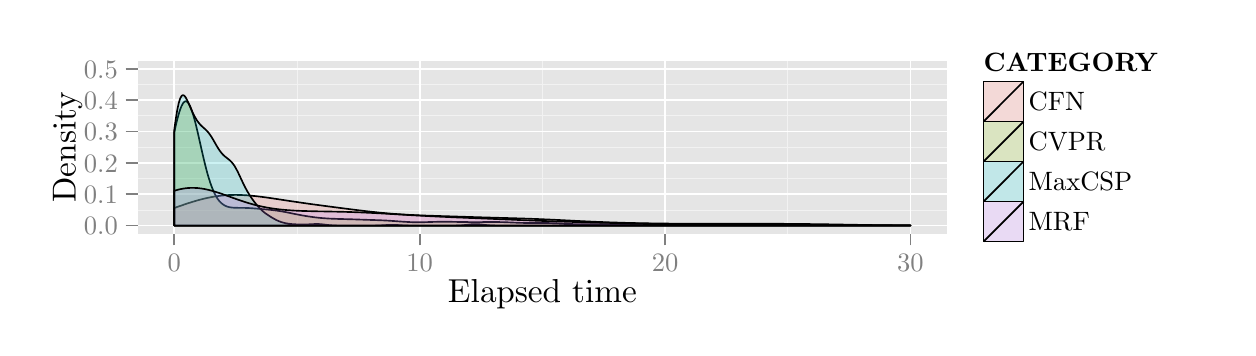
\begin{tikzpicture}[x=1pt,y=1pt]
\definecolor[named]{fillColor}{rgb}{1.00,1.00,1.00}
\path[use as bounding box,fill=fillColor,fill opacity=0.00] (0,0) rectangle (433.62,108.41);
\begin{scope}
\path[clip] (  0.00,  0.00) rectangle (433.62,108.40);
\definecolor[named]{drawColor}{rgb}{1.00,1.00,1.00}
\definecolor[named]{fillColor}{rgb}{1.00,1.00,1.00}

\path[draw=drawColor,line width= 0.6pt,line join=round,line cap=round,fill=fillColor] (  0.00,  0.00) rectangle (433.62,108.40);
\end{scope}
\begin{scope}
\path[clip] ( 39.69, 34.03) rectangle (332.31, 96.36);
\definecolor[named]{fillColor}{rgb}{0.90,0.90,0.90}

\path[fill=fillColor] ( 39.69, 34.03) rectangle (332.31, 96.36);
\definecolor[named]{drawColor}{rgb}{0.95,0.95,0.95}

\path[draw=drawColor,line width= 0.3pt,line join=round] ( 39.69, 42.53) --
	(332.31, 42.53);

\path[draw=drawColor,line width= 0.3pt,line join=round] ( 39.69, 53.87) --
	(332.31, 53.87);

\path[draw=drawColor,line width= 0.3pt,line join=round] ( 39.69, 65.20) --
	(332.31, 65.20);

\path[draw=drawColor,line width= 0.3pt,line join=round] ( 39.69, 76.53) --
	(332.31, 76.53);

\path[draw=drawColor,line width= 0.3pt,line join=round] ( 39.69, 87.86) --
	(332.31, 87.86);

\path[draw=drawColor,line width= 0.3pt,line join=round] ( 97.32, 34.03) --
	( 97.32, 96.36);

\path[draw=drawColor,line width= 0.3pt,line join=round] (186.00, 34.03) --
	(186.00, 96.36);

\path[draw=drawColor,line width= 0.3pt,line join=round] (274.67, 34.03) --
	(274.67, 96.36);
\definecolor[named]{drawColor}{rgb}{1.00,1.00,1.00}

\path[draw=drawColor,line width= 0.6pt,line join=round] ( 39.69, 36.87) --
	(332.31, 36.87);

\path[draw=drawColor,line width= 0.6pt,line join=round] ( 39.69, 48.20) --
	(332.31, 48.20);

\path[draw=drawColor,line width= 0.6pt,line join=round] ( 39.69, 59.53) --
	(332.31, 59.53);

\path[draw=drawColor,line width= 0.6pt,line join=round] ( 39.69, 70.86) --
	(332.31, 70.86);

\path[draw=drawColor,line width= 0.6pt,line join=round] ( 39.69, 82.20) --
	(332.31, 82.20);

\path[draw=drawColor,line width= 0.6pt,line join=round] ( 39.69, 93.53) --
	(332.31, 93.53);

\path[draw=drawColor,line width= 0.6pt,line join=round] ( 52.99, 34.03) --
	( 52.99, 96.36);

\path[draw=drawColor,line width= 0.6pt,line join=round] (141.66, 34.03) --
	(141.66, 96.36);

\path[draw=drawColor,line width= 0.6pt,line join=round] (230.33, 34.03) --
	(230.33, 96.36);

\path[draw=drawColor,line width= 0.6pt,line join=round] (319.00, 34.03) --
	(319.00, 96.36);
\definecolor[named]{drawColor}{rgb}{0.00,0.00,0.00}
\definecolor[named]{fillColor}{rgb}{0.97,0.46,0.43}

\path[draw=drawColor,line width= 0.6pt,line join=round,line cap=round,fill=fillColor,fill opacity=0.20] ( 52.99, 43.26) --
	( 53.51, 43.44) --
	( 54.03, 43.62) --
	( 54.55, 43.80) --
	( 55.07, 43.99) --
	( 55.59, 44.16) --
	( 56.11, 44.34) --
	( 56.63, 44.52) --
	( 57.15, 44.69) --
	( 57.67, 44.87) --
	( 58.19, 45.04) --
	( 58.71, 45.20) --
	( 59.23, 45.37) --
	( 59.75, 45.53) --
	( 60.28, 45.68) --
	( 60.80, 45.84) --
	( 61.32, 45.99) --
	( 61.84, 46.13) --
	( 62.36, 46.27) --
	( 62.88, 46.41) --
	( 63.40, 46.54) --
	( 63.92, 46.66) --
	( 64.44, 46.78) --
	( 64.96, 46.90) --
	( 65.48, 47.01) --
	( 66.00, 47.11) --
	( 66.52, 47.21) --
	( 67.04, 47.30) --
	( 67.56, 47.39) --
	( 68.08, 47.47) --
	( 68.60, 47.54) --
	( 69.13, 47.61) --
	( 69.65, 47.68) --
	( 70.17, 47.73) --
	( 70.69, 47.78) --
	( 71.21, 47.83) --
	( 71.73, 47.87) --
	( 72.25, 47.90) --
	( 72.77, 47.93) --
	( 73.29, 47.95) --
	( 73.81, 47.96) --
	( 74.33, 47.97) --
	( 74.85, 47.98) --
	( 75.37, 47.98) --
	( 75.89, 47.97) --
	( 76.41, 47.96) --
	( 76.93, 47.94) --
	( 77.45, 47.92) --
	( 77.98, 47.90) --
	( 78.50, 47.87) --
	( 79.02, 47.84) --
	( 79.54, 47.80) --
	( 80.06, 47.76) --
	( 80.58, 47.71) --
	( 81.10, 47.67) --
	( 81.62, 47.61) --
	( 82.14, 47.56) --
	( 82.66, 47.50) --
	( 83.18, 47.44) --
	( 83.70, 47.38) --
	( 84.22, 47.32) --
	( 84.74, 47.25) --
	( 85.26, 47.18) --
	( 85.78, 47.11) --
	( 86.30, 47.04) --
	( 86.83, 46.97) --
	( 87.35, 46.89) --
	( 87.87, 46.82) --
	( 88.39, 46.74) --
	( 88.91, 46.66) --
	( 89.43, 46.58) --
	( 89.95, 46.51) --
	( 90.47, 46.43) --
	( 90.99, 46.35) --
	( 91.51, 46.27) --
	( 92.03, 46.19) --
	( 92.55, 46.11) --
	( 93.07, 46.03) --
	( 93.59, 45.95) --
	( 94.11, 45.87) --
	( 94.63, 45.79) --
	( 95.15, 45.72) --
	( 95.68, 45.64) --
	( 96.20, 45.56) --
	( 96.72, 45.48) --
	( 97.24, 45.41) --
	( 97.76, 45.33) --
	( 98.28, 45.25) --
	( 98.80, 45.18) --
	( 99.32, 45.10) --
	( 99.84, 45.03) --
	(100.36, 44.96) --
	(100.88, 44.88) --
	(101.40, 44.81) --
	(101.92, 44.74) --
	(102.44, 44.66) --
	(102.96, 44.59) --
	(103.48, 44.52) --
	(104.00, 44.45) --
	(104.52, 44.38) --
	(105.05, 44.31) --
	(105.57, 44.24) --
	(106.09, 44.17) --
	(106.61, 44.10) --
	(107.13, 44.03) --
	(107.65, 43.96) --
	(108.17, 43.89) --
	(108.69, 43.82) --
	(109.21, 43.76) --
	(109.73, 43.69) --
	(110.25, 43.62) --
	(110.77, 43.55) --
	(111.29, 43.48) --
	(111.81, 43.42) --
	(112.33, 43.35) --
	(112.85, 43.28) --
	(113.37, 43.21) --
	(113.90, 43.15) --
	(114.42, 43.08) --
	(114.94, 43.01) --
	(115.46, 42.95) --
	(115.98, 42.88) --
	(116.50, 42.81) --
	(117.02, 42.75) --
	(117.54, 42.68) --
	(118.06, 42.62) --
	(118.58, 42.55) --
	(119.10, 42.49) --
	(119.62, 42.42) --
	(120.14, 42.36) --
	(120.66, 42.30) --
	(121.18, 42.24) --
	(121.70, 42.17) --
	(122.22, 42.11) --
	(122.75, 42.05) --
	(123.27, 41.99) --
	(123.79, 41.94) --
	(124.31, 41.88) --
	(124.83, 41.82) --
	(125.35, 41.77) --
	(125.87, 41.71) --
	(126.39, 41.66) --
	(126.91, 41.60) --
	(127.43, 41.55) --
	(127.95, 41.50) --
	(128.47, 41.45) --
	(128.99, 41.41) --
	(129.51, 41.36) --
	(130.03, 41.31) --
	(130.55, 41.27) --
	(131.07, 41.23) --
	(131.60, 41.18) --
	(132.12, 41.14) --
	(132.64, 41.10) --
	(133.16, 41.07) --
	(133.68, 41.03) --
	(134.20, 40.99) --
	(134.72, 40.96) --
	(135.24, 40.93) --
	(135.76, 40.89) --
	(136.28, 40.86) --
	(136.80, 40.83) --
	(137.32, 40.80) --
	(137.84, 40.77) --
	(138.36, 40.75) --
	(138.88, 40.72) --
	(139.40, 40.70) --
	(139.92, 40.67) --
	(140.45, 40.65) --
	(140.97, 40.63) --
	(141.49, 40.60) --
	(142.01, 40.58) --
	(142.53, 40.56) --
	(143.05, 40.54) --
	(143.57, 40.52) --
	(144.09, 40.50) --
	(144.61, 40.49) --
	(145.13, 40.47) --
	(145.65, 40.45) --
	(146.17, 40.43) --
	(146.69, 40.42) --
	(147.21, 40.40) --
	(147.73, 40.38) --
	(148.25, 40.37) --
	(148.77, 40.35) --
	(149.29, 40.33) --
	(149.82, 40.32) --
	(150.34, 40.30) --
	(150.86, 40.29) --
	(151.38, 40.27) --
	(151.90, 40.25) --
	(152.42, 40.24) --
	(152.94, 40.22) --
	(153.46, 40.21) --
	(153.98, 40.19) --
	(154.50, 40.17) --
	(155.02, 40.16) --
	(155.54, 40.14) --
	(156.06, 40.13) --
	(156.58, 40.11) --
	(157.10, 40.09) --
	(157.62, 40.08) --
	(158.14, 40.06) --
	(158.67, 40.04) --
	(159.19, 40.03) --
	(159.71, 40.01) --
	(160.23, 39.99) --
	(160.75, 39.98) --
	(161.27, 39.96) --
	(161.79, 39.95) --
	(162.31, 39.93) --
	(162.83, 39.91) --
	(163.35, 39.90) --
	(163.87, 39.88) --
	(164.39, 39.87) --
	(164.91, 39.85) --
	(165.43, 39.84) --
	(165.95, 39.82) --
	(166.47, 39.81) --
	(166.99, 39.79) --
	(167.52, 39.78) --
	(168.04, 39.76) --
	(168.56, 39.75) --
	(169.08, 39.73) --
	(169.60, 39.72) --
	(170.12, 39.70) --
	(170.64, 39.69) --
	(171.16, 39.67) --
	(171.68, 39.66) --
	(172.20, 39.64) --
	(172.72, 39.63) --
	(173.24, 39.62) --
	(173.76, 39.60) --
	(174.28, 39.59) --
	(174.80, 39.57) --
	(175.32, 39.56) --
	(175.84, 39.54) --
	(176.37, 39.53) --
	(176.89, 39.51) --
	(177.41, 39.50) --
	(177.93, 39.48) --
	(178.45, 39.46) --
	(178.97, 39.45) --
	(179.49, 39.43) --
	(180.01, 39.41) --
	(180.53, 39.40) --
	(181.05, 39.38) --
	(181.57, 39.36) --
	(182.09, 39.34) --
	(182.61, 39.32) --
	(183.13, 39.30) --
	(183.65, 39.28) --
	(184.17, 39.26) --
	(184.69, 39.24) --
	(185.22, 39.22) --
	(185.74, 39.20) --
	(186.26, 39.18) --
	(186.78, 39.15) --
	(187.30, 39.13) --
	(187.82, 39.11) --
	(188.34, 39.08) --
	(188.86, 39.06) --
	(189.38, 39.03) --
	(189.90, 39.01) --
	(190.42, 38.99) --
	(190.94, 38.96) --
	(191.46, 38.93) --
	(191.98, 38.91) --
	(192.50, 38.88) --
	(193.02, 38.86) --
	(193.54, 38.83) --
	(194.06, 38.80) --
	(194.59, 38.78) --
	(195.11, 38.75) --
	(195.63, 38.72) --
	(196.15, 38.70) --
	(196.67, 38.67) --
	(197.19, 38.64) --
	(197.71, 38.62) --
	(198.23, 38.59) --
	(198.75, 38.57) --
	(199.27, 38.54) --
	(199.79, 38.51) --
	(200.31, 38.49) --
	(200.83, 38.46) --
	(201.35, 38.44) --
	(201.87, 38.41) --
	(202.39, 38.39) --
	(202.91, 38.37) --
	(203.44, 38.34) --
	(203.96, 38.32) --
	(204.48, 38.30) --
	(205.00, 38.27) --
	(205.52, 38.25) --
	(206.04, 38.23) --
	(206.56, 38.21) --
	(207.08, 38.19) --
	(207.60, 38.17) --
	(208.12, 38.15) --
	(208.64, 38.13) --
	(209.16, 38.11) --
	(209.68, 38.09) --
	(210.20, 38.07) --
	(210.72, 38.05) --
	(211.24, 38.04) --
	(211.76, 38.02) --
	(212.29, 38.00) --
	(212.81, 37.99) --
	(213.33, 37.97) --
	(213.85, 37.95) --
	(214.37, 37.94) --
	(214.89, 37.92) --
	(215.41, 37.91) --
	(215.93, 37.89) --
	(216.45, 37.88) --
	(216.97, 37.87) --
	(217.49, 37.85) --
	(218.01, 37.84) --
	(218.53, 37.83) --
	(219.05, 37.82) --
	(219.57, 37.80) --
	(220.09, 37.79) --
	(220.61, 37.78) --
	(221.14, 37.77) --
	(221.66, 37.76) --
	(222.18, 37.75) --
	(222.70, 37.74) --
	(223.22, 37.73) --
	(223.74, 37.72) --
	(224.26, 37.71) --
	(224.78, 37.70) --
	(225.30, 37.69) --
	(225.82, 37.69) --
	(226.34, 37.68) --
	(226.86, 37.67) --
	(227.38, 37.66) --
	(227.90, 37.66) --
	(228.42, 37.65) --
	(228.94, 37.64) --
	(229.46, 37.64) --
	(229.99, 37.63) --
	(230.51, 37.63) --
	(231.03, 37.62) --
	(231.55, 37.62) --
	(232.07, 37.61) --
	(232.59, 37.61) --
	(233.11, 37.60) --
	(233.63, 37.60) --
	(234.15, 37.60) --
	(234.67, 37.59) --
	(235.19, 37.59) --
	(235.71, 37.59) --
	(236.23, 37.59) --
	(236.75, 37.59) --
	(237.27, 37.59) --
	(237.79, 37.58) --
	(238.31, 37.58) --
	(238.83, 37.58) --
	(239.36, 37.58) --
	(239.88, 37.58) --
	(240.40, 37.58) --
	(240.92, 37.58) --
	(241.44, 37.58) --
	(241.96, 37.58) --
	(242.48, 37.58) --
	(243.00, 37.59) --
	(243.52, 37.59) --
	(244.04, 37.59) --
	(244.56, 37.59) --
	(245.08, 37.59) --
	(245.60, 37.59) --
	(246.12, 37.59) --
	(246.64, 37.59) --
	(247.16, 37.59) --
	(247.68, 37.60) --
	(248.21, 37.60) --
	(248.73, 37.60) --
	(249.25, 37.60) --
	(249.77, 37.60) --
	(250.29, 37.60) --
	(250.81, 37.60) --
	(251.33, 37.60) --
	(251.85, 37.60) --
	(252.37, 37.60) --
	(252.89, 37.60) --
	(253.41, 37.60) --
	(253.93, 37.60) --
	(254.45, 37.60) --
	(254.97, 37.60) --
	(255.49, 37.60) --
	(256.01, 37.60) --
	(256.53, 37.60) --
	(257.06, 37.60) --
	(257.58, 37.60) --
	(258.10, 37.60) --
	(258.62, 37.60) --
	(259.14, 37.60) --
	(259.66, 37.60) --
	(260.18, 37.59) --
	(260.70, 37.59) --
	(261.22, 37.59) --
	(261.74, 37.59) --
	(262.26, 37.59) --
	(262.78, 37.58) --
	(263.30, 37.58) --
	(263.82, 37.58) --
	(264.34, 37.58) --
	(264.86, 37.58) --
	(265.38, 37.57) --
	(265.91, 37.57) --
	(266.43, 37.57) --
	(266.95, 37.56) --
	(267.47, 37.56) --
	(267.99, 37.56) --
	(268.51, 37.56) --
	(269.03, 37.55) --
	(269.55, 37.55) --
	(270.07, 37.55) --
	(270.59, 37.54) --
	(271.11, 37.54) --
	(271.63, 37.54) --
	(272.15, 37.53) --
	(272.67, 37.53) --
	(273.19, 37.53) --
	(273.71, 37.52) --
	(274.23, 37.52) --
	(274.75, 37.51) --
	(275.28, 37.51) --
	(275.80, 37.51) --
	(276.32, 37.50) --
	(276.84, 37.50) --
	(277.36, 37.49) --
	(277.88, 37.49) --
	(278.40, 37.48) --
	(278.92, 37.48) --
	(279.44, 37.47) --
	(279.96, 37.47) --
	(280.48, 37.46) --
	(281.00, 37.46) --
	(281.52, 37.45) --
	(282.04, 37.45) --
	(282.56, 37.44) --
	(283.08, 37.43) --
	(283.60, 37.43) --
	(284.13, 37.42) --
	(284.65, 37.41) --
	(285.17, 37.41) --
	(285.69, 37.40) --
	(286.21, 37.39) --
	(286.73, 37.39) --
	(287.25, 37.38) --
	(287.77, 37.37) --
	(288.29, 37.36) --
	(288.81, 37.35) --
	(289.33, 37.35) --
	(289.85, 37.34) --
	(290.37, 37.33) --
	(290.89, 37.32) --
	(291.41, 37.31) --
	(291.93, 37.30) --
	(292.45, 37.30) --
	(292.98, 37.29) --
	(293.50, 37.28) --
	(294.02, 37.27) --
	(294.54, 37.26) --
	(295.06, 37.25) --
	(295.58, 37.24) --
	(296.10, 37.23) --
	(296.62, 37.22) --
	(297.14, 37.21) --
	(297.66, 37.20) --
	(298.18, 37.20) --
	(298.70, 37.19) --
	(299.22, 37.18) --
	(299.74, 37.17) --
	(300.26, 37.16) --
	(300.78, 37.15) --
	(301.30, 37.14) --
	(301.83, 37.13) --
	(302.35, 37.12) --
	(302.87, 37.12) --
	(303.39, 37.11) --
	(303.91, 37.10) --
	(304.43, 37.09) --
	(304.95, 37.08) --
	(305.47, 37.07) --
	(305.99, 37.07) --
	(306.51, 37.06) --
	(307.03, 37.05) --
	(307.55, 37.04) --
	(308.07, 37.04) --
	(308.59, 37.03) --
	(309.11, 37.02) --
	(309.63, 37.02) --
	(310.15, 37.01) --
	(310.68, 37.00) --
	(311.20, 37.00) --
	(311.72, 36.99) --
	(312.24, 36.99) --
	(312.76, 36.98) --
	(313.28, 36.97) --
	(313.80, 36.97) --
	(314.32, 36.96) --
	(314.84, 36.96) --
	(315.36, 36.95) --
	(315.88, 36.95) --
	(316.40, 36.95) --
	(316.92, 36.94) --
	(317.44, 36.94) --
	(317.96, 36.93) --
	(318.48, 36.93) --
	(319.00, 36.93) --
	(319.00, 36.87) --
	(318.48, 36.87) --
	(317.96, 36.87) --
	(317.44, 36.87) --
	(316.92, 36.87) --
	(316.40, 36.87) --
	(315.88, 36.87) --
	(315.36, 36.87) --
	(314.84, 36.87) --
	(314.32, 36.87) --
	(313.80, 36.87) --
	(313.28, 36.87) --
	(312.76, 36.87) --
	(312.24, 36.87) --
	(311.72, 36.87) --
	(311.20, 36.87) --
	(310.68, 36.87) --
	(310.15, 36.87) --
	(309.63, 36.87) --
	(309.11, 36.87) --
	(308.59, 36.87) --
	(308.07, 36.87) --
	(307.55, 36.87) --
	(307.03, 36.87) --
	(306.51, 36.87) --
	(305.99, 36.87) --
	(305.47, 36.87) --
	(304.95, 36.87) --
	(304.43, 36.87) --
	(303.91, 36.87) --
	(303.39, 36.87) --
	(302.87, 36.87) --
	(302.35, 36.87) --
	(301.83, 36.87) --
	(301.30, 36.87) --
	(300.78, 36.87) --
	(300.26, 36.87) --
	(299.74, 36.87) --
	(299.22, 36.87) --
	(298.70, 36.87) --
	(298.18, 36.87) --
	(297.66, 36.87) --
	(297.14, 36.87) --
	(296.62, 36.87) --
	(296.10, 36.87) --
	(295.58, 36.87) --
	(295.06, 36.87) --
	(294.54, 36.87) --
	(294.02, 36.87) --
	(293.50, 36.87) --
	(292.98, 36.87) --
	(292.45, 36.87) --
	(291.93, 36.87) --
	(291.41, 36.87) --
	(290.89, 36.87) --
	(290.37, 36.87) --
	(289.85, 36.87) --
	(289.33, 36.87) --
	(288.81, 36.87) --
	(288.29, 36.87) --
	(287.77, 36.87) --
	(287.25, 36.87) --
	(286.73, 36.87) --
	(286.21, 36.87) --
	(285.69, 36.87) --
	(285.17, 36.87) --
	(284.65, 36.87) --
	(284.13, 36.87) --
	(283.60, 36.87) --
	(283.08, 36.87) --
	(282.56, 36.87) --
	(282.04, 36.87) --
	(281.52, 36.87) --
	(281.00, 36.87) --
	(280.48, 36.87) --
	(279.96, 36.87) --
	(279.44, 36.87) --
	(278.92, 36.87) --
	(278.40, 36.87) --
	(277.88, 36.87) --
	(277.36, 36.87) --
	(276.84, 36.87) --
	(276.32, 36.87) --
	(275.80, 36.87) --
	(275.28, 36.87) --
	(274.75, 36.87) --
	(274.23, 36.87) --
	(273.71, 36.87) --
	(273.19, 36.87) --
	(272.67, 36.87) --
	(272.15, 36.87) --
	(271.63, 36.87) --
	(271.11, 36.87) --
	(270.59, 36.87) --
	(270.07, 36.87) --
	(269.55, 36.87) --
	(269.03, 36.87) --
	(268.51, 36.87) --
	(267.99, 36.87) --
	(267.47, 36.87) --
	(266.95, 36.87) --
	(266.43, 36.87) --
	(265.91, 36.87) --
	(265.38, 36.87) --
	(264.86, 36.87) --
	(264.34, 36.87) --
	(263.82, 36.87) --
	(263.30, 36.87) --
	(262.78, 36.87) --
	(262.26, 36.87) --
	(261.74, 36.87) --
	(261.22, 36.87) --
	(260.70, 36.87) --
	(260.18, 36.87) --
	(259.66, 36.87) --
	(259.14, 36.87) --
	(258.62, 36.87) --
	(258.10, 36.87) --
	(257.58, 36.87) --
	(257.06, 36.87) --
	(256.53, 36.87) --
	(256.01, 36.87) --
	(255.49, 36.87) --
	(254.97, 36.87) --
	(254.45, 36.87) --
	(253.93, 36.87) --
	(253.41, 36.87) --
	(252.89, 36.87) --
	(252.37, 36.87) --
	(251.85, 36.87) --
	(251.33, 36.87) --
	(250.81, 36.87) --
	(250.29, 36.87) --
	(249.77, 36.87) --
	(249.25, 36.87) --
	(248.73, 36.87) --
	(248.21, 36.87) --
	(247.68, 36.87) --
	(247.16, 36.87) --
	(246.64, 36.87) --
	(246.12, 36.87) --
	(245.60, 36.87) --
	(245.08, 36.87) --
	(244.56, 36.87) --
	(244.04, 36.87) --
	(243.52, 36.87) --
	(243.00, 36.87) --
	(242.48, 36.87) --
	(241.96, 36.87) --
	(241.44, 36.87) --
	(240.92, 36.87) --
	(240.40, 36.87) --
	(239.88, 36.87) --
	(239.36, 36.87) --
	(238.83, 36.87) --
	(238.31, 36.87) --
	(237.79, 36.87) --
	(237.27, 36.87) --
	(236.75, 36.87) --
	(236.23, 36.87) --
	(235.71, 36.87) --
	(235.19, 36.87) --
	(234.67, 36.87) --
	(234.15, 36.87) --
	(233.63, 36.87) --
	(233.11, 36.87) --
	(232.59, 36.87) --
	(232.07, 36.87) --
	(231.55, 36.87) --
	(231.03, 36.87) --
	(230.51, 36.87) --
	(229.99, 36.87) --
	(229.46, 36.87) --
	(228.94, 36.87) --
	(228.42, 36.87) --
	(227.90, 36.87) --
	(227.38, 36.87) --
	(226.86, 36.87) --
	(226.34, 36.87) --
	(225.82, 36.87) --
	(225.30, 36.87) --
	(224.78, 36.87) --
	(224.26, 36.87) --
	(223.74, 36.87) --
	(223.22, 36.87) --
	(222.70, 36.87) --
	(222.18, 36.87) --
	(221.66, 36.87) --
	(221.14, 36.87) --
	(220.61, 36.87) --
	(220.09, 36.87) --
	(219.57, 36.87) --
	(219.05, 36.87) --
	(218.53, 36.87) --
	(218.01, 36.87) --
	(217.49, 36.87) --
	(216.97, 36.87) --
	(216.45, 36.87) --
	(215.93, 36.87) --
	(215.41, 36.87) --
	(214.89, 36.87) --
	(214.37, 36.87) --
	(213.85, 36.87) --
	(213.33, 36.87) --
	(212.81, 36.87) --
	(212.29, 36.87) --
	(211.76, 36.87) --
	(211.24, 36.87) --
	(210.72, 36.87) --
	(210.20, 36.87) --
	(209.68, 36.87) --
	(209.16, 36.87) --
	(208.64, 36.87) --
	(208.12, 36.87) --
	(207.60, 36.87) --
	(207.08, 36.87) --
	(206.56, 36.87) --
	(206.04, 36.87) --
	(205.52, 36.87) --
	(205.00, 36.87) --
	(204.48, 36.87) --
	(203.96, 36.87) --
	(203.44, 36.87) --
	(202.91, 36.87) --
	(202.39, 36.87) --
	(201.87, 36.87) --
	(201.35, 36.87) --
	(200.83, 36.87) --
	(200.31, 36.87) --
	(199.79, 36.87) --
	(199.27, 36.87) --
	(198.75, 36.87) --
	(198.23, 36.87) --
	(197.71, 36.87) --
	(197.19, 36.87) --
	(196.67, 36.87) --
	(196.15, 36.87) --
	(195.63, 36.87) --
	(195.11, 36.87) --
	(194.59, 36.87) --
	(194.06, 36.87) --
	(193.54, 36.87) --
	(193.02, 36.87) --
	(192.50, 36.87) --
	(191.98, 36.87) --
	(191.46, 36.87) --
	(190.94, 36.87) --
	(190.42, 36.87) --
	(189.90, 36.87) --
	(189.38, 36.87) --
	(188.86, 36.87) --
	(188.34, 36.87) --
	(187.82, 36.87) --
	(187.30, 36.87) --
	(186.78, 36.87) --
	(186.26, 36.87) --
	(185.74, 36.87) --
	(185.22, 36.87) --
	(184.69, 36.87) --
	(184.17, 36.87) --
	(183.65, 36.87) --
	(183.13, 36.87) --
	(182.61, 36.87) --
	(182.09, 36.87) --
	(181.57, 36.87) --
	(181.05, 36.87) --
	(180.53, 36.87) --
	(180.01, 36.87) --
	(179.49, 36.87) --
	(178.97, 36.87) --
	(178.45, 36.87) --
	(177.93, 36.87) --
	(177.41, 36.87) --
	(176.89, 36.87) --
	(176.37, 36.87) --
	(175.84, 36.87) --
	(175.32, 36.87) --
	(174.80, 36.87) --
	(174.28, 36.87) --
	(173.76, 36.87) --
	(173.24, 36.87) --
	(172.72, 36.87) --
	(172.20, 36.87) --
	(171.68, 36.87) --
	(171.16, 36.87) --
	(170.64, 36.87) --
	(170.12, 36.87) --
	(169.60, 36.87) --
	(169.08, 36.87) --
	(168.56, 36.87) --
	(168.04, 36.87) --
	(167.52, 36.87) --
	(166.99, 36.87) --
	(166.47, 36.87) --
	(165.95, 36.87) --
	(165.43, 36.87) --
	(164.91, 36.87) --
	(164.39, 36.87) --
	(163.87, 36.87) --
	(163.35, 36.87) --
	(162.83, 36.87) --
	(162.31, 36.87) --
	(161.79, 36.87) --
	(161.27, 36.87) --
	(160.75, 36.87) --
	(160.23, 36.87) --
	(159.71, 36.87) --
	(159.19, 36.87) --
	(158.67, 36.87) --
	(158.14, 36.87) --
	(157.62, 36.87) --
	(157.10, 36.87) --
	(156.58, 36.87) --
	(156.06, 36.87) --
	(155.54, 36.87) --
	(155.02, 36.87) --
	(154.50, 36.87) --
	(153.98, 36.87) --
	(153.46, 36.87) --
	(152.94, 36.87) --
	(152.42, 36.87) --
	(151.90, 36.87) --
	(151.38, 36.87) --
	(150.86, 36.87) --
	(150.34, 36.87) --
	(149.82, 36.87) --
	(149.29, 36.87) --
	(148.77, 36.87) --
	(148.25, 36.87) --
	(147.73, 36.87) --
	(147.21, 36.87) --
	(146.69, 36.87) --
	(146.17, 36.87) --
	(145.65, 36.87) --
	(145.13, 36.87) --
	(144.61, 36.87) --
	(144.09, 36.87) --
	(143.57, 36.87) --
	(143.05, 36.87) --
	(142.53, 36.87) --
	(142.01, 36.87) --
	(141.49, 36.87) --
	(140.97, 36.87) --
	(140.45, 36.87) --
	(139.92, 36.87) --
	(139.40, 36.87) --
	(138.88, 36.87) --
	(138.36, 36.87) --
	(137.84, 36.87) --
	(137.32, 36.87) --
	(136.80, 36.87) --
	(136.28, 36.87) --
	(135.76, 36.87) --
	(135.24, 36.87) --
	(134.72, 36.87) --
	(134.20, 36.87) --
	(133.68, 36.87) --
	(133.16, 36.87) --
	(132.64, 36.87) --
	(132.12, 36.87) --
	(131.60, 36.87) --
	(131.07, 36.87) --
	(130.55, 36.87) --
	(130.03, 36.87) --
	(129.51, 36.87) --
	(128.99, 36.87) --
	(128.47, 36.87) --
	(127.95, 36.87) --
	(127.43, 36.87) --
	(126.91, 36.87) --
	(126.39, 36.87) --
	(125.87, 36.87) --
	(125.35, 36.87) --
	(124.83, 36.87) --
	(124.31, 36.87) --
	(123.79, 36.87) --
	(123.27, 36.87) --
	(122.75, 36.87) --
	(122.22, 36.87) --
	(121.70, 36.87) --
	(121.18, 36.87) --
	(120.66, 36.87) --
	(120.14, 36.87) --
	(119.62, 36.87) --
	(119.10, 36.87) --
	(118.58, 36.87) --
	(118.06, 36.87) --
	(117.54, 36.87) --
	(117.02, 36.87) --
	(116.50, 36.87) --
	(115.98, 36.87) --
	(115.46, 36.87) --
	(114.94, 36.87) --
	(114.42, 36.87) --
	(113.90, 36.87) --
	(113.37, 36.87) --
	(112.85, 36.87) --
	(112.33, 36.87) --
	(111.81, 36.87) --
	(111.29, 36.87) --
	(110.77, 36.87) --
	(110.25, 36.87) --
	(109.73, 36.87) --
	(109.21, 36.87) --
	(108.69, 36.87) --
	(108.17, 36.87) --
	(107.65, 36.87) --
	(107.13, 36.87) --
	(106.61, 36.87) --
	(106.09, 36.87) --
	(105.57, 36.87) --
	(105.05, 36.87) --
	(104.52, 36.87) --
	(104.00, 36.87) --
	(103.48, 36.87) --
	(102.96, 36.87) --
	(102.44, 36.87) --
	(101.92, 36.87) --
	(101.40, 36.87) --
	(100.88, 36.87) --
	(100.36, 36.87) --
	( 99.84, 36.87) --
	( 99.32, 36.87) --
	( 98.80, 36.87) --
	( 98.28, 36.87) --
	( 97.76, 36.87) --
	( 97.24, 36.87) --
	( 96.72, 36.87) --
	( 96.20, 36.87) --
	( 95.68, 36.87) --
	( 95.15, 36.87) --
	( 94.63, 36.87) --
	( 94.11, 36.87) --
	( 93.59, 36.87) --
	( 93.07, 36.87) --
	( 92.55, 36.87) --
	( 92.03, 36.87) --
	( 91.51, 36.87) --
	( 90.99, 36.87) --
	( 90.47, 36.87) --
	( 89.95, 36.87) --
	( 89.43, 36.87) --
	( 88.91, 36.87) --
	( 88.39, 36.87) --
	( 87.87, 36.87) --
	( 87.35, 36.87) --
	( 86.83, 36.87) --
	( 86.30, 36.87) --
	( 85.78, 36.87) --
	( 85.26, 36.87) --
	( 84.74, 36.87) --
	( 84.22, 36.87) --
	( 83.70, 36.87) --
	( 83.18, 36.87) --
	( 82.66, 36.87) --
	( 82.14, 36.87) --
	( 81.62, 36.87) --
	( 81.10, 36.87) --
	( 80.58, 36.87) --
	( 80.06, 36.87) --
	( 79.54, 36.87) --
	( 79.02, 36.87) --
	( 78.50, 36.87) --
	( 77.98, 36.87) --
	( 77.45, 36.87) --
	( 76.93, 36.87) --
	( 76.41, 36.87) --
	( 75.89, 36.87) --
	( 75.37, 36.87) --
	( 74.85, 36.87) --
	( 74.33, 36.87) --
	( 73.81, 36.87) --
	( 73.29, 36.87) --
	( 72.77, 36.87) --
	( 72.25, 36.87) --
	( 71.73, 36.87) --
	( 71.21, 36.87) --
	( 70.69, 36.87) --
	( 70.17, 36.87) --
	( 69.65, 36.87) --
	( 69.13, 36.87) --
	( 68.60, 36.87) --
	( 68.08, 36.87) --
	( 67.56, 36.87) --
	( 67.04, 36.87) --
	( 66.52, 36.87) --
	( 66.00, 36.87) --
	( 65.48, 36.87) --
	( 64.96, 36.87) --
	( 64.44, 36.87) --
	( 63.92, 36.87) --
	( 63.40, 36.87) --
	( 62.88, 36.87) --
	( 62.36, 36.87) --
	( 61.84, 36.87) --
	( 61.32, 36.87) --
	( 60.80, 36.87) --
	( 60.28, 36.87) --
	( 59.75, 36.87) --
	( 59.23, 36.87) --
	( 58.71, 36.87) --
	( 58.19, 36.87) --
	( 57.67, 36.87) --
	( 57.15, 36.87) --
	( 56.63, 36.87) --
	( 56.11, 36.87) --
	( 55.59, 36.87) --
	( 55.07, 36.87) --
	( 54.55, 36.87) --
	( 54.03, 36.87) --
	( 53.51, 36.87) --
	( 52.99, 36.87) --
	cycle;
\definecolor[named]{fillColor}{rgb}{0.49,0.68,0.00}

\path[draw=drawColor,line width= 0.6pt,line join=round,line cap=round,fill=fillColor,fill opacity=0.20] ( 52.99, 70.61) --
	( 53.51, 73.00) --
	( 54.03, 75.18) --
	( 54.55, 77.11) --
	( 55.07, 78.76) --
	( 55.59, 80.08) --
	( 56.11, 81.05) --
	( 56.63, 81.64) --
	( 57.15, 81.85) --
	( 57.67, 81.60) --
	( 58.19, 80.97) --
	( 58.71, 79.99) --
	( 59.23, 78.69) --
	( 59.75, 77.11) --
	( 60.28, 75.28) --
	( 60.80, 73.25) --
	( 61.32, 71.07) --
	( 61.84, 68.79) --
	( 62.36, 66.48) --
	( 62.88, 64.17) --
	( 63.40, 61.91) --
	( 63.92, 59.73) --
	( 64.44, 57.65) --
	( 64.96, 55.71) --
	( 65.48, 53.93) --
	( 66.00, 52.32) --
	( 66.52, 50.87) --
	( 67.04, 49.58) --
	( 67.56, 48.45) --
	( 68.08, 47.46) --
	( 68.60, 46.62) --
	( 69.13, 45.91) --
	( 69.65, 45.33) --
	( 70.17, 44.86) --
	( 70.69, 44.47) --
	( 71.21, 44.16) --
	( 71.73, 43.91) --
	( 72.25, 43.72) --
	( 72.77, 43.58) --
	( 73.29, 43.48) --
	( 73.81, 43.41) --
	( 74.33, 43.37) --
	( 74.85, 43.34) --
	( 75.37, 43.32) --
	( 75.89, 43.31) --
	( 76.41, 43.30) --
	( 76.93, 43.30) --
	( 77.45, 43.30) --
	( 77.98, 43.29) --
	( 78.50, 43.28) --
	( 79.02, 43.26) --
	( 79.54, 43.24) --
	( 80.06, 43.22) --
	( 80.58, 43.19) --
	( 81.10, 43.15) --
	( 81.62, 43.12) --
	( 82.14, 43.07) --
	( 82.66, 43.03) --
	( 83.18, 42.99) --
	( 83.70, 42.94) --
	( 84.22, 42.89) --
	( 84.74, 42.85) --
	( 85.26, 42.80) --
	( 85.78, 42.76) --
	( 86.30, 42.71) --
	( 86.83, 42.66) --
	( 87.35, 42.61) --
	( 87.87, 42.56) --
	( 88.39, 42.50) --
	( 88.91, 42.44) --
	( 89.43, 42.38) --
	( 89.95, 42.31) --
	( 90.47, 42.23) --
	( 90.99, 42.15) --
	( 91.51, 42.07) --
	( 92.03, 41.98) --
	( 92.55, 41.89) --
	( 93.07, 41.79) --
	( 93.59, 41.69) --
	( 94.11, 41.58) --
	( 94.63, 41.48) --
	( 95.15, 41.37) --
	( 95.68, 41.26) --
	( 96.20, 41.16) --
	( 96.72, 41.05) --
	( 97.24, 40.95) --
	( 97.76, 40.85) --
	( 98.28, 40.75) --
	( 98.80, 40.65) --
	( 99.32, 40.56) --
	( 99.84, 40.47) --
	(100.36, 40.38) --
	(100.88, 40.29) --
	(101.40, 40.21) --
	(101.92, 40.14) --
	(102.44, 40.06) --
	(102.96, 39.99) --
	(103.48, 39.92) --
	(104.00, 39.85) --
	(104.52, 39.79) --
	(105.05, 39.74) --
	(105.57, 39.68) --
	(106.09, 39.63) --
	(106.61, 39.59) --
	(107.13, 39.55) --
	(107.65, 39.51) --
	(108.17, 39.47) --
	(108.69, 39.44) --
	(109.21, 39.41) --
	(109.73, 39.39) --
	(110.25, 39.37) --
	(110.77, 39.35) --
	(111.29, 39.33) --
	(111.81, 39.31) --
	(112.33, 39.29) --
	(112.85, 39.28) --
	(113.37, 39.26) --
	(113.90, 39.25) --
	(114.42, 39.24) --
	(114.94, 39.22) --
	(115.46, 39.21) --
	(115.98, 39.20) --
	(116.50, 39.18) --
	(117.02, 39.17) --
	(117.54, 39.15) --
	(118.06, 39.13) --
	(118.58, 39.12) --
	(119.10, 39.10) --
	(119.62, 39.08) --
	(120.14, 39.06) --
	(120.66, 39.04) --
	(121.18, 39.03) --
	(121.70, 39.01) --
	(122.22, 38.99) --
	(122.75, 38.97) --
	(123.27, 38.95) --
	(123.79, 38.94) --
	(124.31, 38.92) --
	(124.83, 38.90) --
	(125.35, 38.89) --
	(125.87, 38.87) --
	(126.39, 38.85) --
	(126.91, 38.83) --
	(127.43, 38.81) --
	(127.95, 38.79) --
	(128.47, 38.77) --
	(128.99, 38.74) --
	(129.51, 38.72) --
	(130.03, 38.69) --
	(130.55, 38.66) --
	(131.07, 38.62) --
	(131.60, 38.59) --
	(132.12, 38.55) --
	(132.64, 38.52) --
	(133.16, 38.48) --
	(133.68, 38.44) --
	(134.20, 38.40) --
	(134.72, 38.36) --
	(135.24, 38.33) --
	(135.76, 38.29) --
	(136.28, 38.26) --
	(136.80, 38.23) --
	(137.32, 38.20) --
	(137.84, 38.17) --
	(138.36, 38.15) --
	(138.88, 38.13) --
	(139.40, 38.11) --
	(139.92, 38.10) --
	(140.45, 38.09) --
	(140.97, 38.09) --
	(141.49, 38.09) --
	(142.01, 38.10) --
	(142.53, 38.10) --
	(143.05, 38.11) --
	(143.57, 38.13) --
	(144.09, 38.14) --
	(144.61, 38.16) --
	(145.13, 38.18) --
	(145.65, 38.19) --
	(146.17, 38.21) --
	(146.69, 38.23) --
	(147.21, 38.24) --
	(147.73, 38.25) --
	(148.25, 38.26) --
	(148.77, 38.27) --
	(149.29, 38.28) --
	(149.82, 38.28) --
	(150.34, 38.28) --
	(150.86, 38.28) --
	(151.38, 38.28) --
	(151.90, 38.27) --
	(152.42, 38.26) --
	(152.94, 38.26) --
	(153.46, 38.25) --
	(153.98, 38.24) --
	(154.50, 38.23) --
	(155.02, 38.22) --
	(155.54, 38.21) --
	(156.06, 38.20) --
	(156.58, 38.20) --
	(157.10, 38.19) --
	(157.62, 38.18) --
	(158.14, 38.17) --
	(158.67, 38.17) --
	(159.19, 38.16) --
	(159.71, 38.16) --
	(160.23, 38.16) --
	(160.75, 38.16) --
	(161.27, 38.15) --
	(161.79, 38.15) --
	(162.31, 38.15) --
	(162.83, 38.16) --
	(163.35, 38.16) --
	(163.87, 38.16) --
	(164.39, 38.16) --
	(164.91, 38.17) --
	(165.43, 38.17) --
	(165.95, 38.18) --
	(166.47, 38.18) --
	(166.99, 38.18) --
	(167.52, 38.19) --
	(168.04, 38.19) --
	(168.56, 38.19) --
	(169.08, 38.18) --
	(169.60, 38.18) --
	(170.12, 38.17) --
	(170.64, 38.16) --
	(171.16, 38.15) --
	(171.68, 38.14) --
	(172.20, 38.12) --
	(172.72, 38.11) --
	(173.24, 38.09) --
	(173.76, 38.06) --
	(174.28, 38.04) --
	(174.80, 38.02) --
	(175.32, 37.99) --
	(175.84, 37.97) --
	(176.37, 37.95) --
	(176.89, 37.93) --
	(177.41, 37.91) --
	(177.93, 37.89) --
	(178.45, 37.87) --
	(178.97, 37.86) --
	(179.49, 37.85) --
	(180.01, 37.84) --
	(180.53, 37.83) --
	(181.05, 37.82) --
	(181.57, 37.82) --
	(182.09, 37.81) --
	(182.61, 37.81) --
	(183.13, 37.81) --
	(183.65, 37.81) --
	(184.17, 37.81) --
	(184.69, 37.81) --
	(185.22, 37.82) --
	(185.74, 37.82) --
	(186.26, 37.81) --
	(186.78, 37.81) --
	(187.30, 37.81) --
	(187.82, 37.80) --
	(188.34, 37.80) --
	(188.86, 37.79) --
	(189.38, 37.77) --
	(189.90, 37.76) --
	(190.42, 37.74) --
	(190.94, 37.72) --
	(191.46, 37.70) --
	(191.98, 37.68) --
	(192.50, 37.65) --
	(193.02, 37.63) --
	(193.54, 37.60) --
	(194.06, 37.57) --
	(194.59, 37.55) --
	(195.11, 37.52) --
	(195.63, 37.50) --
	(196.15, 37.48) --
	(196.67, 37.45) --
	(197.19, 37.43) --
	(197.71, 37.42) --
	(198.23, 37.40) --
	(198.75, 37.39) --
	(199.27, 37.38) --
	(199.79, 37.37) --
	(200.31, 37.37) --
	(200.83, 37.37) --
	(201.35, 37.36) --
	(201.87, 37.36) --
	(202.39, 37.37) --
	(202.91, 37.37) --
	(203.44, 37.37) --
	(203.96, 37.37) --
	(204.48, 37.38) --
	(205.00, 37.38) --
	(205.52, 37.38) --
	(206.04, 37.39) --
	(206.56, 37.39) --
	(207.08, 37.39) --
	(207.60, 37.39) --
	(208.12, 37.39) --
	(208.64, 37.39) --
	(209.16, 37.39) --
	(209.68, 37.38) --
	(210.20, 37.38) --
	(210.72, 37.38) --
	(211.24, 37.37) --
	(211.76, 37.37) --
	(212.29, 37.36) --
	(212.81, 37.36) --
	(213.33, 37.35) --
	(213.85, 37.34) --
	(214.37, 37.34) --
	(214.89, 37.33) --
	(215.41, 37.32) --
	(215.93, 37.31) --
	(216.45, 37.31) --
	(216.97, 37.30) --
	(217.49, 37.29) --
	(218.01, 37.29) --
	(218.53, 37.29) --
	(219.05, 37.28) --
	(219.57, 37.28) --
	(220.09, 37.28) --
	(220.61, 37.28) --
	(221.14, 37.28) --
	(221.66, 37.28) --
	(222.18, 37.28) --
	(222.70, 37.29) --
	(223.22, 37.29) --
	(223.74, 37.30) --
	(224.26, 37.30) --
	(224.78, 37.30) --
	(225.30, 37.31) --
	(225.82, 37.31) --
	(226.34, 37.32) --
	(226.86, 37.32) --
	(227.38, 37.33) --
	(227.90, 37.33) --
	(228.42, 37.33) --
	(228.94, 37.34) --
	(229.46, 37.34) --
	(229.99, 37.34) --
	(230.51, 37.35) --
	(231.03, 37.35) --
	(231.55, 37.36) --
	(232.07, 37.36) --
	(232.59, 37.37) --
	(233.11, 37.38) --
	(233.63, 37.38) --
	(234.15, 37.39) --
	(234.67, 37.40) --
	(235.19, 37.40) --
	(235.71, 37.41) --
	(236.23, 37.42) --
	(236.75, 37.42) --
	(237.27, 37.42) --
	(237.79, 37.42) --
	(238.31, 37.42) --
	(238.83, 37.41) --
	(239.36, 37.40) --
	(239.88, 37.39) --
	(240.40, 37.38) --
	(240.92, 37.36) --
	(241.44, 37.35) --
	(241.96, 37.33) --
	(242.48, 37.31) --
	(243.00, 37.29) --
	(243.52, 37.26) --
	(244.04, 37.24) --
	(244.56, 37.22) --
	(245.08, 37.20) --
	(245.60, 37.19) --
	(246.12, 37.17) --
	(246.64, 37.16) --
	(247.16, 37.15) --
	(247.68, 37.15) --
	(248.21, 37.14) --
	(248.73, 37.15) --
	(249.25, 37.15) --
	(249.77, 37.16) --
	(250.29, 37.17) --
	(250.81, 37.18) --
	(251.33, 37.20) --
	(251.85, 37.21) --
	(252.37, 37.23) --
	(252.89, 37.25) --
	(253.41, 37.26) --
	(253.93, 37.28) --
	(254.45, 37.30) --
	(254.97, 37.31) --
	(255.49, 37.33) --
	(256.01, 37.34) --
	(256.53, 37.35) --
	(257.06, 37.35) --
	(257.58, 37.36) --
	(258.10, 37.36) --
	(258.62, 37.35) --
	(259.14, 37.35) --
	(259.66, 37.35) --
	(260.18, 37.34) --
	(260.70, 37.33) --
	(261.22, 37.32) --
	(261.74, 37.31) --
	(262.26, 37.30) --
	(262.78, 37.29) --
	(263.30, 37.28) --
	(263.82, 37.27) --
	(264.34, 37.26) --
	(264.86, 37.25) --
	(265.38, 37.25) --
	(265.91, 37.25) --
	(266.43, 37.25) --
	(266.95, 37.25) --
	(267.47, 37.25) --
	(267.99, 37.25) --
	(268.51, 37.26) --
	(269.03, 37.27) --
	(269.55, 37.28) --
	(270.07, 37.29) --
	(270.59, 37.30) --
	(271.11, 37.31) --
	(271.63, 37.32) --
	(272.15, 37.33) --
	(272.67, 37.34) --
	(273.19, 37.35) --
	(273.71, 37.36) --
	(274.23, 37.36) --
	(274.75, 37.36) --
	(275.28, 37.36) --
	(275.80, 37.36) --
	(276.32, 37.36) --
	(276.84, 37.35) --
	(277.36, 37.34) --
	(277.88, 37.33) --
	(278.40, 37.31) --
	(278.92, 37.30) --
	(279.44, 37.28) --
	(279.96, 37.27) --
	(280.48, 37.25) --
	(281.00, 37.23) --
	(281.52, 37.22) --
	(282.04, 37.20) --
	(282.56, 37.18) --
	(283.08, 37.17) --
	(283.60, 37.16) --
	(284.13, 37.14) --
	(284.65, 37.13) --
	(285.17, 37.12) --
	(285.69, 37.11) --
	(286.21, 37.10) --
	(286.73, 37.10) --
	(287.25, 37.09) --
	(287.77, 37.08) --
	(288.29, 37.08) --
	(288.81, 37.07) --
	(289.33, 37.07) --
	(289.85, 37.06) --
	(290.37, 37.06) --
	(290.89, 37.06) --
	(291.41, 37.05) --
	(291.93, 37.05) --
	(292.45, 37.05) --
	(292.98, 37.05) --
	(293.50, 37.04) --
	(294.02, 37.04) --
	(294.54, 37.04) --
	(295.06, 37.04) --
	(295.58, 37.04) --
	(296.10, 37.04) --
	(296.62, 37.03) --
	(297.14, 37.03) --
	(297.66, 37.03) --
	(298.18, 37.03) --
	(298.70, 37.03) --
	(299.22, 37.03) --
	(299.74, 37.03) --
	(300.26, 37.03) --
	(300.78, 37.03) --
	(301.30, 37.03) --
	(301.83, 37.03) --
	(302.35, 37.03) --
	(302.87, 37.02) --
	(303.39, 37.02) --
	(303.91, 37.02) --
	(304.43, 37.02) --
	(304.95, 37.02) --
	(305.47, 37.02) --
	(305.99, 37.02) --
	(306.51, 37.02) --
	(307.03, 37.02) --
	(307.55, 37.02) --
	(308.07, 37.02) --
	(308.59, 37.02) --
	(309.11, 37.02) --
	(309.63, 37.02) --
	(310.15, 37.02) --
	(310.68, 37.02) --
	(311.20, 37.02) --
	(311.72, 37.02) --
	(312.24, 37.02) --
	(312.76, 37.02) --
	(313.28, 37.02) --
	(313.80, 37.02) --
	(314.32, 37.02) --
	(314.84, 37.02) --
	(315.36, 37.02) --
	(315.88, 37.02) --
	(316.40, 37.02) --
	(316.92, 37.01) --
	(317.44, 37.01) --
	(317.96, 37.00) --
	(318.48, 36.99) --
	(319.00, 36.99) --
	(319.00, 36.87) --
	(318.48, 36.87) --
	(317.96, 36.87) --
	(317.44, 36.87) --
	(316.92, 36.87) --
	(316.40, 36.87) --
	(315.88, 36.87) --
	(315.36, 36.87) --
	(314.84, 36.87) --
	(314.32, 36.87) --
	(313.80, 36.87) --
	(313.28, 36.87) --
	(312.76, 36.87) --
	(312.24, 36.87) --
	(311.72, 36.87) --
	(311.20, 36.87) --
	(310.68, 36.87) --
	(310.15, 36.87) --
	(309.63, 36.87) --
	(309.11, 36.87) --
	(308.59, 36.87) --
	(308.07, 36.87) --
	(307.55, 36.87) --
	(307.03, 36.87) --
	(306.51, 36.87) --
	(305.99, 36.87) --
	(305.47, 36.87) --
	(304.95, 36.87) --
	(304.43, 36.87) --
	(303.91, 36.87) --
	(303.39, 36.87) --
	(302.87, 36.87) --
	(302.35, 36.87) --
	(301.83, 36.87) --
	(301.30, 36.87) --
	(300.78, 36.87) --
	(300.26, 36.87) --
	(299.74, 36.87) --
	(299.22, 36.87) --
	(298.70, 36.87) --
	(298.18, 36.87) --
	(297.66, 36.87) --
	(297.14, 36.87) --
	(296.62, 36.87) --
	(296.10, 36.87) --
	(295.58, 36.87) --
	(295.06, 36.87) --
	(294.54, 36.87) --
	(294.02, 36.87) --
	(293.50, 36.87) --
	(292.98, 36.87) --
	(292.45, 36.87) --
	(291.93, 36.87) --
	(291.41, 36.87) --
	(290.89, 36.87) --
	(290.37, 36.87) --
	(289.85, 36.87) --
	(289.33, 36.87) --
	(288.81, 36.87) --
	(288.29, 36.87) --
	(287.77, 36.87) --
	(287.25, 36.87) --
	(286.73, 36.87) --
	(286.21, 36.87) --
	(285.69, 36.87) --
	(285.17, 36.87) --
	(284.65, 36.87) --
	(284.13, 36.87) --
	(283.60, 36.87) --
	(283.08, 36.87) --
	(282.56, 36.87) --
	(282.04, 36.87) --
	(281.52, 36.87) --
	(281.00, 36.87) --
	(280.48, 36.87) --
	(279.96, 36.87) --
	(279.44, 36.87) --
	(278.92, 36.87) --
	(278.40, 36.87) --
	(277.88, 36.87) --
	(277.36, 36.87) --
	(276.84, 36.87) --
	(276.32, 36.87) --
	(275.80, 36.87) --
	(275.28, 36.87) --
	(274.75, 36.87) --
	(274.23, 36.87) --
	(273.71, 36.87) --
	(273.19, 36.87) --
	(272.67, 36.87) --
	(272.15, 36.87) --
	(271.63, 36.87) --
	(271.11, 36.87) --
	(270.59, 36.87) --
	(270.07, 36.87) --
	(269.55, 36.87) --
	(269.03, 36.87) --
	(268.51, 36.87) --
	(267.99, 36.87) --
	(267.47, 36.87) --
	(266.95, 36.87) --
	(266.43, 36.87) --
	(265.91, 36.87) --
	(265.38, 36.87) --
	(264.86, 36.87) --
	(264.34, 36.87) --
	(263.82, 36.87) --
	(263.30, 36.87) --
	(262.78, 36.87) --
	(262.26, 36.87) --
	(261.74, 36.87) --
	(261.22, 36.87) --
	(260.70, 36.87) --
	(260.18, 36.87) --
	(259.66, 36.87) --
	(259.14, 36.87) --
	(258.62, 36.87) --
	(258.10, 36.87) --
	(257.58, 36.87) --
	(257.06, 36.87) --
	(256.53, 36.87) --
	(256.01, 36.87) --
	(255.49, 36.87) --
	(254.97, 36.87) --
	(254.45, 36.87) --
	(253.93, 36.87) --
	(253.41, 36.87) --
	(252.89, 36.87) --
	(252.37, 36.87) --
	(251.85, 36.87) --
	(251.33, 36.87) --
	(250.81, 36.87) --
	(250.29, 36.87) --
	(249.77, 36.87) --
	(249.25, 36.87) --
	(248.73, 36.87) --
	(248.21, 36.87) --
	(247.68, 36.87) --
	(247.16, 36.87) --
	(246.64, 36.87) --
	(246.12, 36.87) --
	(245.60, 36.87) --
	(245.08, 36.87) --
	(244.56, 36.87) --
	(244.04, 36.87) --
	(243.52, 36.87) --
	(243.00, 36.87) --
	(242.48, 36.87) --
	(241.96, 36.87) --
	(241.44, 36.87) --
	(240.92, 36.87) --
	(240.40, 36.87) --
	(239.88, 36.87) --
	(239.36, 36.87) --
	(238.83, 36.87) --
	(238.31, 36.87) --
	(237.79, 36.87) --
	(237.27, 36.87) --
	(236.75, 36.87) --
	(236.23, 36.87) --
	(235.71, 36.87) --
	(235.19, 36.87) --
	(234.67, 36.87) --
	(234.15, 36.87) --
	(233.63, 36.87) --
	(233.11, 36.87) --
	(232.59, 36.87) --
	(232.07, 36.87) --
	(231.55, 36.87) --
	(231.03, 36.87) --
	(230.51, 36.87) --
	(229.99, 36.87) --
	(229.46, 36.87) --
	(228.94, 36.87) --
	(228.42, 36.87) --
	(227.90, 36.87) --
	(227.38, 36.87) --
	(226.86, 36.87) --
	(226.34, 36.87) --
	(225.82, 36.87) --
	(225.30, 36.87) --
	(224.78, 36.87) --
	(224.26, 36.87) --
	(223.74, 36.87) --
	(223.22, 36.87) --
	(222.70, 36.87) --
	(222.18, 36.87) --
	(221.66, 36.87) --
	(221.14, 36.87) --
	(220.61, 36.87) --
	(220.09, 36.87) --
	(219.57, 36.87) --
	(219.05, 36.87) --
	(218.53, 36.87) --
	(218.01, 36.87) --
	(217.49, 36.87) --
	(216.97, 36.87) --
	(216.45, 36.87) --
	(215.93, 36.87) --
	(215.41, 36.87) --
	(214.89, 36.87) --
	(214.37, 36.87) --
	(213.85, 36.87) --
	(213.33, 36.87) --
	(212.81, 36.87) --
	(212.29, 36.87) --
	(211.76, 36.87) --
	(211.24, 36.87) --
	(210.72, 36.87) --
	(210.20, 36.87) --
	(209.68, 36.87) --
	(209.16, 36.87) --
	(208.64, 36.87) --
	(208.12, 36.87) --
	(207.60, 36.87) --
	(207.08, 36.87) --
	(206.56, 36.87) --
	(206.04, 36.87) --
	(205.52, 36.87) --
	(205.00, 36.87) --
	(204.48, 36.87) --
	(203.96, 36.87) --
	(203.44, 36.87) --
	(202.91, 36.87) --
	(202.39, 36.87) --
	(201.87, 36.87) --
	(201.35, 36.87) --
	(200.83, 36.87) --
	(200.31, 36.87) --
	(199.79, 36.87) --
	(199.27, 36.87) --
	(198.75, 36.87) --
	(198.23, 36.87) --
	(197.71, 36.87) --
	(197.19, 36.87) --
	(196.67, 36.87) --
	(196.15, 36.87) --
	(195.63, 36.87) --
	(195.11, 36.87) --
	(194.59, 36.87) --
	(194.06, 36.87) --
	(193.54, 36.87) --
	(193.02, 36.87) --
	(192.50, 36.87) --
	(191.98, 36.87) --
	(191.46, 36.87) --
	(190.94, 36.87) --
	(190.42, 36.87) --
	(189.90, 36.87) --
	(189.38, 36.87) --
	(188.86, 36.87) --
	(188.34, 36.87) --
	(187.82, 36.87) --
	(187.30, 36.87) --
	(186.78, 36.87) --
	(186.26, 36.87) --
	(185.74, 36.87) --
	(185.22, 36.87) --
	(184.69, 36.87) --
	(184.17, 36.87) --
	(183.65, 36.87) --
	(183.13, 36.87) --
	(182.61, 36.87) --
	(182.09, 36.87) --
	(181.57, 36.87) --
	(181.05, 36.87) --
	(180.53, 36.87) --
	(180.01, 36.87) --
	(179.49, 36.87) --
	(178.97, 36.87) --
	(178.45, 36.87) --
	(177.93, 36.87) --
	(177.41, 36.87) --
	(176.89, 36.87) --
	(176.37, 36.87) --
	(175.84, 36.87) --
	(175.32, 36.87) --
	(174.80, 36.87) --
	(174.28, 36.87) --
	(173.76, 36.87) --
	(173.24, 36.87) --
	(172.72, 36.87) --
	(172.20, 36.87) --
	(171.68, 36.87) --
	(171.16, 36.87) --
	(170.64, 36.87) --
	(170.12, 36.87) --
	(169.60, 36.87) --
	(169.08, 36.87) --
	(168.56, 36.87) --
	(168.04, 36.87) --
	(167.52, 36.87) --
	(166.99, 36.87) --
	(166.47, 36.87) --
	(165.95, 36.87) --
	(165.43, 36.87) --
	(164.91, 36.87) --
	(164.39, 36.87) --
	(163.87, 36.87) --
	(163.35, 36.87) --
	(162.83, 36.87) --
	(162.31, 36.87) --
	(161.79, 36.87) --
	(161.27, 36.87) --
	(160.75, 36.87) --
	(160.23, 36.87) --
	(159.71, 36.87) --
	(159.19, 36.87) --
	(158.67, 36.87) --
	(158.14, 36.87) --
	(157.62, 36.87) --
	(157.10, 36.87) --
	(156.58, 36.87) --
	(156.06, 36.87) --
	(155.54, 36.87) --
	(155.02, 36.87) --
	(154.50, 36.87) --
	(153.98, 36.87) --
	(153.46, 36.87) --
	(152.94, 36.87) --
	(152.42, 36.87) --
	(151.90, 36.87) --
	(151.38, 36.87) --
	(150.86, 36.87) --
	(150.34, 36.87) --
	(149.82, 36.87) --
	(149.29, 36.87) --
	(148.77, 36.87) --
	(148.25, 36.87) --
	(147.73, 36.87) --
	(147.21, 36.87) --
	(146.69, 36.87) --
	(146.17, 36.87) --
	(145.65, 36.87) --
	(145.13, 36.87) --
	(144.61, 36.87) --
	(144.09, 36.87) --
	(143.57, 36.87) --
	(143.05, 36.87) --
	(142.53, 36.87) --
	(142.01, 36.87) --
	(141.49, 36.87) --
	(140.97, 36.87) --
	(140.45, 36.87) --
	(139.92, 36.87) --
	(139.40, 36.87) --
	(138.88, 36.87) --
	(138.36, 36.87) --
	(137.84, 36.87) --
	(137.32, 36.87) --
	(136.80, 36.87) --
	(136.28, 36.87) --
	(135.76, 36.87) --
	(135.24, 36.87) --
	(134.72, 36.87) --
	(134.20, 36.87) --
	(133.68, 36.87) --
	(133.16, 36.87) --
	(132.64, 36.87) --
	(132.12, 36.87) --
	(131.60, 36.87) --
	(131.07, 36.87) --
	(130.55, 36.87) --
	(130.03, 36.87) --
	(129.51, 36.87) --
	(128.99, 36.87) --
	(128.47, 36.87) --
	(127.95, 36.87) --
	(127.43, 36.87) --
	(126.91, 36.87) --
	(126.39, 36.87) --
	(125.87, 36.87) --
	(125.35, 36.87) --
	(124.83, 36.87) --
	(124.31, 36.87) --
	(123.79, 36.87) --
	(123.27, 36.87) --
	(122.75, 36.87) --
	(122.22, 36.87) --
	(121.70, 36.87) --
	(121.18, 36.87) --
	(120.66, 36.87) --
	(120.14, 36.87) --
	(119.62, 36.87) --
	(119.10, 36.87) --
	(118.58, 36.87) --
	(118.06, 36.87) --
	(117.54, 36.87) --
	(117.02, 36.87) --
	(116.50, 36.87) --
	(115.98, 36.87) --
	(115.46, 36.87) --
	(114.94, 36.87) --
	(114.42, 36.87) --
	(113.90, 36.87) --
	(113.37, 36.87) --
	(112.85, 36.87) --
	(112.33, 36.87) --
	(111.81, 36.87) --
	(111.29, 36.87) --
	(110.77, 36.87) --
	(110.25, 36.87) --
	(109.73, 36.87) --
	(109.21, 36.87) --
	(108.69, 36.87) --
	(108.17, 36.87) --
	(107.65, 36.87) --
	(107.13, 36.87) --
	(106.61, 36.87) --
	(106.09, 36.87) --
	(105.57, 36.87) --
	(105.05, 36.87) --
	(104.52, 36.87) --
	(104.00, 36.87) --
	(103.48, 36.87) --
	(102.96, 36.87) --
	(102.44, 36.87) --
	(101.92, 36.87) --
	(101.40, 36.87) --
	(100.88, 36.87) --
	(100.36, 36.87) --
	( 99.84, 36.87) --
	( 99.32, 36.87) --
	( 98.80, 36.87) --
	( 98.28, 36.87) --
	( 97.76, 36.87) --
	( 97.24, 36.87) --
	( 96.72, 36.87) --
	( 96.20, 36.87) --
	( 95.68, 36.87) --
	( 95.15, 36.87) --
	( 94.63, 36.87) --
	( 94.11, 36.87) --
	( 93.59, 36.87) --
	( 93.07, 36.87) --
	( 92.55, 36.87) --
	( 92.03, 36.87) --
	( 91.51, 36.87) --
	( 90.99, 36.87) --
	( 90.47, 36.87) --
	( 89.95, 36.87) --
	( 89.43, 36.87) --
	( 88.91, 36.87) --
	( 88.39, 36.87) --
	( 87.87, 36.87) --
	( 87.35, 36.87) --
	( 86.83, 36.87) --
	( 86.30, 36.87) --
	( 85.78, 36.87) --
	( 85.26, 36.87) --
	( 84.74, 36.87) --
	( 84.22, 36.87) --
	( 83.70, 36.87) --
	( 83.18, 36.87) --
	( 82.66, 36.87) --
	( 82.14, 36.87) --
	( 81.62, 36.87) --
	( 81.10, 36.87) --
	( 80.58, 36.87) --
	( 80.06, 36.87) --
	( 79.54, 36.87) --
	( 79.02, 36.87) --
	( 78.50, 36.87) --
	( 77.98, 36.87) --
	( 77.45, 36.87) --
	( 76.93, 36.87) --
	( 76.41, 36.87) --
	( 75.89, 36.87) --
	( 75.37, 36.87) --
	( 74.85, 36.87) --
	( 74.33, 36.87) --
	( 73.81, 36.87) --
	( 73.29, 36.87) --
	( 72.77, 36.87) --
	( 72.25, 36.87) --
	( 71.73, 36.87) --
	( 71.21, 36.87) --
	( 70.69, 36.87) --
	( 70.17, 36.87) --
	( 69.65, 36.87) --
	( 69.13, 36.87) --
	( 68.60, 36.87) --
	( 68.08, 36.87) --
	( 67.56, 36.87) --
	( 67.04, 36.87) --
	( 66.52, 36.87) --
	( 66.00, 36.87) --
	( 65.48, 36.87) --
	( 64.96, 36.87) --
	( 64.44, 36.87) --
	( 63.92, 36.87) --
	( 63.40, 36.87) --
	( 62.88, 36.87) --
	( 62.36, 36.87) --
	( 61.84, 36.87) --
	( 61.32, 36.87) --
	( 60.80, 36.87) --
	( 60.28, 36.87) --
	( 59.75, 36.87) --
	( 59.23, 36.87) --
	( 58.71, 36.87) --
	( 58.19, 36.87) --
	( 57.67, 36.87) --
	( 57.15, 36.87) --
	( 56.63, 36.87) --
	( 56.11, 36.87) --
	( 55.59, 36.87) --
	( 55.07, 36.87) --
	( 54.55, 36.87) --
	( 54.03, 36.87) --
	( 53.51, 36.87) --
	( 52.99, 36.87) --
	cycle;
\definecolor[named]{fillColor}{rgb}{0.00,0.75,0.77}

\path[draw=drawColor,line width= 0.6pt,line join=round,line cap=round,fill=fillColor,fill opacity=0.20] ( 52.99, 71.65) --
	( 53.51, 75.38) --
	( 54.03, 78.55) --
	( 54.55, 81.02) --
	( 55.07, 82.75) --
	( 55.59, 83.74) --
	( 56.11, 84.06) --
	( 56.63, 83.81) --
	( 57.15, 83.12) --
	( 57.67, 82.13) --
	( 58.19, 80.98) --
	( 58.71, 79.77) --
	( 59.23, 78.58) --
	( 59.75, 77.46) --
	( 60.28, 76.42) --
	( 60.80, 75.50) --
	( 61.32, 74.69) --
	( 61.84, 73.99) --
	( 62.36, 73.38) --
	( 62.88, 72.86) --
	( 63.40, 72.38) --
	( 63.92, 71.92) --
	( 64.44, 71.44) --
	( 64.96, 70.90) --
	( 65.48, 70.28) --
	( 66.00, 69.57) --
	( 66.52, 68.77) --
	( 67.04, 67.90) --
	( 67.56, 67.00) --
	( 68.08, 66.08) --
	( 68.60, 65.20) --
	( 69.13, 64.37) --
	( 69.65, 63.63) --
	( 70.17, 62.97) --
	( 70.69, 62.41) --
	( 71.21, 61.94) --
	( 71.73, 61.52) --
	( 72.25, 61.12) --
	( 72.77, 60.71) --
	( 73.29, 60.24) --
	( 73.81, 59.69) --
	( 74.33, 59.04) --
	( 74.85, 58.26) --
	( 75.37, 57.36) --
	( 75.89, 56.37) --
	( 76.41, 55.29) --
	( 76.93, 54.17) --
	( 77.45, 53.05) --
	( 77.98, 51.94) --
	( 78.50, 50.89) --
	( 79.02, 49.91) --
	( 79.54, 48.99) --
	( 80.06, 48.13) --
	( 80.58, 47.32) --
	( 81.10, 46.56) --
	( 81.62, 45.84) --
	( 82.14, 45.15) --
	( 82.66, 44.50) --
	( 83.18, 43.88) --
	( 83.70, 43.30) --
	( 84.22, 42.77) --
	( 84.74, 42.28) --
	( 85.26, 41.84) --
	( 85.78, 41.43) --
	( 86.30, 41.05) --
	( 86.83, 40.70) --
	( 87.35, 40.36) --
	( 87.87, 40.03) --
	( 88.39, 39.71) --
	( 88.91, 39.41) --
	( 89.43, 39.13) --
	( 89.95, 38.86) --
	( 90.47, 38.62) --
	( 90.99, 38.40) --
	( 91.51, 38.21) --
	( 92.03, 38.05) --
	( 92.55, 37.91) --
	( 93.07, 37.79) --
	( 93.59, 37.69) --
	( 94.11, 37.60) --
	( 94.63, 37.53) --
	( 95.15, 37.47) --
	( 95.68, 37.42) --
	( 96.20, 37.38) --
	( 96.72, 37.36) --
	( 97.24, 37.33) --
	( 97.76, 37.32) --
	( 98.28, 37.31) --
	( 98.80, 37.30) --
	( 99.32, 37.30) --
	( 99.84, 37.30) --
	(100.36, 37.31) --
	(100.88, 37.32) --
	(101.40, 37.34) --
	(101.92, 37.36) --
	(102.44, 37.39) --
	(102.96, 37.42) --
	(103.48, 37.44) --
	(104.00, 37.46) --
	(104.52, 37.46) --
	(105.05, 37.45) --
	(105.57, 37.43) --
	(106.09, 37.39) --
	(106.61, 37.33) --
	(107.13, 37.28) --
	(107.65, 37.21) --
	(108.17, 37.15) --
	(108.69, 37.09) --
	(109.21, 37.04) --
	(109.73, 37.00) --
	(110.25, 36.96) --
	(110.77, 36.93) --
	(111.29, 36.91) --
	(111.81, 36.89) --
	(112.33, 36.88) --
	(112.85, 36.88) --
	(113.37, 36.87) --
	(113.90, 36.87) --
	(114.42, 36.87) --
	(114.94, 36.87) --
	(115.46, 36.87) --
	(115.98, 36.87) --
	(116.50, 36.87) --
	(117.02, 36.87) --
	(117.54, 36.87) --
	(118.06, 36.87) --
	(118.58, 36.87) --
	(119.10, 36.87) --
	(119.62, 36.87) --
	(120.14, 36.87) --
	(120.66, 36.87) --
	(121.18, 36.87) --
	(121.70, 36.87) --
	(122.22, 36.87) --
	(122.75, 36.87) --
	(123.27, 36.87) --
	(123.79, 36.87) --
	(124.31, 36.88) --
	(124.83, 36.88) --
	(125.35, 36.89) --
	(125.87, 36.90) --
	(126.39, 36.92) --
	(126.91, 36.94) --
	(127.43, 36.96) --
	(127.95, 36.99) --
	(128.47, 37.02) --
	(128.99, 37.05) --
	(129.51, 37.08) --
	(130.03, 37.11) --
	(130.55, 37.13) --
	(131.07, 37.15) --
	(131.60, 37.16) --
	(132.12, 37.15) --
	(132.64, 37.14) --
	(133.16, 37.12) --
	(133.68, 37.09) --
	(134.20, 37.06) --
	(134.72, 37.02) --
	(135.24, 36.99) --
	(135.76, 36.97) --
	(136.28, 36.94) --
	(136.80, 36.92) --
	(137.32, 36.90) --
	(137.84, 36.89) --
	(138.36, 36.88) --
	(138.88, 36.88) --
	(139.40, 36.87) --
	(139.92, 36.87) --
	(140.45, 36.87) --
	(140.97, 36.87) --
	(141.49, 36.87) --
	(142.01, 36.87) --
	(142.53, 36.87) --
	(143.05, 36.87) --
	(143.57, 36.87) --
	(144.09, 36.87) --
	(144.61, 36.87) --
	(145.13, 36.87) --
	(145.65, 36.87) --
	(146.17, 36.87) --
	(146.69, 36.87) --
	(147.21, 36.87) --
	(147.73, 36.87) --
	(148.25, 36.87) --
	(148.77, 36.87) --
	(149.29, 36.87) --
	(149.82, 36.87) --
	(150.34, 36.87) --
	(150.86, 36.87) --
	(151.38, 36.87) --
	(151.90, 36.87) --
	(152.42, 36.87) --
	(152.94, 36.87) --
	(153.46, 36.88) --
	(153.98, 36.88) --
	(154.50, 36.89) --
	(155.02, 36.90) --
	(155.54, 36.92) --
	(156.06, 36.94) --
	(156.58, 36.97) --
	(157.10, 37.01) --
	(157.62, 37.06) --
	(158.14, 37.11) --
	(158.67, 37.17) --
	(159.19, 37.24) --
	(159.71, 37.30) --
	(160.23, 37.35) --
	(160.75, 37.39) --
	(161.27, 37.42) --
	(161.79, 37.43) --
	(162.31, 37.42) --
	(162.83, 37.39) --
	(163.35, 37.35) --
	(163.87, 37.30) --
	(164.39, 37.24) --
	(164.91, 37.18) --
	(165.43, 37.12) --
	(165.95, 37.06) --
	(166.47, 37.01) --
	(166.99, 36.98) --
	(167.52, 36.94) --
	(168.04, 36.92) --
	(168.56, 36.90) --
	(169.08, 36.89) --
	(169.60, 36.88) --
	(170.12, 36.88) --
	(170.64, 36.87) --
	(171.16, 36.87) --
	(171.68, 36.87) --
	(172.20, 36.87) --
	(172.72, 36.87) --
	(173.24, 36.87) --
	(173.76, 36.87) --
	(174.28, 36.87) --
	(174.80, 36.87) --
	(175.32, 36.87) --
	(175.84, 36.87) --
	(176.37, 36.87) --
	(176.89, 36.87) --
	(177.41, 36.87) --
	(177.93, 36.87) --
	(178.45, 36.87) --
	(178.97, 36.87) --
	(179.49, 36.87) --
	(180.01, 36.87) --
	(180.53, 36.87) --
	(181.05, 36.87) --
	(181.57, 36.87) --
	(182.09, 36.87) --
	(182.61, 36.87) --
	(183.13, 36.87) --
	(183.65, 36.87) --
	(184.17, 36.87) --
	(184.69, 36.87) --
	(185.22, 36.87) --
	(185.74, 36.87) --
	(186.26, 36.87) --
	(186.78, 36.87) --
	(187.30, 36.87) --
	(187.82, 36.87) --
	(188.34, 36.87) --
	(188.86, 36.87) --
	(189.38, 36.87) --
	(189.90, 36.87) --
	(190.42, 36.87) --
	(190.94, 36.87) --
	(191.46, 36.87) --
	(191.98, 36.87) --
	(192.50, 36.87) --
	(193.02, 36.87) --
	(193.54, 36.87) --
	(194.06, 36.87) --
	(194.59, 36.87) --
	(195.11, 36.87) --
	(195.63, 36.87) --
	(196.15, 36.87) --
	(196.67, 36.87) --
	(197.19, 36.87) --
	(197.71, 36.87) --
	(198.23, 36.87) --
	(198.75, 36.87) --
	(199.27, 36.87) --
	(199.79, 36.87) --
	(200.31, 36.87) --
	(200.83, 36.87) --
	(201.35, 36.87) --
	(201.87, 36.87) --
	(202.39, 36.87) --
	(202.91, 36.87) --
	(203.44, 36.87) --
	(203.96, 36.87) --
	(204.48, 36.87) --
	(205.00, 36.87) --
	(205.52, 36.87) --
	(206.04, 36.87) --
	(206.56, 36.87) --
	(207.08, 36.87) --
	(207.60, 36.87) --
	(208.12, 36.87) --
	(208.64, 36.87) --
	(209.16, 36.87) --
	(209.68, 36.87) --
	(210.20, 36.87) --
	(210.72, 36.87) --
	(211.24, 36.87) --
	(211.76, 36.87) --
	(212.29, 36.87) --
	(212.81, 36.87) --
	(213.33, 36.87) --
	(213.85, 36.88) --
	(214.37, 36.88) --
	(214.89, 36.89) --
	(215.41, 36.90) --
	(215.93, 36.92) --
	(216.45, 36.94) --
	(216.97, 36.96) --
	(217.49, 36.99) --
	(218.01, 37.02) --
	(218.53, 37.05) --
	(219.05, 37.08) --
	(219.57, 37.11) --
	(220.09, 37.14) --
	(220.61, 37.15) --
	(221.14, 37.15) --
	(221.66, 37.15) --
	(222.18, 37.14) --
	(222.70, 37.11) --
	(223.22, 37.09) --
	(223.74, 37.06) --
	(224.26, 37.02) --
	(224.78, 36.99) --
	(225.30, 36.96) --
	(225.82, 36.94) --
	(226.34, 36.92) --
	(226.86, 36.90) --
	(227.38, 36.89) --
	(227.90, 36.88) --
	(228.42, 36.88) --
	(228.94, 36.87) --
	(229.46, 36.87) --
	(229.99, 36.87) --
	(230.51, 36.87) --
	(231.03, 36.87) --
	(231.55, 36.87) --
	(232.07, 36.87) --
	(232.59, 36.87) --
	(233.11, 36.87) --
	(233.63, 36.87) --
	(234.15, 36.87) --
	(234.67, 36.87) --
	(235.19, 36.87) --
	(235.71, 36.87) --
	(236.23, 36.87) --
	(236.75, 36.88) --
	(237.27, 36.88) --
	(237.79, 36.89) --
	(238.31, 36.90) --
	(238.83, 36.91) --
	(239.36, 36.93) --
	(239.88, 36.95) --
	(240.40, 36.98) --
	(240.92, 37.01) --
	(241.44, 37.04) --
	(241.96, 37.07) --
	(242.48, 37.10) --
	(243.00, 37.13) --
	(243.52, 37.14) --
	(244.04, 37.15) --
	(244.56, 37.15) --
	(245.08, 37.14) --
	(245.60, 37.12) --
	(246.12, 37.10) --
	(246.64, 37.07) --
	(247.16, 37.03) --
	(247.68, 37.00) --
	(248.21, 36.97) --
	(248.73, 36.95) --
	(249.25, 36.93) --
	(249.77, 36.91) --
	(250.29, 36.90) --
	(250.81, 36.89) --
	(251.33, 36.88) --
	(251.85, 36.87) --
	(252.37, 36.87) --
	(252.89, 36.87) --
	(253.41, 36.87) --
	(253.93, 36.87) --
	(254.45, 36.87) --
	(254.97, 36.87) --
	(255.49, 36.87) --
	(256.01, 36.87) --
	(256.53, 36.87) --
	(257.06, 36.87) --
	(257.58, 36.87) --
	(258.10, 36.87) --
	(258.62, 36.87) --
	(259.14, 36.87) --
	(259.66, 36.87) --
	(260.18, 36.87) --
	(260.70, 36.87) --
	(261.22, 36.87) --
	(261.74, 36.87) --
	(262.26, 36.87) --
	(262.78, 36.87) --
	(263.30, 36.87) --
	(263.82, 36.87) --
	(264.34, 36.87) --
	(264.86, 36.87) --
	(265.38, 36.87) --
	(265.91, 36.87) --
	(266.43, 36.87) --
	(266.95, 36.87) --
	(267.47, 36.87) --
	(267.99, 36.87) --
	(268.51, 36.87) --
	(269.03, 36.87) --
	(269.55, 36.87) --
	(270.07, 36.87) --
	(270.59, 36.87) --
	(271.11, 36.87) --
	(271.63, 36.87) --
	(272.15, 36.87) --
	(272.67, 36.87) --
	(273.19, 36.87) --
	(273.71, 36.87) --
	(274.23, 36.87) --
	(274.75, 36.87) --
	(275.28, 36.87) --
	(275.80, 36.87) --
	(276.32, 36.87) --
	(276.84, 36.87) --
	(277.36, 36.87) --
	(277.88, 36.87) --
	(278.40, 36.87) --
	(278.92, 36.87) --
	(279.44, 36.87) --
	(279.96, 36.87) --
	(280.48, 36.87) --
	(281.00, 36.87) --
	(281.52, 36.87) --
	(282.04, 36.87) --
	(282.56, 36.87) --
	(283.08, 36.87) --
	(283.60, 36.87) --
	(284.13, 36.87) --
	(284.65, 36.87) --
	(285.17, 36.87) --
	(285.69, 36.87) --
	(286.21, 36.87) --
	(286.73, 36.87) --
	(287.25, 36.87) --
	(287.77, 36.87) --
	(288.29, 36.87) --
	(288.81, 36.87) --
	(289.33, 36.87) --
	(289.85, 36.87) --
	(290.37, 36.87) --
	(290.89, 36.87) --
	(291.41, 36.87) --
	(291.93, 36.87) --
	(292.45, 36.87) --
	(292.98, 36.87) --
	(293.50, 36.87) --
	(294.02, 36.87) --
	(294.54, 36.87) --
	(295.06, 36.87) --
	(295.58, 36.87) --
	(296.10, 36.87) --
	(296.62, 36.87) --
	(297.14, 36.87) --
	(297.66, 36.87) --
	(298.18, 36.87) --
	(298.70, 36.87) --
	(299.22, 36.87) --
	(299.74, 36.87) --
	(300.26, 36.87) --
	(300.78, 36.87) --
	(301.30, 36.87) --
	(301.83, 36.87) --
	(302.35, 36.87) --
	(302.87, 36.87) --
	(303.39, 36.87) --
	(303.91, 36.87) --
	(304.43, 36.87) --
	(304.95, 36.87) --
	(305.47, 36.87) --
	(305.99, 36.87) --
	(306.51, 36.87) --
	(307.03, 36.87) --
	(307.55, 36.87) --
	(308.07, 36.87) --
	(308.59, 36.87) --
	(309.11, 36.87) --
	(309.63, 36.87) --
	(310.15, 36.87) --
	(310.68, 36.87) --
	(311.20, 36.87) --
	(311.72, 36.87) --
	(312.24, 36.87) --
	(312.76, 36.87) --
	(313.28, 36.87) --
	(313.80, 36.87) --
	(314.32, 36.87) --
	(314.84, 36.87) --
	(315.36, 36.87) --
	(315.88, 36.87) --
	(316.40, 36.87) --
	(316.92, 36.87) --
	(317.44, 36.87) --
	(317.96, 36.87) --
	(318.48, 36.87) --
	(319.00, 36.87) --
	(319.00, 36.87) --
	(318.48, 36.87) --
	(317.96, 36.87) --
	(317.44, 36.87) --
	(316.92, 36.87) --
	(316.40, 36.87) --
	(315.88, 36.87) --
	(315.36, 36.87) --
	(314.84, 36.87) --
	(314.32, 36.87) --
	(313.80, 36.87) --
	(313.28, 36.87) --
	(312.76, 36.87) --
	(312.24, 36.87) --
	(311.72, 36.87) --
	(311.20, 36.87) --
	(310.68, 36.87) --
	(310.15, 36.87) --
	(309.63, 36.87) --
	(309.11, 36.87) --
	(308.59, 36.87) --
	(308.07, 36.87) --
	(307.55, 36.87) --
	(307.03, 36.87) --
	(306.51, 36.87) --
	(305.99, 36.87) --
	(305.47, 36.87) --
	(304.95, 36.87) --
	(304.43, 36.87) --
	(303.91, 36.87) --
	(303.39, 36.87) --
	(302.87, 36.87) --
	(302.35, 36.87) --
	(301.83, 36.87) --
	(301.30, 36.87) --
	(300.78, 36.87) --
	(300.26, 36.87) --
	(299.74, 36.87) --
	(299.22, 36.87) --
	(298.70, 36.87) --
	(298.18, 36.87) --
	(297.66, 36.87) --
	(297.14, 36.87) --
	(296.62, 36.87) --
	(296.10, 36.87) --
	(295.58, 36.87) --
	(295.06, 36.87) --
	(294.54, 36.87) --
	(294.02, 36.87) --
	(293.50, 36.87) --
	(292.98, 36.87) --
	(292.45, 36.87) --
	(291.93, 36.87) --
	(291.41, 36.87) --
	(290.89, 36.87) --
	(290.37, 36.87) --
	(289.85, 36.87) --
	(289.33, 36.87) --
	(288.81, 36.87) --
	(288.29, 36.87) --
	(287.77, 36.87) --
	(287.25, 36.87) --
	(286.73, 36.87) --
	(286.21, 36.87) --
	(285.69, 36.87) --
	(285.17, 36.87) --
	(284.65, 36.87) --
	(284.13, 36.87) --
	(283.60, 36.87) --
	(283.08, 36.87) --
	(282.56, 36.87) --
	(282.04, 36.87) --
	(281.52, 36.87) --
	(281.00, 36.87) --
	(280.48, 36.87) --
	(279.96, 36.87) --
	(279.44, 36.87) --
	(278.92, 36.87) --
	(278.40, 36.87) --
	(277.88, 36.87) --
	(277.36, 36.87) --
	(276.84, 36.87) --
	(276.32, 36.87) --
	(275.80, 36.87) --
	(275.28, 36.87) --
	(274.75, 36.87) --
	(274.23, 36.87) --
	(273.71, 36.87) --
	(273.19, 36.87) --
	(272.67, 36.87) --
	(272.15, 36.87) --
	(271.63, 36.87) --
	(271.11, 36.87) --
	(270.59, 36.87) --
	(270.07, 36.87) --
	(269.55, 36.87) --
	(269.03, 36.87) --
	(268.51, 36.87) --
	(267.99, 36.87) --
	(267.47, 36.87) --
	(266.95, 36.87) --
	(266.43, 36.87) --
	(265.91, 36.87) --
	(265.38, 36.87) --
	(264.86, 36.87) --
	(264.34, 36.87) --
	(263.82, 36.87) --
	(263.30, 36.87) --
	(262.78, 36.87) --
	(262.26, 36.87) --
	(261.74, 36.87) --
	(261.22, 36.87) --
	(260.70, 36.87) --
	(260.18, 36.87) --
	(259.66, 36.87) --
	(259.14, 36.87) --
	(258.62, 36.87) --
	(258.10, 36.87) --
	(257.58, 36.87) --
	(257.06, 36.87) --
	(256.53, 36.87) --
	(256.01, 36.87) --
	(255.49, 36.87) --
	(254.97, 36.87) --
	(254.45, 36.87) --
	(253.93, 36.87) --
	(253.41, 36.87) --
	(252.89, 36.87) --
	(252.37, 36.87) --
	(251.85, 36.87) --
	(251.33, 36.87) --
	(250.81, 36.87) --
	(250.29, 36.87) --
	(249.77, 36.87) --
	(249.25, 36.87) --
	(248.73, 36.87) --
	(248.21, 36.87) --
	(247.68, 36.87) --
	(247.16, 36.87) --
	(246.64, 36.87) --
	(246.12, 36.87) --
	(245.60, 36.87) --
	(245.08, 36.87) --
	(244.56, 36.87) --
	(244.04, 36.87) --
	(243.52, 36.87) --
	(243.00, 36.87) --
	(242.48, 36.87) --
	(241.96, 36.87) --
	(241.44, 36.87) --
	(240.92, 36.87) --
	(240.40, 36.87) --
	(239.88, 36.87) --
	(239.36, 36.87) --
	(238.83, 36.87) --
	(238.31, 36.87) --
	(237.79, 36.87) --
	(237.27, 36.87) --
	(236.75, 36.87) --
	(236.23, 36.87) --
	(235.71, 36.87) --
	(235.19, 36.87) --
	(234.67, 36.87) --
	(234.15, 36.87) --
	(233.63, 36.87) --
	(233.11, 36.87) --
	(232.59, 36.87) --
	(232.07, 36.87) --
	(231.55, 36.87) --
	(231.03, 36.87) --
	(230.51, 36.87) --
	(229.99, 36.87) --
	(229.46, 36.87) --
	(228.94, 36.87) --
	(228.42, 36.87) --
	(227.90, 36.87) --
	(227.38, 36.87) --
	(226.86, 36.87) --
	(226.34, 36.87) --
	(225.82, 36.87) --
	(225.30, 36.87) --
	(224.78, 36.87) --
	(224.26, 36.87) --
	(223.74, 36.87) --
	(223.22, 36.87) --
	(222.70, 36.87) --
	(222.18, 36.87) --
	(221.66, 36.87) --
	(221.14, 36.87) --
	(220.61, 36.87) --
	(220.09, 36.87) --
	(219.57, 36.87) --
	(219.05, 36.87) --
	(218.53, 36.87) --
	(218.01, 36.87) --
	(217.49, 36.87) --
	(216.97, 36.87) --
	(216.45, 36.87) --
	(215.93, 36.87) --
	(215.41, 36.87) --
	(214.89, 36.87) --
	(214.37, 36.87) --
	(213.85, 36.87) --
	(213.33, 36.87) --
	(212.81, 36.87) --
	(212.29, 36.87) --
	(211.76, 36.87) --
	(211.24, 36.87) --
	(210.72, 36.87) --
	(210.20, 36.87) --
	(209.68, 36.87) --
	(209.16, 36.87) --
	(208.64, 36.87) --
	(208.12, 36.87) --
	(207.60, 36.87) --
	(207.08, 36.87) --
	(206.56, 36.87) --
	(206.04, 36.87) --
	(205.52, 36.87) --
	(205.00, 36.87) --
	(204.48, 36.87) --
	(203.96, 36.87) --
	(203.44, 36.87) --
	(202.91, 36.87) --
	(202.39, 36.87) --
	(201.87, 36.87) --
	(201.35, 36.87) --
	(200.83, 36.87) --
	(200.31, 36.87) --
	(199.79, 36.87) --
	(199.27, 36.87) --
	(198.75, 36.87) --
	(198.23, 36.87) --
	(197.71, 36.87) --
	(197.19, 36.87) --
	(196.67, 36.87) --
	(196.15, 36.87) --
	(195.63, 36.87) --
	(195.11, 36.87) --
	(194.59, 36.87) --
	(194.06, 36.87) --
	(193.54, 36.87) --
	(193.02, 36.87) --
	(192.50, 36.87) --
	(191.98, 36.87) --
	(191.46, 36.87) --
	(190.94, 36.87) --
	(190.42, 36.87) --
	(189.90, 36.87) --
	(189.38, 36.87) --
	(188.86, 36.87) --
	(188.34, 36.87) --
	(187.82, 36.87) --
	(187.30, 36.87) --
	(186.78, 36.87) --
	(186.26, 36.87) --
	(185.74, 36.87) --
	(185.22, 36.87) --
	(184.69, 36.87) --
	(184.17, 36.87) --
	(183.65, 36.87) --
	(183.13, 36.87) --
	(182.61, 36.87) --
	(182.09, 36.87) --
	(181.57, 36.87) --
	(181.05, 36.87) --
	(180.53, 36.87) --
	(180.01, 36.87) --
	(179.49, 36.87) --
	(178.97, 36.87) --
	(178.45, 36.87) --
	(177.93, 36.87) --
	(177.41, 36.87) --
	(176.89, 36.87) --
	(176.37, 36.87) --
	(175.84, 36.87) --
	(175.32, 36.87) --
	(174.80, 36.87) --
	(174.28, 36.87) --
	(173.76, 36.87) --
	(173.24, 36.87) --
	(172.72, 36.87) --
	(172.20, 36.87) --
	(171.68, 36.87) --
	(171.16, 36.87) --
	(170.64, 36.87) --
	(170.12, 36.87) --
	(169.60, 36.87) --
	(169.08, 36.87) --
	(168.56, 36.87) --
	(168.04, 36.87) --
	(167.52, 36.87) --
	(166.99, 36.87) --
	(166.47, 36.87) --
	(165.95, 36.87) --
	(165.43, 36.87) --
	(164.91, 36.87) --
	(164.39, 36.87) --
	(163.87, 36.87) --
	(163.35, 36.87) --
	(162.83, 36.87) --
	(162.31, 36.87) --
	(161.79, 36.87) --
	(161.27, 36.87) --
	(160.75, 36.87) --
	(160.23, 36.87) --
	(159.71, 36.87) --
	(159.19, 36.87) --
	(158.67, 36.87) --
	(158.14, 36.87) --
	(157.62, 36.87) --
	(157.10, 36.87) --
	(156.58, 36.87) --
	(156.06, 36.87) --
	(155.54, 36.87) --
	(155.02, 36.87) --
	(154.50, 36.87) --
	(153.98, 36.87) --
	(153.46, 36.87) --
	(152.94, 36.87) --
	(152.42, 36.87) --
	(151.90, 36.87) --
	(151.38, 36.87) --
	(150.86, 36.87) --
	(150.34, 36.87) --
	(149.82, 36.87) --
	(149.29, 36.87) --
	(148.77, 36.87) --
	(148.25, 36.87) --
	(147.73, 36.87) --
	(147.21, 36.87) --
	(146.69, 36.87) --
	(146.17, 36.87) --
	(145.65, 36.87) --
	(145.13, 36.87) --
	(144.61, 36.87) --
	(144.09, 36.87) --
	(143.57, 36.87) --
	(143.05, 36.87) --
	(142.53, 36.87) --
	(142.01, 36.87) --
	(141.49, 36.87) --
	(140.97, 36.87) --
	(140.45, 36.87) --
	(139.92, 36.87) --
	(139.40, 36.87) --
	(138.88, 36.87) --
	(138.36, 36.87) --
	(137.84, 36.87) --
	(137.32, 36.87) --
	(136.80, 36.87) --
	(136.28, 36.87) --
	(135.76, 36.87) --
	(135.24, 36.87) --
	(134.72, 36.87) --
	(134.20, 36.87) --
	(133.68, 36.87) --
	(133.16, 36.87) --
	(132.64, 36.87) --
	(132.12, 36.87) --
	(131.60, 36.87) --
	(131.07, 36.87) --
	(130.55, 36.87) --
	(130.03, 36.87) --
	(129.51, 36.87) --
	(128.99, 36.87) --
	(128.47, 36.87) --
	(127.95, 36.87) --
	(127.43, 36.87) --
	(126.91, 36.87) --
	(126.39, 36.87) --
	(125.87, 36.87) --
	(125.35, 36.87) --
	(124.83, 36.87) --
	(124.31, 36.87) --
	(123.79, 36.87) --
	(123.27, 36.87) --
	(122.75, 36.87) --
	(122.22, 36.87) --
	(121.70, 36.87) --
	(121.18, 36.87) --
	(120.66, 36.87) --
	(120.14, 36.87) --
	(119.62, 36.87) --
	(119.10, 36.87) --
	(118.58, 36.87) --
	(118.06, 36.87) --
	(117.54, 36.87) --
	(117.02, 36.87) --
	(116.50, 36.87) --
	(115.98, 36.87) --
	(115.46, 36.87) --
	(114.94, 36.87) --
	(114.42, 36.87) --
	(113.90, 36.87) --
	(113.37, 36.87) --
	(112.85, 36.87) --
	(112.33, 36.87) --
	(111.81, 36.87) --
	(111.29, 36.87) --
	(110.77, 36.87) --
	(110.25, 36.87) --
	(109.73, 36.87) --
	(109.21, 36.87) --
	(108.69, 36.87) --
	(108.17, 36.87) --
	(107.65, 36.87) --
	(107.13, 36.87) --
	(106.61, 36.87) --
	(106.09, 36.87) --
	(105.57, 36.87) --
	(105.05, 36.87) --
	(104.52, 36.87) --
	(104.00, 36.87) --
	(103.48, 36.87) --
	(102.96, 36.87) --
	(102.44, 36.87) --
	(101.92, 36.87) --
	(101.40, 36.87) --
	(100.88, 36.87) --
	(100.36, 36.87) --
	( 99.84, 36.87) --
	( 99.32, 36.87) --
	( 98.80, 36.87) --
	( 98.28, 36.87) --
	( 97.76, 36.87) --
	( 97.24, 36.87) --
	( 96.72, 36.87) --
	( 96.20, 36.87) --
	( 95.68, 36.87) --
	( 95.15, 36.87) --
	( 94.63, 36.87) --
	( 94.11, 36.87) --
	( 93.59, 36.87) --
	( 93.07, 36.87) --
	( 92.55, 36.87) --
	( 92.03, 36.87) --
	( 91.51, 36.87) --
	( 90.99, 36.87) --
	( 90.47, 36.87) --
	( 89.95, 36.87) --
	( 89.43, 36.87) --
	( 88.91, 36.87) --
	( 88.39, 36.87) --
	( 87.87, 36.87) --
	( 87.35, 36.87) --
	( 86.83, 36.87) --
	( 86.30, 36.87) --
	( 85.78, 36.87) --
	( 85.26, 36.87) --
	( 84.74, 36.87) --
	( 84.22, 36.87) --
	( 83.70, 36.87) --
	( 83.18, 36.87) --
	( 82.66, 36.87) --
	( 82.14, 36.87) --
	( 81.62, 36.87) --
	( 81.10, 36.87) --
	( 80.58, 36.87) --
	( 80.06, 36.87) --
	( 79.54, 36.87) --
	( 79.02, 36.87) --
	( 78.50, 36.87) --
	( 77.98, 36.87) --
	( 77.45, 36.87) --
	( 76.93, 36.87) --
	( 76.41, 36.87) --
	( 75.89, 36.87) --
	( 75.37, 36.87) --
	( 74.85, 36.87) --
	( 74.33, 36.87) --
	( 73.81, 36.87) --
	( 73.29, 36.87) --
	( 72.77, 36.87) --
	( 72.25, 36.87) --
	( 71.73, 36.87) --
	( 71.21, 36.87) --
	( 70.69, 36.87) --
	( 70.17, 36.87) --
	( 69.65, 36.87) --
	( 69.13, 36.87) --
	( 68.60, 36.87) --
	( 68.08, 36.87) --
	( 67.56, 36.87) --
	( 67.04, 36.87) --
	( 66.52, 36.87) --
	( 66.00, 36.87) --
	( 65.48, 36.87) --
	( 64.96, 36.87) --
	( 64.44, 36.87) --
	( 63.92, 36.87) --
	( 63.40, 36.87) --
	( 62.88, 36.87) --
	( 62.36, 36.87) --
	( 61.84, 36.87) --
	( 61.32, 36.87) --
	( 60.80, 36.87) --
	( 60.28, 36.87) --
	( 59.75, 36.87) --
	( 59.23, 36.87) --
	( 58.71, 36.87) --
	( 58.19, 36.87) --
	( 57.67, 36.87) --
	( 57.15, 36.87) --
	( 56.63, 36.87) --
	( 56.11, 36.87) --
	( 55.59, 36.87) --
	( 55.07, 36.87) --
	( 54.55, 36.87) --
	( 54.03, 36.87) --
	( 53.51, 36.87) --
	( 52.99, 36.87) --
	cycle;
\definecolor[named]{fillColor}{rgb}{0.78,0.49,1.00}

\path[draw=drawColor,line width= 0.6pt,line join=round,line cap=round,fill=fillColor,fill opacity=0.20] ( 52.99, 49.48) --
	( 53.51, 49.63) --
	( 54.03, 49.78) --
	( 54.55, 49.91) --
	( 55.07, 50.03) --
	( 55.59, 50.14) --
	( 56.11, 50.23) --
	( 56.63, 50.32) --
	( 57.15, 50.38) --
	( 57.67, 50.44) --
	( 58.19, 50.48) --
	( 58.71, 50.51) --
	( 59.23, 50.52) --
	( 59.75, 50.53) --
	( 60.28, 50.51) --
	( 60.80, 50.49) --
	( 61.32, 50.46) --
	( 61.84, 50.41) --
	( 62.36, 50.34) --
	( 62.88, 50.27) --
	( 63.40, 50.19) --
	( 63.92, 50.10) --
	( 64.44, 49.99) --
	( 64.96, 49.88) --
	( 65.48, 49.76) --
	( 66.00, 49.62) --
	( 66.52, 49.49) --
	( 67.04, 49.34) --
	( 67.56, 49.19) --
	( 68.08, 49.03) --
	( 68.60, 48.86) --
	( 69.13, 48.69) --
	( 69.65, 48.52) --
	( 70.17, 48.34) --
	( 70.69, 48.16) --
	( 71.21, 47.98) --
	( 71.73, 47.79) --
	( 72.25, 47.60) --
	( 72.77, 47.42) --
	( 73.29, 47.23) --
	( 73.81, 47.04) --
	( 74.33, 46.85) --
	( 74.85, 46.67) --
	( 75.37, 46.48) --
	( 75.89, 46.30) --
	( 76.41, 46.12) --
	( 76.93, 45.94) --
	( 77.45, 45.77) --
	( 77.98, 45.59) --
	( 78.50, 45.43) --
	( 79.02, 45.26) --
	( 79.54, 45.10) --
	( 80.06, 44.95) --
	( 80.58, 44.79) --
	( 81.10, 44.65) --
	( 81.62, 44.50) --
	( 82.14, 44.37) --
	( 82.66, 44.23) --
	( 83.18, 44.11) --
	( 83.70, 43.98) --
	( 84.22, 43.87) --
	( 84.74, 43.75) --
	( 85.26, 43.64) --
	( 85.78, 43.54) --
	( 86.30, 43.44) --
	( 86.83, 43.35) --
	( 87.35, 43.26) --
	( 87.87, 43.17) --
	( 88.39, 43.09) --
	( 88.91, 43.02) --
	( 89.43, 42.94) --
	( 89.95, 42.88) --
	( 90.47, 42.81) --
	( 90.99, 42.75) --
	( 91.51, 42.69) --
	( 92.03, 42.64) --
	( 92.55, 42.59) --
	( 93.07, 42.55) --
	( 93.59, 42.50) --
	( 94.11, 42.46) --
	( 94.63, 42.42) --
	( 95.15, 42.39) --
	( 95.68, 42.35) --
	( 96.20, 42.32) --
	( 96.72, 42.30) --
	( 97.24, 42.27) --
	( 97.76, 42.25) --
	( 98.28, 42.22) --
	( 98.80, 42.20) --
	( 99.32, 42.18) --
	( 99.84, 42.17) --
	(100.36, 42.15) --
	(100.88, 42.14) --
	(101.40, 42.12) --
	(101.92, 42.11) --
	(102.44, 42.10) --
	(102.96, 42.08) --
	(103.48, 42.07) --
	(104.00, 42.06) --
	(104.52, 42.05) --
	(105.05, 42.04) --
	(105.57, 42.03) --
	(106.09, 42.03) --
	(106.61, 42.02) --
	(107.13, 42.01) --
	(107.65, 42.00) --
	(108.17, 41.99) --
	(108.69, 41.98) --
	(109.21, 41.97) --
	(109.73, 41.96) --
	(110.25, 41.95) --
	(110.77, 41.94) --
	(111.29, 41.93) --
	(111.81, 41.92) --
	(112.33, 41.91) --
	(112.85, 41.90) --
	(113.37, 41.88) --
	(113.90, 41.87) --
	(114.42, 41.86) --
	(114.94, 41.84) --
	(115.46, 41.83) --
	(115.98, 41.81) --
	(116.50, 41.79) --
	(117.02, 41.78) --
	(117.54, 41.76) --
	(118.06, 41.74) --
	(118.58, 41.72) --
	(119.10, 41.70) --
	(119.62, 41.68) --
	(120.14, 41.66) --
	(120.66, 41.64) --
	(121.18, 41.61) --
	(121.70, 41.59) --
	(122.22, 41.57) --
	(122.75, 41.54) --
	(123.27, 41.52) --
	(123.79, 41.49) --
	(124.31, 41.47) --
	(124.83, 41.44) --
	(125.35, 41.42) --
	(125.87, 41.39) --
	(126.39, 41.36) --
	(126.91, 41.33) --
	(127.43, 41.30) --
	(127.95, 41.28) --
	(128.47, 41.25) --
	(128.99, 41.22) --
	(129.51, 41.19) --
	(130.03, 41.16) --
	(130.55, 41.13) --
	(131.07, 41.10) --
	(131.60, 41.07) --
	(132.12, 41.04) --
	(132.64, 41.01) --
	(133.16, 40.98) --
	(133.68, 40.95) --
	(134.20, 40.92) --
	(134.72, 40.89) --
	(135.24, 40.86) --
	(135.76, 40.83) --
	(136.28, 40.80) --
	(136.80, 40.76) --
	(137.32, 40.73) --
	(137.84, 40.70) --
	(138.36, 40.67) --
	(138.88, 40.64) --
	(139.40, 40.62) --
	(139.92, 40.59) --
	(140.45, 40.56) --
	(140.97, 40.53) --
	(141.49, 40.50) --
	(142.01, 40.47) --
	(142.53, 40.44) --
	(143.05, 40.41) --
	(143.57, 40.39) --
	(144.09, 40.36) --
	(144.61, 40.33) --
	(145.13, 40.30) --
	(145.65, 40.28) --
	(146.17, 40.25) --
	(146.69, 40.23) --
	(147.21, 40.20) --
	(147.73, 40.17) --
	(148.25, 40.15) --
	(148.77, 40.12) --
	(149.29, 40.10) --
	(149.82, 40.08) --
	(150.34, 40.05) --
	(150.86, 40.03) --
	(151.38, 40.00) --
	(151.90, 39.98) --
	(152.42, 39.96) --
	(152.94, 39.93) --
	(153.46, 39.91) --
	(153.98, 39.89) --
	(154.50, 39.87) --
	(155.02, 39.84) --
	(155.54, 39.82) --
	(156.06, 39.80) --
	(156.58, 39.78) --
	(157.10, 39.76) --
	(157.62, 39.74) --
	(158.14, 39.71) --
	(158.67, 39.69) --
	(159.19, 39.67) --
	(159.71, 39.65) --
	(160.23, 39.63) --
	(160.75, 39.61) --
	(161.27, 39.59) --
	(161.79, 39.57) --
	(162.31, 39.54) --
	(162.83, 39.52) --
	(163.35, 39.50) --
	(163.87, 39.48) --
	(164.39, 39.46) --
	(164.91, 39.44) --
	(165.43, 39.42) --
	(165.95, 39.40) --
	(166.47, 39.37) --
	(166.99, 39.35) --
	(167.52, 39.33) --
	(168.04, 39.31) --
	(168.56, 39.29) --
	(169.08, 39.27) --
	(169.60, 39.25) --
	(170.12, 39.22) --
	(170.64, 39.20) --
	(171.16, 39.18) --
	(171.68, 39.16) --
	(172.20, 39.14) --
	(172.72, 39.11) --
	(173.24, 39.09) --
	(173.76, 39.07) --
	(174.28, 39.05) --
	(174.80, 39.03) --
	(175.32, 39.00) --
	(175.84, 38.98) --
	(176.37, 38.96) --
	(176.89, 38.94) --
	(177.41, 38.92) --
	(177.93, 38.89) --
	(178.45, 38.87) --
	(178.97, 38.85) --
	(179.49, 38.83) --
	(180.01, 38.81) --
	(180.53, 38.79) --
	(181.05, 38.77) --
	(181.57, 38.74) --
	(182.09, 38.72) --
	(182.61, 38.70) --
	(183.13, 38.68) --
	(183.65, 38.66) --
	(184.17, 38.64) --
	(184.69, 38.62) --
	(185.22, 38.60) --
	(185.74, 38.58) --
	(186.26, 38.56) --
	(186.78, 38.54) --
	(187.30, 38.53) --
	(187.82, 38.51) --
	(188.34, 38.49) --
	(188.86, 38.47) --
	(189.38, 38.45) --
	(189.90, 38.43) --
	(190.42, 38.42) --
	(190.94, 38.40) --
	(191.46, 38.38) --
	(191.98, 38.37) --
	(192.50, 38.35) --
	(193.02, 38.33) --
	(193.54, 38.32) --
	(194.06, 38.30) --
	(194.59, 38.28) --
	(195.11, 38.27) --
	(195.63, 38.25) --
	(196.15, 38.24) --
	(196.67, 38.22) --
	(197.19, 38.21) --
	(197.71, 38.19) --
	(198.23, 38.18) --
	(198.75, 38.16) --
	(199.27, 38.15) --
	(199.79, 38.13) --
	(200.31, 38.12) --
	(200.83, 38.10) --
	(201.35, 38.09) --
	(201.87, 38.08) --
	(202.39, 38.06) --
	(202.91, 38.05) --
	(203.44, 38.03) --
	(203.96, 38.02) --
	(204.48, 38.01) --
	(205.00, 37.99) --
	(205.52, 37.98) --
	(206.04, 37.96) --
	(206.56, 37.95) --
	(207.08, 37.94) --
	(207.60, 37.92) --
	(208.12, 37.91) --
	(208.64, 37.90) --
	(209.16, 37.88) --
	(209.68, 37.87) --
	(210.20, 37.86) --
	(210.72, 37.84) --
	(211.24, 37.83) --
	(211.76, 37.82) --
	(212.29, 37.81) --
	(212.81, 37.79) --
	(213.33, 37.78) --
	(213.85, 37.77) --
	(214.37, 37.76) --
	(214.89, 37.74) --
	(215.41, 37.73) --
	(215.93, 37.72) --
	(216.45, 37.71) --
	(216.97, 37.70) --
	(217.49, 37.68) --
	(218.01, 37.67) --
	(218.53, 37.66) --
	(219.05, 37.65) --
	(219.57, 37.64) --
	(220.09, 37.63) --
	(220.61, 37.62) --
	(221.14, 37.61) --
	(221.66, 37.60) --
	(222.18, 37.59) --
	(222.70, 37.58) --
	(223.22, 37.57) --
	(223.74, 37.56) --
	(224.26, 37.55) --
	(224.78, 37.54) --
	(225.30, 37.53) --
	(225.82, 37.52) --
	(226.34, 37.52) --
	(226.86, 37.51) --
	(227.38, 37.50) --
	(227.90, 37.49) --
	(228.42, 37.48) --
	(228.94, 37.48) --
	(229.46, 37.47) --
	(229.99, 37.46) --
	(230.51, 37.45) --
	(231.03, 37.44) --
	(231.55, 37.44) --
	(232.07, 37.43) --
	(232.59, 37.42) --
	(233.11, 37.41) --
	(233.63, 37.41) --
	(234.15, 37.40) --
	(234.67, 37.39) --
	(235.19, 37.38) --
	(235.71, 37.38) --
	(236.23, 37.37) --
	(236.75, 37.36) --
	(237.27, 37.36) --
	(237.79, 37.35) --
	(238.31, 37.34) --
	(238.83, 37.33) --
	(239.36, 37.33) --
	(239.88, 37.32) --
	(240.40, 37.31) --
	(240.92, 37.31) --
	(241.44, 37.30) --
	(241.96, 37.29) --
	(242.48, 37.28) --
	(243.00, 37.28) --
	(243.52, 37.27) --
	(244.04, 37.26) --
	(244.56, 37.26) --
	(245.08, 37.25) --
	(245.60, 37.24) --
	(246.12, 37.24) --
	(246.64, 37.23) --
	(247.16, 37.22) --
	(247.68, 37.22) --
	(248.21, 37.21) --
	(248.73, 37.21) --
	(249.25, 37.20) --
	(249.77, 37.19) --
	(250.29, 37.19) --
	(250.81, 37.18) --
	(251.33, 37.18) --
	(251.85, 37.17) --
	(252.37, 37.16) --
	(252.89, 37.16) --
	(253.41, 37.15) --
	(253.93, 37.15) --
	(254.45, 37.14) --
	(254.97, 37.14) --
	(255.49, 37.13) --
	(256.01, 37.13) --
	(256.53, 37.12) --
	(257.06, 37.12) --
	(257.58, 37.12) --
	(258.10, 37.11) --
	(258.62, 37.11) --
	(259.14, 37.10) --
	(259.66, 37.10) --
	(260.18, 37.10) --
	(260.70, 37.09) --
	(261.22, 37.09) --
	(261.74, 37.09) --
	(262.26, 37.08) --
	(262.78, 37.08) --
	(263.30, 37.08) --
	(263.82, 37.07) --
	(264.34, 37.07) --
	(264.86, 37.07) --
	(265.38, 37.07) --
	(265.91, 37.06) --
	(266.43, 37.06) --
	(266.95, 37.06) --
	(267.47, 37.06) --
	(267.99, 37.05) --
	(268.51, 37.05) --
	(269.03, 37.05) --
	(269.55, 37.05) --
	(270.07, 37.05) --
	(270.59, 37.04) --
	(271.11, 37.04) --
	(271.63, 37.04) --
	(272.15, 37.04) --
	(272.67, 37.04) --
	(273.19, 37.03) --
	(273.71, 37.03) --
	(274.23, 37.03) --
	(274.75, 37.03) --
	(275.28, 37.03) --
	(275.80, 37.03) --
	(276.32, 37.02) --
	(276.84, 37.02) --
	(277.36, 37.02) --
	(277.88, 37.02) --
	(278.40, 37.02) --
	(278.92, 37.01) --
	(279.44, 37.01) --
	(279.96, 37.01) --
	(280.48, 37.01) --
	(281.00, 37.01) --
	(281.52, 37.01) --
	(282.04, 37.00) --
	(282.56, 37.00) --
	(283.08, 37.00) --
	(283.60, 37.00) --
	(284.13, 37.00) --
	(284.65, 37.00) --
	(285.17, 36.99) --
	(285.69, 36.99) --
	(286.21, 36.99) --
	(286.73, 36.99) --
	(287.25, 36.99) --
	(287.77, 36.99) --
	(288.29, 36.98) --
	(288.81, 36.98) --
	(289.33, 36.98) --
	(289.85, 36.98) --
	(290.37, 36.98) --
	(290.89, 36.98) --
	(291.41, 36.98) --
	(291.93, 36.98) --
	(292.45, 36.98) --
	(292.98, 36.97) --
	(293.50, 36.97) --
	(294.02, 36.97) --
	(294.54, 36.97) --
	(295.06, 36.97) --
	(295.58, 36.97) --
	(296.10, 36.97) --
	(296.62, 36.97) --
	(297.14, 36.97) --
	(297.66, 36.97) --
	(298.18, 36.97) --
	(298.70, 36.97) --
	(299.22, 36.97) --
	(299.74, 36.97) --
	(300.26, 36.97) --
	(300.78, 36.97) --
	(301.30, 36.97) --
	(301.83, 36.97) --
	(302.35, 36.97) --
	(302.87, 36.97) --
	(303.39, 36.97) --
	(303.91, 36.97) --
	(304.43, 36.97) --
	(304.95, 36.97) --
	(305.47, 36.97) --
	(305.99, 36.98) --
	(306.51, 36.98) --
	(307.03, 36.98) --
	(307.55, 36.98) --
	(308.07, 36.98) --
	(308.59, 36.98) --
	(309.11, 36.98) --
	(309.63, 36.98) --
	(310.15, 36.98) --
	(310.68, 36.98) --
	(311.20, 36.98) --
	(311.72, 36.98) --
	(312.24, 36.98) --
	(312.76, 36.98) --
	(313.28, 36.98) --
	(313.80, 36.98) --
	(314.32, 36.98) --
	(314.84, 36.98) --
	(315.36, 36.97) --
	(315.88, 36.97) --
	(316.40, 36.97) --
	(316.92, 36.97) --
	(317.44, 36.97) --
	(317.96, 36.97) --
	(318.48, 36.97) --
	(319.00, 36.97) --
	(319.00, 36.87) --
	(318.48, 36.87) --
	(317.96, 36.87) --
	(317.44, 36.87) --
	(316.92, 36.87) --
	(316.40, 36.87) --
	(315.88, 36.87) --
	(315.36, 36.87) --
	(314.84, 36.87) --
	(314.32, 36.87) --
	(313.80, 36.87) --
	(313.28, 36.87) --
	(312.76, 36.87) --
	(312.24, 36.87) --
	(311.72, 36.87) --
	(311.20, 36.87) --
	(310.68, 36.87) --
	(310.15, 36.87) --
	(309.63, 36.87) --
	(309.11, 36.87) --
	(308.59, 36.87) --
	(308.07, 36.87) --
	(307.55, 36.87) --
	(307.03, 36.87) --
	(306.51, 36.87) --
	(305.99, 36.87) --
	(305.47, 36.87) --
	(304.95, 36.87) --
	(304.43, 36.87) --
	(303.91, 36.87) --
	(303.39, 36.87) --
	(302.87, 36.87) --
	(302.35, 36.87) --
	(301.83, 36.87) --
	(301.30, 36.87) --
	(300.78, 36.87) --
	(300.26, 36.87) --
	(299.74, 36.87) --
	(299.22, 36.87) --
	(298.70, 36.87) --
	(298.18, 36.87) --
	(297.66, 36.87) --
	(297.14, 36.87) --
	(296.62, 36.87) --
	(296.10, 36.87) --
	(295.58, 36.87) --
	(295.06, 36.87) --
	(294.54, 36.87) --
	(294.02, 36.87) --
	(293.50, 36.87) --
	(292.98, 36.87) --
	(292.45, 36.87) --
	(291.93, 36.87) --
	(291.41, 36.87) --
	(290.89, 36.87) --
	(290.37, 36.87) --
	(289.85, 36.87) --
	(289.33, 36.87) --
	(288.81, 36.87) --
	(288.29, 36.87) --
	(287.77, 36.87) --
	(287.25, 36.87) --
	(286.73, 36.87) --
	(286.21, 36.87) --
	(285.69, 36.87) --
	(285.17, 36.87) --
	(284.65, 36.87) --
	(284.13, 36.87) --
	(283.60, 36.87) --
	(283.08, 36.87) --
	(282.56, 36.87) --
	(282.04, 36.87) --
	(281.52, 36.87) --
	(281.00, 36.87) --
	(280.48, 36.87) --
	(279.96, 36.87) --
	(279.44, 36.87) --
	(278.92, 36.87) --
	(278.40, 36.87) --
	(277.88, 36.87) --
	(277.36, 36.87) --
	(276.84, 36.87) --
	(276.32, 36.87) --
	(275.80, 36.87) --
	(275.28, 36.87) --
	(274.75, 36.87) --
	(274.23, 36.87) --
	(273.71, 36.87) --
	(273.19, 36.87) --
	(272.67, 36.87) --
	(272.15, 36.87) --
	(271.63, 36.87) --
	(271.11, 36.87) --
	(270.59, 36.87) --
	(270.07, 36.87) --
	(269.55, 36.87) --
	(269.03, 36.87) --
	(268.51, 36.87) --
	(267.99, 36.87) --
	(267.47, 36.87) --
	(266.95, 36.87) --
	(266.43, 36.87) --
	(265.91, 36.87) --
	(265.38, 36.87) --
	(264.86, 36.87) --
	(264.34, 36.87) --
	(263.82, 36.87) --
	(263.30, 36.87) --
	(262.78, 36.87) --
	(262.26, 36.87) --
	(261.74, 36.87) --
	(261.22, 36.87) --
	(260.70, 36.87) --
	(260.18, 36.87) --
	(259.66, 36.87) --
	(259.14, 36.87) --
	(258.62, 36.87) --
	(258.10, 36.87) --
	(257.58, 36.87) --
	(257.06, 36.87) --
	(256.53, 36.87) --
	(256.01, 36.87) --
	(255.49, 36.87) --
	(254.97, 36.87) --
	(254.45, 36.87) --
	(253.93, 36.87) --
	(253.41, 36.87) --
	(252.89, 36.87) --
	(252.37, 36.87) --
	(251.85, 36.87) --
	(251.33, 36.87) --
	(250.81, 36.87) --
	(250.29, 36.87) --
	(249.77, 36.87) --
	(249.25, 36.87) --
	(248.73, 36.87) --
	(248.21, 36.87) --
	(247.68, 36.87) --
	(247.16, 36.87) --
	(246.64, 36.87) --
	(246.12, 36.87) --
	(245.60, 36.87) --
	(245.08, 36.87) --
	(244.56, 36.87) --
	(244.04, 36.87) --
	(243.52, 36.87) --
	(243.00, 36.87) --
	(242.48, 36.87) --
	(241.96, 36.87) --
	(241.44, 36.87) --
	(240.92, 36.87) --
	(240.40, 36.87) --
	(239.88, 36.87) --
	(239.36, 36.87) --
	(238.83, 36.87) --
	(238.31, 36.87) --
	(237.79, 36.87) --
	(237.27, 36.87) --
	(236.75, 36.87) --
	(236.23, 36.87) --
	(235.71, 36.87) --
	(235.19, 36.87) --
	(234.67, 36.87) --
	(234.15, 36.87) --
	(233.63, 36.87) --
	(233.11, 36.87) --
	(232.59, 36.87) --
	(232.07, 36.87) --
	(231.55, 36.87) --
	(231.03, 36.87) --
	(230.51, 36.87) --
	(229.99, 36.87) --
	(229.46, 36.87) --
	(228.94, 36.87) --
	(228.42, 36.87) --
	(227.90, 36.87) --
	(227.38, 36.87) --
	(226.86, 36.87) --
	(226.34, 36.87) --
	(225.82, 36.87) --
	(225.30, 36.87) --
	(224.78, 36.87) --
	(224.26, 36.87) --
	(223.74, 36.87) --
	(223.22, 36.87) --
	(222.70, 36.87) --
	(222.18, 36.87) --
	(221.66, 36.87) --
	(221.14, 36.87) --
	(220.61, 36.87) --
	(220.09, 36.87) --
	(219.57, 36.87) --
	(219.05, 36.87) --
	(218.53, 36.87) --
	(218.01, 36.87) --
	(217.49, 36.87) --
	(216.97, 36.87) --
	(216.45, 36.87) --
	(215.93, 36.87) --
	(215.41, 36.87) --
	(214.89, 36.87) --
	(214.37, 36.87) --
	(213.85, 36.87) --
	(213.33, 36.87) --
	(212.81, 36.87) --
	(212.29, 36.87) --
	(211.76, 36.87) --
	(211.24, 36.87) --
	(210.72, 36.87) --
	(210.20, 36.87) --
	(209.68, 36.87) --
	(209.16, 36.87) --
	(208.64, 36.87) --
	(208.12, 36.87) --
	(207.60, 36.87) --
	(207.08, 36.87) --
	(206.56, 36.87) --
	(206.04, 36.87) --
	(205.52, 36.87) --
	(205.00, 36.87) --
	(204.48, 36.87) --
	(203.96, 36.87) --
	(203.44, 36.87) --
	(202.91, 36.87) --
	(202.39, 36.87) --
	(201.87, 36.87) --
	(201.35, 36.87) --
	(200.83, 36.87) --
	(200.31, 36.87) --
	(199.79, 36.87) --
	(199.27, 36.87) --
	(198.75, 36.87) --
	(198.23, 36.87) --
	(197.71, 36.87) --
	(197.19, 36.87) --
	(196.67, 36.87) --
	(196.15, 36.87) --
	(195.63, 36.87) --
	(195.11, 36.87) --
	(194.59, 36.87) --
	(194.06, 36.87) --
	(193.54, 36.87) --
	(193.02, 36.87) --
	(192.50, 36.87) --
	(191.98, 36.87) --
	(191.46, 36.87) --
	(190.94, 36.87) --
	(190.42, 36.87) --
	(189.90, 36.87) --
	(189.38, 36.87) --
	(188.86, 36.87) --
	(188.34, 36.87) --
	(187.82, 36.87) --
	(187.30, 36.87) --
	(186.78, 36.87) --
	(186.26, 36.87) --
	(185.74, 36.87) --
	(185.22, 36.87) --
	(184.69, 36.87) --
	(184.17, 36.87) --
	(183.65, 36.87) --
	(183.13, 36.87) --
	(182.61, 36.87) --
	(182.09, 36.87) --
	(181.57, 36.87) --
	(181.05, 36.87) --
	(180.53, 36.87) --
	(180.01, 36.87) --
	(179.49, 36.87) --
	(178.97, 36.87) --
	(178.45, 36.87) --
	(177.93, 36.87) --
	(177.41, 36.87) --
	(176.89, 36.87) --
	(176.37, 36.87) --
	(175.84, 36.87) --
	(175.32, 36.87) --
	(174.80, 36.87) --
	(174.28, 36.87) --
	(173.76, 36.87) --
	(173.24, 36.87) --
	(172.72, 36.87) --
	(172.20, 36.87) --
	(171.68, 36.87) --
	(171.16, 36.87) --
	(170.64, 36.87) --
	(170.12, 36.87) --
	(169.60, 36.87) --
	(169.08, 36.87) --
	(168.56, 36.87) --
	(168.04, 36.87) --
	(167.52, 36.87) --
	(166.99, 36.87) --
	(166.47, 36.87) --
	(165.95, 36.87) --
	(165.43, 36.87) --
	(164.91, 36.87) --
	(164.39, 36.87) --
	(163.87, 36.87) --
	(163.35, 36.87) --
	(162.83, 36.87) --
	(162.31, 36.87) --
	(161.79, 36.87) --
	(161.27, 36.87) --
	(160.75, 36.87) --
	(160.23, 36.87) --
	(159.71, 36.87) --
	(159.19, 36.87) --
	(158.67, 36.87) --
	(158.14, 36.87) --
	(157.62, 36.87) --
	(157.10, 36.87) --
	(156.58, 36.87) --
	(156.06, 36.87) --
	(155.54, 36.87) --
	(155.02, 36.87) --
	(154.50, 36.87) --
	(153.98, 36.87) --
	(153.46, 36.87) --
	(152.94, 36.87) --
	(152.42, 36.87) --
	(151.90, 36.87) --
	(151.38, 36.87) --
	(150.86, 36.87) --
	(150.34, 36.87) --
	(149.82, 36.87) --
	(149.29, 36.87) --
	(148.77, 36.87) --
	(148.25, 36.87) --
	(147.73, 36.87) --
	(147.21, 36.87) --
	(146.69, 36.87) --
	(146.17, 36.87) --
	(145.65, 36.87) --
	(145.13, 36.87) --
	(144.61, 36.87) --
	(144.09, 36.87) --
	(143.57, 36.87) --
	(143.05, 36.87) --
	(142.53, 36.87) --
	(142.01, 36.87) --
	(141.49, 36.87) --
	(140.97, 36.87) --
	(140.45, 36.87) --
	(139.92, 36.87) --
	(139.40, 36.87) --
	(138.88, 36.87) --
	(138.36, 36.87) --
	(137.84, 36.87) --
	(137.32, 36.87) --
	(136.80, 36.87) --
	(136.28, 36.87) --
	(135.76, 36.87) --
	(135.24, 36.87) --
	(134.72, 36.87) --
	(134.20, 36.87) --
	(133.68, 36.87) --
	(133.16, 36.87) --
	(132.64, 36.87) --
	(132.12, 36.87) --
	(131.60, 36.87) --
	(131.07, 36.87) --
	(130.55, 36.87) --
	(130.03, 36.87) --
	(129.51, 36.87) --
	(128.99, 36.87) --
	(128.47, 36.87) --
	(127.95, 36.87) --
	(127.43, 36.87) --
	(126.91, 36.87) --
	(126.39, 36.87) --
	(125.87, 36.87) --
	(125.35, 36.87) --
	(124.83, 36.87) --
	(124.31, 36.87) --
	(123.79, 36.87) --
	(123.27, 36.87) --
	(122.75, 36.87) --
	(122.22, 36.87) --
	(121.70, 36.87) --
	(121.18, 36.87) --
	(120.66, 36.87) --
	(120.14, 36.87) --
	(119.62, 36.87) --
	(119.10, 36.87) --
	(118.58, 36.87) --
	(118.06, 36.87) --
	(117.54, 36.87) --
	(117.02, 36.87) --
	(116.50, 36.87) --
	(115.98, 36.87) --
	(115.46, 36.87) --
	(114.94, 36.87) --
	(114.42, 36.87) --
	(113.90, 36.87) --
	(113.37, 36.87) --
	(112.85, 36.87) --
	(112.33, 36.87) --
	(111.81, 36.87) --
	(111.29, 36.87) --
	(110.77, 36.87) --
	(110.25, 36.87) --
	(109.73, 36.87) --
	(109.21, 36.87) --
	(108.69, 36.87) --
	(108.17, 36.87) --
	(107.65, 36.87) --
	(107.13, 36.87) --
	(106.61, 36.87) --
	(106.09, 36.87) --
	(105.57, 36.87) --
	(105.05, 36.87) --
	(104.52, 36.87) --
	(104.00, 36.87) --
	(103.48, 36.87) --
	(102.96, 36.87) --
	(102.44, 36.87) --
	(101.92, 36.87) --
	(101.40, 36.87) --
	(100.88, 36.87) --
	(100.36, 36.87) --
	( 99.84, 36.87) --
	( 99.32, 36.87) --
	( 98.80, 36.87) --
	( 98.28, 36.87) --
	( 97.76, 36.87) --
	( 97.24, 36.87) --
	( 96.72, 36.87) --
	( 96.20, 36.87) --
	( 95.68, 36.87) --
	( 95.15, 36.87) --
	( 94.63, 36.87) --
	( 94.11, 36.87) --
	( 93.59, 36.87) --
	( 93.07, 36.87) --
	( 92.55, 36.87) --
	( 92.03, 36.87) --
	( 91.51, 36.87) --
	( 90.99, 36.87) --
	( 90.47, 36.87) --
	( 89.95, 36.87) --
	( 89.43, 36.87) --
	( 88.91, 36.87) --
	( 88.39, 36.87) --
	( 87.87, 36.87) --
	( 87.35, 36.87) --
	( 86.83, 36.87) --
	( 86.30, 36.87) --
	( 85.78, 36.87) --
	( 85.26, 36.87) --
	( 84.74, 36.87) --
	( 84.22, 36.87) --
	( 83.70, 36.87) --
	( 83.18, 36.87) --
	( 82.66, 36.87) --
	( 82.14, 36.87) --
	( 81.62, 36.87) --
	( 81.10, 36.87) --
	( 80.58, 36.87) --
	( 80.06, 36.87) --
	( 79.54, 36.87) --
	( 79.02, 36.87) --
	( 78.50, 36.87) --
	( 77.98, 36.87) --
	( 77.45, 36.87) --
	( 76.93, 36.87) --
	( 76.41, 36.87) --
	( 75.89, 36.87) --
	( 75.37, 36.87) --
	( 74.85, 36.87) --
	( 74.33, 36.87) --
	( 73.81, 36.87) --
	( 73.29, 36.87) --
	( 72.77, 36.87) --
	( 72.25, 36.87) --
	( 71.73, 36.87) --
	( 71.21, 36.87) --
	( 70.69, 36.87) --
	( 70.17, 36.87) --
	( 69.65, 36.87) --
	( 69.13, 36.87) --
	( 68.60, 36.87) --
	( 68.08, 36.87) --
	( 67.56, 36.87) --
	( 67.04, 36.87) --
	( 66.52, 36.87) --
	( 66.00, 36.87) --
	( 65.48, 36.87) --
	( 64.96, 36.87) --
	( 64.44, 36.87) --
	( 63.92, 36.87) --
	( 63.40, 36.87) --
	( 62.88, 36.87) --
	( 62.36, 36.87) --
	( 61.84, 36.87) --
	( 61.32, 36.87) --
	( 60.80, 36.87) --
	( 60.28, 36.87) --
	( 59.75, 36.87) --
	( 59.23, 36.87) --
	( 58.71, 36.87) --
	( 58.19, 36.87) --
	( 57.67, 36.87) --
	( 57.15, 36.87) --
	( 56.63, 36.87) --
	( 56.11, 36.87) --
	( 55.59, 36.87) --
	( 55.07, 36.87) --
	( 54.55, 36.87) --
	( 54.03, 36.87) --
	( 53.51, 36.87) --
	( 52.99, 36.87) --
	cycle;
\end{scope}
\begin{scope}
\path[clip] (  0.00,  0.00) rectangle (433.62,108.41);
\definecolor[named]{drawColor}{rgb}{0.50,0.50,0.50}

\node[text=drawColor,anchor=base east,inner sep=0pt, outer sep=0pt, scale=  0.96] at ( 32.57, 33.56) {0.0};

\node[text=drawColor,anchor=base east,inner sep=0pt, outer sep=0pt, scale=  0.96] at ( 32.57, 44.89) {0.1};

\node[text=drawColor,anchor=base east,inner sep=0pt, outer sep=0pt, scale=  0.96] at ( 32.57, 56.23) {0.2};

\node[text=drawColor,anchor=base east,inner sep=0pt, outer sep=0pt, scale=  0.96] at ( 32.57, 67.56) {0.3};

\node[text=drawColor,anchor=base east,inner sep=0pt, outer sep=0pt, scale=  0.96] at ( 32.57, 78.89) {0.4};

\node[text=drawColor,anchor=base east,inner sep=0pt, outer sep=0pt, scale=  0.96] at ( 32.57, 90.22) {0.5};
\end{scope}
\begin{scope}
\path[clip] (  0.00,  0.00) rectangle (433.62,108.41);
\definecolor[named]{drawColor}{rgb}{0.50,0.50,0.50}

\path[draw=drawColor,line width= 0.6pt,line join=round] ( 35.42, 36.87) --
	( 39.69, 36.87);

\path[draw=drawColor,line width= 0.6pt,line join=round] ( 35.42, 48.20) --
	( 39.69, 48.20);

\path[draw=drawColor,line width= 0.6pt,line join=round] ( 35.42, 59.53) --
	( 39.69, 59.53);

\path[draw=drawColor,line width= 0.6pt,line join=round] ( 35.42, 70.86) --
	( 39.69, 70.86);

\path[draw=drawColor,line width= 0.6pt,line join=round] ( 35.42, 82.20) --
	( 39.69, 82.20);

\path[draw=drawColor,line width= 0.6pt,line join=round] ( 35.42, 93.53) --
	( 39.69, 93.53);
\end{scope}
\begin{scope}
\path[clip] (  0.00,  0.00) rectangle (433.62,108.41);
\definecolor[named]{drawColor}{rgb}{0.50,0.50,0.50}

\path[draw=drawColor,line width= 0.6pt,line join=round] ( 52.99, 29.77) --
	( 52.99, 34.03);

\path[draw=drawColor,line width= 0.6pt,line join=round] (141.66, 29.77) --
	(141.66, 34.03);

\path[draw=drawColor,line width= 0.6pt,line join=round] (230.33, 29.77) --
	(230.33, 34.03);

\path[draw=drawColor,line width= 0.6pt,line join=round] (319.00, 29.77) --
	(319.00, 34.03);
\end{scope}
\begin{scope}
\path[clip] (  0.00,  0.00) rectangle (433.62,108.41);
\definecolor[named]{drawColor}{rgb}{0.50,0.50,0.50}

\node[text=drawColor,anchor=base,inner sep=0pt, outer sep=0pt, scale=  0.96] at ( 52.99, 20.31) {0};

\node[text=drawColor,anchor=base,inner sep=0pt, outer sep=0pt, scale=  0.96] at (141.66, 20.31) {10};

\node[text=drawColor,anchor=base,inner sep=0pt, outer sep=0pt, scale=  0.96] at (230.33, 20.31) {20};

\node[text=drawColor,anchor=base,inner sep=0pt, outer sep=0pt, scale=  0.96] at (319.00, 20.31) {30};
\end{scope}
\begin{scope}
\path[clip] (  0.00,  0.00) rectangle (433.62,108.41);
\definecolor[named]{drawColor}{rgb}{0.00,0.00,0.00}

\node[text=drawColor,anchor=base,inner sep=0pt, outer sep=0pt, scale=  1.20] at (186.00,  9.03) {Elapsed time};
\end{scope}
\begin{scope}
\path[clip] (  0.00,  0.00) rectangle (433.62,108.41);
\definecolor[named]{drawColor}{rgb}{0.00,0.00,0.00}

\node[text=drawColor,rotate= 90.00,anchor=base,inner sep=0pt, outer sep=0pt, scale=  1.20] at ( 17.30, 65.20) {Density};
\end{scope}
\begin{scope}
\path[clip] (  0.00,  0.00) rectangle (433.62,108.41);
\definecolor[named]{fillColor}{rgb}{1.00,1.00,1.00}

\path[fill=fillColor] (341.17, 26.90) rectangle (412.71,103.49);
\end{scope}
\begin{scope}
\path[clip] (  0.00,  0.00) rectangle (433.62,108.41);
\definecolor[named]{drawColor}{rgb}{0.00,0.00,0.00}

\node[text=drawColor,anchor=base west,inner sep=0pt, outer sep=0pt, scale=  0.96] at (345.44, 92.60) {\bfseries CATEGORY};
\end{scope}
\begin{scope}
\path[clip] (  0.00,  0.00) rectangle (433.62,108.41);
\definecolor[named]{drawColor}{rgb}{1.00,1.00,1.00}
\definecolor[named]{fillColor}{rgb}{0.95,0.95,0.95}

\path[draw=drawColor,line width= 0.6pt,line join=round,line cap=round,fill=fillColor] (345.44, 74.53) rectangle (359.89, 88.99);
\end{scope}
\begin{scope}
\path[clip] (  0.00,  0.00) rectangle (433.62,108.41);
\definecolor[named]{drawColor}{rgb}{0.00,0.00,0.00}
\definecolor[named]{fillColor}{rgb}{0.97,0.46,0.43}

\path[draw=drawColor,line width= 0.4pt,line join=round,line cap=round,fill=fillColor,fill opacity=0.20] (345.44, 74.53) rectangle (359.89, 88.99);

\path[draw=drawColor,line width= 0.6pt,line join=round] (345.44, 74.53) --
	(359.89, 88.99);
\end{scope}
\begin{scope}
\path[clip] (  0.00,  0.00) rectangle (433.62,108.41);
\definecolor[named]{drawColor}{rgb}{1.00,1.00,1.00}
\definecolor[named]{fillColor}{rgb}{0.95,0.95,0.95}

\path[draw=drawColor,line width= 0.6pt,line join=round,line cap=round,fill=fillColor] (345.44, 60.08) rectangle (359.89, 74.53);
\end{scope}
\begin{scope}
\path[clip] (  0.00,  0.00) rectangle (433.62,108.41);
\definecolor[named]{drawColor}{rgb}{0.00,0.00,0.00}
\definecolor[named]{fillColor}{rgb}{0.49,0.68,0.00}

\path[draw=drawColor,line width= 0.4pt,line join=round,line cap=round,fill=fillColor,fill opacity=0.20] (345.44, 60.08) rectangle (359.89, 74.53);

\path[draw=drawColor,line width= 0.6pt,line join=round] (345.44, 60.08) --
	(359.89, 74.53);
\end{scope}
\begin{scope}
\path[clip] (  0.00,  0.00) rectangle (433.62,108.41);
\definecolor[named]{drawColor}{rgb}{1.00,1.00,1.00}
\definecolor[named]{fillColor}{rgb}{0.95,0.95,0.95}

\path[draw=drawColor,line width= 0.6pt,line join=round,line cap=round,fill=fillColor] (345.44, 45.62) rectangle (359.89, 60.08);
\end{scope}
\begin{scope}
\path[clip] (  0.00,  0.00) rectangle (433.62,108.41);
\definecolor[named]{drawColor}{rgb}{0.00,0.00,0.00}
\definecolor[named]{fillColor}{rgb}{0.00,0.75,0.77}

\path[draw=drawColor,line width= 0.4pt,line join=round,line cap=round,fill=fillColor,fill opacity=0.20] (345.44, 45.62) rectangle (359.89, 60.08);

\path[draw=drawColor,line width= 0.6pt,line join=round] (345.44, 45.62) --
	(359.89, 60.08);
\end{scope}
\begin{scope}
\path[clip] (  0.00,  0.00) rectangle (433.62,108.41);
\definecolor[named]{drawColor}{rgb}{1.00,1.00,1.00}
\definecolor[named]{fillColor}{rgb}{0.95,0.95,0.95}

\path[draw=drawColor,line width= 0.6pt,line join=round,line cap=round,fill=fillColor] (345.44, 31.17) rectangle (359.89, 45.62);
\end{scope}
\begin{scope}
\path[clip] (  0.00,  0.00) rectangle (433.62,108.41);
\definecolor[named]{drawColor}{rgb}{0.00,0.00,0.00}
\definecolor[named]{fillColor}{rgb}{0.78,0.49,1.00}

\path[draw=drawColor,line width= 0.4pt,line join=round,line cap=round,fill=fillColor,fill opacity=0.20] (345.44, 31.17) rectangle (359.89, 45.62);

\path[draw=drawColor,line width= 0.6pt,line join=round] (345.44, 31.17) --
	(359.89, 45.62);
\end{scope}
\begin{scope}
\path[clip] (  0.00,  0.00) rectangle (433.62,108.41);
\definecolor[named]{drawColor}{rgb}{0.00,0.00,0.00}

\node[text=drawColor,anchor=base west,inner sep=0pt, outer sep=0pt, scale=  0.96] at (361.70, 78.45) {CFN};
\end{scope}
\begin{scope}
\path[clip] (  0.00,  0.00) rectangle (433.62,108.41);
\definecolor[named]{drawColor}{rgb}{0.00,0.00,0.00}

\node[text=drawColor,anchor=base west,inner sep=0pt, outer sep=0pt, scale=  0.96] at (361.70, 64.00) {CVPR};
\end{scope}
\begin{scope}
\path[clip] (  0.00,  0.00) rectangle (433.62,108.41);
\definecolor[named]{drawColor}{rgb}{0.00,0.00,0.00}

\node[text=drawColor,anchor=base west,inner sep=0pt, outer sep=0pt, scale=  0.96] at (361.70, 49.55) {MaxCSP};
\end{scope}
\begin{scope}
\path[clip] (  0.00,  0.00) rectangle (433.62,108.41);
\definecolor[named]{drawColor}{rgb}{0.00,0.00,0.00}

\node[text=drawColor,anchor=base west,inner sep=0pt, outer sep=0pt, scale=  0.96] at (361.70, 35.09) {MRF};
\end{scope}
\end{tikzpicture}

%	\caption{Distribution of runtime per category.}
%	\label{fig:time-per-paradigm}
%\end{figure}


As indicated by \cref{tab:comparative-results}, the performance of the in-the-middle algorithm depends greatly on the problem domain.
For instance, while the algorithm is \emph{very} efficient on some max-\gls{csp} problems, the approximative solutions found for those problems are fairly bad.

The most interesting problem domain, judging by the results in \cref{tab:comparative-results}, is \gls{cvpr}, with some problem sets in \gls{cfn}, max-\gls{csp} and \gls{mrf} being interesting as well.
Results in the two former categories are characterized by a small loss in solution quality compensated by a consideral improvement in runtime, although this is not true for all the problem sets in those categories.

\begin{table}
	\centering
	% Updated 2014-04-13
	\caption{Solution quality and runtime difference. For each problem instance given by \textcite{deGivry14}, the in-the-middle solver runtime and objective value is compared with the best solver found by \citeauthor{deGivry14} as described on \cpageref{pg:bench-method}. The last three columns indicate the number of problems in the set, and how many the algorithm successfully solved (\emph{i.e.} found a feasible solution) within \SI{1200}{\second}. Problem sets which have comparatively poor runtime performance have been faded.}
	\label{tab:comparative-results}
	\begin{tabu}{ccS[round-mode=places,round-precision=3]
					  S[round-mode=places,round-precision=0]
					  S[round-mode=places,round-precision=0]HHH}
		\toprule
			{} & {} & \multicolumn{3}{c}{Median} & {}&{}&{}\\%\multicolumn{3}{c}{\(\#\) instances} \\
			\cmidrule(rl){3-5} %\cmidrule(rl){6-8}
			{Category} & {Set} & {Solution diff. (\si{\percent})} & {Our time (\si{\second})} & {Their time (\si{\second})} & {Our solved} & {Their solved} & {Total} \\
		\midrule
\rowcolor{gray}	\textcolor{black}{\acrshort{cfn}}	&	Auction	&	1.75804865	&	4.6730	&	0.0	&	170	&	170	&	170 \\
				&	CELAR	&	0.02693055	&	6.9325	&	22.5	&	16	&	16	&	16 \\
				&	Pedigree	&	3.84460550	&	1.7045	&	3.0	&	4	&	10	&	10 \\
\rowcolor{gray}	&	ProteinDesign	&	0.01159545	&	34.0100	&	2.0	&	10	&	10	&	10 \\
\rowcolor{gray}	&	SPOT5	&	{n/a}	&	{n/a}	&	0.5	&	0	&	20	&	20 \\
\rowcolor{gray}	&	Warehouse	&	{n/a}	&	{n/a}	&	0.0	&	0	&	55	&	55 \\
\rowcolor{gray}	\acrshort{cp}	&	---	&	{n/a}	&	{n/a}	&	{n/a}	&	0	&	35	&	35 \\
			\acrshort{cvpr}	&	ChineseChars	&	0.35237695	&	49.4815	&	1200.0	&	100	&	100	&	100 \\
(!)				&	ColorSeg	&	{n/a}	&	{n/a}	&	1200.0	&	0	&	19	&	21 \\
				&	GeomSurf	&	1.22292465	&	4.3900	&	6.0	&	600	&	600	&	600 \\
				&	InPainting	&	48.61429240	&	56.6215	&	1058.0	&	4	&	4	&	4 \\
				&	Matching	&	2.10526320	&	2.0920	&	4.0	&	4	&	4	&	4 \\
(!)				&	MatchingStereo	&	{n/a}	&	{n/a}	&	1200.0	&	0	&	2	&	2 \\
				&	ObjectSeg	&	0.98150450	&	420.9690	&	432.0	&	5	&	5	&	5 \\
				&	PhotoMontage	&	23.49423115	&	1200.0000	&	{n/a}	&	2	&	0	&	2 \\
				&	SceneDecomp	&	43.69204310	&	0.4060	&	449.0	&	715	&	715	&	715 \\
			Max-\acrshort{csp}	&	BlackHole	&	2.70000000	&	1.4510	&	1.0	&	37	&	37	&	37 \\
				&	Coloring	&	0.55000000	&	0.0310	&	0.0	&	22	&	22	&	22 \\
				&	Composed	&	1.35000000	&	0.3125	&	0.0	&	80	&	80	&	80 \\
				&	EHI	&	18.60000000	&	2.2440	&	1200.0	&	200	&	200	&	200 \\
				&	Geometric	&	3.20000000	&	0.9290	&	0.0	&	100	&	100	&	100 \\
				&	Langford	&	1.15000000	&	0.5555	&	576.5	&	4	&	4	&	4 \\
				&	QCP	&	4.05000000	&	0.2120	&	0.5	&	60	&	60	&	60 \\
			\acrshort{mrf}	&	DBN	&	0.05144450	&	0.8705	&	0.0	&	108	&	108	&	108 \\
				&	Grid	&	0.83243000	&	5.3500	&	161.0	&	21	&	21	&	21 \\
\rowcolor{gray}	&	ImageAlignment	&	0.03140500	&	59.8440	&	1.5	&	10	&	10	&	10 \\
\rowcolor{gray}	&	Linkage	&	{n/a}	&	{n/a}	&	2.0	&	0	&	22	&	22 \\
				&	ObjectDetection	&	7.78720400	&	5.9350	&	1200.0	&	37	&	37	&	37 \\
\rowcolor{gray}	&	ProteinFolding	&	0.52854400	&	91.1530	&	23.0	&	21	&	21	&	21 \\
				&	Segmentation	&	0.00908050	&	3.2680	&	0.0	&	100	&	100	&	100 \\
\rowcolor{gray}	\acrshort{wpms}	&	---	&	{n/a}	&	{n/a}	&	{n/a}	&	0	&	404	&	427 \\
		\bottomrule
	\end{tabu}
\end{table}
